\documentclass{ucbthesis}
\usepackage[
    backend=biber,
    natbib=true,
    style=numeric-comp,
    sorting=none
]{biblatex}


% Disable indentation of subparagraphs
\makeatletter
\renewcommand\subparagraph{\@startsection{subparagraph}{5}{\z@}%
                                      {-3.25ex\@plus -1ex \@minus -.2ex}%
                                      {0.0001pt \@plus .2ex}%
                                      {\normalfont\normalsize\bfseries}}
\makeatother


% Undefine memoir version to prevent conflict with attrib
% https://tex.stackexchange.com/questions/297110/
\let\providelength\undefined
\let\providecounter\undefined


\usepackage{adjustbox}    % Auto-resize table content (eg Opo SenSys'14 rel)
\usepackage{pdflscape}       % Support landscape orientation for table
\usepackage{amsfonts}     % Adds math fonts, commands such as \begin{align}
\usepackage{amsmath}      % Provides align* environment
\usepackage{array}        % Tables for use in math mode
\usepackage{arydshln}     % Dashed lines in tables
\usepackage{attrib}       % Quote attribution formatting
\usepackage{balance}      % For balanced columns on the last page
\usepackage{booktabs}     % Elegant table-formatting library
\usepackage{bold-extra}   % Provides bf+sc (only in textbf+textsc env.)
\usepackage{bytefield}    % Formatting and layout of packets / bytefields
\usepackage{colortbl}     % Color table cells
\usepackage{comment}      % Provides \begin,\end{comment} for large blocks
\usepackage{cprotect}     % Allows verbatim, other formatting in macro args
\usepackage{enumitem}     % Additional control of enum/item environments
\usepackage{environ}      % Necessary for the placefigure creation
\usepackage{float}        % Allow use of [H] to force figure placement
%\usepackage{gensymb}      % Adds useful symbols w/out math mode, e.g. \degree
\usepackage{graphicx}     % For importing graphics
\usepackage{lipsum}       % For generating temporary filler text
\usepackage{listings}     % in-line source code (poorly, consider minted)
\usepackage{longtable}    % Tables that wrap across pages
\setlength{\LTpre}{0pt}   % No extra whitespace before/after
\setlength{\LTpost}{-25pt} % No extra whitespace before/after
\usepackage{mathtools}    % amsmath extension, adds more math formatting
\usepackage{mdframed}     % prettier boxes?
\usepackage[protrusion=true,expansion=true,kerning,spacing]{microtype} % better type, spacing
  \microtypecontext{spacing=nonfrench}
\usepackage{multirow}     % Multiple row spacing in tables
\usepackage{nth}          % Typeset 33rd correctly as \nth{33}
\usepackage{rotating}     % Rotates any object, note sideways != sidewaysfigure
% \DisemulatePackage{setspace} % allow to use with memoir
%\usepackage{setspace}     % Allow control of interline spacing with \setstretch
% https://tex.stackexchange.com/questions/15442/
\makeatletter
\let\@currsize\normalsize
\makeatother
%
\usepackage{siunitx}      % More units and things like \ohm
\usepackage{soul}         % Provides \hl{} for highlighting
\newcommand{\hlc}[2][yellow]{{\sethlcolor{#1}\hl{#2}}}
%
\let\subcaption\undefined
\let\subfloat\undefined
\usepackage[subrefformat=parens]{subcaption}   % Replaces both subfig and subfigure -- clashes with memoir from thesis cls?
\usepackage{tabularx}     % Complicated table creation
\usepackage{textcomp}     % Provides \textmu for upright mu's
\usepackage{threeparttable} % Add footnotes to a table
\usepackage{units}        % For nice fractions, \nicefrac{1}{2} --> 1/2
\usepackage{url}          % Pretty printing of hyperlinks
\usepackage[usenames,dvipsnames,svgnames]{xcolor} % Allow the use and definition of colors
\usepackage{xspace}       % Intelligently add spaces after commands
\usepackage{xfrac}
\usepackage[T1]{fontenc}

% The hyperref package must loaded last. Can conflict with some packages, see:
% README ( http://ctan.mackichan.com/macros/latex/contrib/hyperref/README.pdf )
\usepackage[colorlinks=true,linkcolor=black,citecolor=violet,urlcolor=Navy]{hyperref}     % Creates hyperlinks from ref/cite
\hypersetup{pdfstartview=FitH} % Sets default zoom to 100% width

% And, of course, cleveref must be loaded last-last (read: after hyperref)
\usepackage[capitalise,nameinlink,noabbrev]{cleveref}     % Do the right thing with fig/table references




% Break URLs properly (thanks to Alex Halderman)
\def\UrlBreaks{\do-\do\.\do\@\do\\\do\!\do\_\do\|\do\;\do\>\do\]\do\)\do\,\do\?\do\'\do+\do\=\do\#}
\def\UrlBigBreaks{\do\:\do\/}

% Don't typset URLs in tt font
\urlstyle{same}



% Set the graphics path
\graphicspath{{figs/}{images/}}



% Some macros that a broadly useful:
\newcommand{\uW}{{\textmu}W\xspace}
\newcommand{\uA}{{\textmu}A\xspace}
\newcommand{\um}{{\textmu}m\xspace}
\newcommand{\us}{{\textmu}s\xspace}
\newcommand{\uF}{{\textmu}F\xspace}
\newcommand{\uJ}{{\textmu}J\xspace}
\newcommand{\leeiic}{Lee~\iic}
\newcommand{\iic}{I$^2$C\xspace}
\newcommand{\vdd}{V$_{\textnormal{DD}}$\xspace}
\DeclareSIUnit\Wh{Wh}
\DeclareSIUnit\Ah{Ah}
\DeclareSIUnit\bit{b}
\DeclareSIUnit\byte{B}

% Some paper-specific things:
\newcommand{\name}{Permamote\xspace}

% http://tex.stackexchange.com/questions/44330/side-brace-around-image-with-underbrace
\newcommand{\bracedincludegraphics}[2][]{%
  \sbox0{$\vcenter{\hbox{\includegraphics[#1]{#2}}}$}%
  \left\lbrace
    \vphantom{\copy0}
  \right.\kern-\nulldelimiterspace
  \underbrace{\vrule width0pt depth \dimexpr\dp0 + .3ex\relax\box0}}



\bytefieldsetup{endianness=big}

\newcommand{\colorbitbox}[3]{%
\rlap{\bitbox{#2}{\color{#1}\rule{\width}{\height}}}%
\bitbox{#2}{#3}}


% From bytefield package documentation:
%   facilitates the creation of memory maps. Start address at the bottom,
%   end address at the top.
%   syntax:
%   \memsection{end address}{start address}{height in lines}{text in box}
\newcommand{\memsection}[4]{%
  % define the height of the memsection
  \bytefieldsetup{bitheight=#3\baselineskip}%
  \bitbox[]{8}{%
    \texttt{#1}% print end address
    \\
    % do some spacing
    \vspace{#3\baselineskip}
    \vspace{-2\baselineskip}
    \vspace{-#3pt}
    \texttt{#2}% print start address
  }%
  \bitbox{24}{#4}% print box with caption
}
\newcommand{\memsectionhuge}[4]{%
  \bitbox[]{8}{\texttt{#1}}
  \wordbox[lrt]{1}{#4} \\
  \bitbox[]{8}{\dots}
  \skippedwords \\
  \bitbox[]{8}{\texttt{#2}}
  \wordbox[lrb]{1}{#4}
}


\definecolor{lightblue}{RGB}{0,204,255}
\definecolor{lightcyan}{rgb}{0.84,1,1}
\definecolor{lightercyan}{rgb}{0.95,1,1}
\definecolor{lightgreen}{rgb}{0.64,1,0.71}
\definecolor{lightergreen}{rgb}{0.84,1,0.87}
\definecolor{lightred}{rgb}{1,0.7,0.71}
\definecolor{OliveGreen}{cmyk}{0.64,0,0.95,0.40}
\definecolor{superlightgray}{RGB}{204,204,204}
\definecolor{lightgray}{RGB}{144,144,144}
\definecolor{light-gray}{gray}{0.75}
\definecolor{primary-blue}{HTML}{7D9FD3}
\definecolor{fig-green}{HTML}{2ca02c}
\definecolor{fig-purple}{HTML}{9467bd}
\newcommand{\glipsum}[1][1]{
  \textcolor{light-gray}{\lipsum[#1]}
}

% http://tex.stackexchange.com/questions/94892/how-to-use-short-subsection-title-in-header-but-not-in-table-of-contents
\newcommand{\markedsection}[2]{\section[#2]{#2%
\sectionmark{#1}}
\sectionmark{#1}}

\newcommand{\markedsubsection}[2]{\subsection[#2]{#2%
\subsectionmark{#1}}
\subsectionmark{#1}}



% https://texblog.org/2012/03/21/cross-referencing-list-items/
\makeatletter
\def\namedlabel#1#2{\begingroup
    #2%
    \def\@currentlabel{#2}.%
    \phantomsection\label{#1}\endgroup
}
\makeatother


% Pull in magic latex to separate figure placement from definition
% Allow figure placement to be separated from figure definition
% http://tex.stackexchange.com/questions/362533/separating-definition-and-placement-of-a-figure
%
% To use:
% \begin{definefigure}{<FIGURE LABEL>}
%  ...
% \end{definefigure}
%
% Then elsewhere in the document (even earlier in prior sections}:
% \placefigure[t]{<FIGURE LABEL>}
%
% Note: you do not need to call \label in the figure anymore
%
% Supported right now are definefigure, definefigure*, definetable, and definetable*
% (the same \placefigure command applies to all of them)
%
\makeatletter
\newwrite\remember@figures
\AtBeginDocument{%
  \InputIfFileExists{\jobname.dft}{}{}%
  \immediate\openout\remember@figures=\jobname.dft
}
\AtEndDocument{\immediate\closeout\remember@figures}

\newcommand{\placefigure}[2][tp]{%
    \csname remembered@figure@#2\endcsname{#1}
}

\NewEnviron{definefigure}[1]{%
  \immediate\write\remember@figures{%
    \noexpand\rememberfigure{#1}{\unexpanded\expandafter{\BODY}}%
  }%
}
\NewEnviron{definefigure*}[1]{%
  \immediate\write\remember@figures{%
    \noexpand\rememberfigurestar{#1}{\unexpanded\expandafter{\BODY}}%
  }%
}
\NewEnviron{definetable}[1]{%
  \immediate\write\remember@figures{%
    \noexpand\remembertable{#1}{\unexpanded\expandafter{\BODY}}%
  }%
}
\NewEnviron{definetable*}[1]{%
  \immediate\write\remember@figures{%
    \noexpand\remembertablestar{#1}{\unexpanded\expandafter{\BODY}}%
  }%
}

\newcommand{\rememberfigure}[2]{%
  \global\@namedef{remembered@figure@#1}##1{%
    \begin{figure}[##1]#2\label{#1}\end{figure}%
  }%
}
\newcommand{\rememberfigurestar}[2]{%
  \global\@namedef{remembered@figure@#1}##1{%
    \begin{figure*}[##1]#2\label{#1}\end{figure*}%
  }%
}
\newcommand{\remembertable}[2]{%
  \global\@namedef{remembered@figure@#1}##1{%
    \begin{table}[##1]#2\label{#1}\end{table}%
  }%
}
\newcommand{\remembertablestar}[2]{%
  \global\@namedef{remembered@figure@#1}##1{%
    \begin{table*}[##1]#2\label{#1}\end{table*}%
  }%
}
\makeatother



\bibliography{references}

\begin{document}

% Declarations for Front Matter

\title{
A Case for Application Driven Design of Energy Harvesting Sensor Systems
%There and back again: A return to application-driven design for reliable and usable energy harvesting wireless sensors
}
\author{Neal Schadewald Jackson}

% This text will appear on the title page
% This text will appear on the abstract page.
% For Berkeley, it should be identical to the graduation month.
\degreeyear{2022}
\degreesemester{Fall}

\degree{Doctor of Philosophy}

% COMMITTEE MEMBERS
% You can have up to 5 members listed separately.
% After that, you throw them all into the "other members" category.
\numberofmembers{3}
\chair{Associate Professor Prabal K.\ Dutta}
\othermembers{ Professor Kristofer S. J. Pister,
              Professor Stefano Schiavon}

% Previous degrees are no longer to be listed on the title page.
% \prevdegrees{B.A. (University of Northern South Dakota at Hoople) 1978 \\
%   M.S. (Ed's School of Quantum Mechanics and Muffler Repair) 1989}
\prevdegrees{} % Optional 


\field{Electrical Engineering}
% Designated Emphasis -- this is optional, and rare
% \emphasis{Colloidal Telemetry}
% This is optional, and rare
% \jointinstitution{University of Western Maryland}
% This is optional
\campus{Berkeley}


\maketitle
% Delete (or comment out) the \approvalpage line for the final version.
% \approvalpage
\copyrightpage

% ABSTRACT

%Battery-powered sensors have long been the standard for simple and
%reliable sensor deployments, however as the power of individual components
%lowers, energy harvesting becomes an ever more viable means of powering
%sensors.
%even in deployment scenarios with low amounts of ambient energy.
%
%Today most energy harvesting systems rely entirely on harvested energy,
Today, most sensors that harvest energy
%attempting to subsist on the small amounts
%of energy harvested
from indoor solar, ambient RF, or thermal gradients
%rely entirely on this harvested energy,
buffer small amounts of energy in capacitors as they intermittently work through a sensing task.
%
While the utilization of capacitors for energy storage affords these systems
indefinite lifetimes, their low energy capacity
necessitates complex intermittent programming models for state retention and
energy management.
%
However, recent advances in battery technology lead us to reevaluate the impact
that increased energy storage capacity may have on the necessity of these
programming models and the reliability of energy harvesting sensors.

In this paper, we propose a capacity-based framework to help structure
energy harvesting sensor design,
analyze the impact of capacity on key reliability metrics
using a data-driven simulation, and
consider how backup energy storage alters the design space.
%
We find that for many designs that utilize solar energy harvesting, increasing
energy storage capacity to 1-10~mWh can obviate the need for intermittent
programming techniques, augment the total harvested energy by 1.4-2.3x, and
improve the availability of a sensor by 1.3-2.6x.  We also show that a hybrid
design using energy harvesting with a secondary-cell battery and a backup
primary-cell battery can achieve 2-4x the lifetime of primary-cell only designs
while eliminating the failure modes present in energy harvesting systems.
%
%By modeling the charge-discharge patterns of energy stores in indoor solar
%harvesting environments, we
%find that increasing energy storage capacity
%afforded by rechargeable batteries
%allows a sensor to capture 1.5-2.2x the available energy and
%increases its availability
%by a factor of up to 2.5x.
%
%We also consider the addition of a primary-cell battery
%as a backup energy store in addition to energy harvesting and find that this
%hybrid design can achieve 4-6x the lifetime of primary-cell only designs while
%eliminating the failure modes present in energy harvesting systems.
%
Finally, we implement an indoor, solar energy harvesting sensor based on
our analysis and find that its behavior aligns with
our simulation's predictions.



%rely entirely
%on harvested energy, buffering small amounts in
%this new class of sensors relied entirely on harvested energy, buffering
%small amounts in capacitors as they intermittently worked through a sensing task.

%they suffer from short lifetimes and
%high maintenance costs associated with battery replacement.
%In response, a new class of sensors emerged that eschew batteries and rely entirely on harvested
%energy, buffering small amounts in a capacitor to intermittently work
%through a sensing task.
%While these systems
%achieve a power supply with an indefinite lifetime,
%avoid batteries,
%which are dismissed as expensive, failure-prone,
%fragile, and temperature sensitive,
%they must tolerate the decreased
%availability, lower energy utilization,
%and more complex programming models inherent to a low-capacity,
%intermittent design.
%This work reevaluates the use of batteries and argues for sensor designs that utilize rechargeable and non-rechargeable batteries in tandem.
%, both rechargeable and non-rechargable,
%bridges the gap between these two design points,
%advocating
%for their use in energy harvesting sensors
%to extend the lifetime of
%a sensor node,
%observing that the increased energy capacity afforded by rechargeable batteries can increase harvestable energy utilization and in turn, system availability, responsiveness, and capability.
%Additionally, the inclusion of non-rechargeable batteries
%grants a sensor a finite non-intermittent lifetime.
%By modeling the charge-discharge patterns of energy stores in indoor solar
%harvesting environments, under both periodic and event-driven workloads, we
%observe that the increased energy capacity afforded by rechargeable batteries
%can capture 1.5-2.2x the available energy of capacitor-only designs.
%For the majority of workloads and harvesting conditions considered, this
%increase in available energy
%%substantially
%%increases system availability,
%%responsiveness, and capability,
%allows a modeled sensor to perform 100\% of expected tasks on time, compared to 40-80\% for a system that utilizes capacitors.
%The inclusion of a non-rechargeable battery
%achieves 4-6x the lifetime of primary-cell only designs. We consider new
%battery technology and management techniques, and conclude that many of the
%past criticisms against their use are outdated or mitigated for many
%applications in human-centric environments.
%%We conclude that power supplies that utilize batteries
%%are suitable for many sensor applications in human-centric environments,
%%ensure a minimum 100\% available and responsive lifetime and entirely avoid intermittency throughout the sensor's lifetime.
%For these applications, systems
%that employ batteries can entirely avoid the reduced availability, complex
%energy management, and special-purpose hardware platforms associated with
%intermittency and still achieve a long, but finite, lifetime.

%We support these claims by modeling the charge-discharge patterns of energy
%stores placed in real energy harvesting scenarios under periodic and event
%based workloads, and we defend our use of batteries by showing that
%the claims against them are either unfounded, outdated, or easily mitigated
%for the vast majority of real use-cases.
%
%
%
%By modeling the charge-discharge patterns of energy stores placed in real
%energy-harvesting scenarios under periodic and event-based workloads, we show
%the performance increases associated
%
%of
%the sensor node. To support these decisions we model the charge-discharge patterns
%of energy stores when placed in real, energy-harvesting scenarios under periodic
%and event-based workloads,
%
%
%
%By forgoing the high capacity of
%batteries however, these everyla
%
%
%however they inherently trade-off
%reliability
%
%Harvesting ambient energy to power distributed sensor nodes has the
%potential to extend their lifetimes and increase their performance compared
%to non-harvesting, battery-powered designs. Sensor platforms presented
%in prior work take advantage of this harvested energy by temporarily storing it in
%capacitors before using it to perform a small number of operations, intermittently
%working through a sensing task. Some authors
%
%Energy harvesting has the potential to extend the lifetime and increase
%the available
%
%however current
%energy harvesting architectures
%
%Energy harvesting has the potential to power distributed sensing nodes,
%extending their lifetimes, increasing the energy available to
%perform sensing tasks, and reducing the maintenance cost of a sensor
%deployment. In the past five years a trend has even
%emerged pushing for ``perpetual'' batteryless sensors,
%supported by claims that batteries are fragile, toxic, temperature
%sensitive, and prone to long-term cycling failure. Alternative
%designs temporarily store harvested energy in capacitors before performing
%a small number of operations, intermittently working through a sensing task.
%These intermittent designs, however, are inherently prone to low reliability
%for many workloads, present users with non-standard programming models to mask
%their intermittency, and make poor utilization of the harvestable ambient
%energy.
%
%We argue that utilizing batteries, both rechargeable and non-rechargeable cells,
%can solve these problems for the vast majority
%of real workloads and deployment scenarios while still providing
%the key benefits of energy harvesting.
%By analyzing the reliability, lifetime and harvestable energy utilization
%for a variety of energy storage systems we motivate the need to use
%batteries, and we welcome their use by
%showing that many claims against them are unfounded, outdated or easily mitigated.
%To perform the analysis, we model the charge-discharge patterns of
%energy stores when placed in real, energy-harvesting
%scenarios under periodic and event-based workloads, and we evaluate this
%model by comparing it to implementations of several points in the design space.
%We show that for reasonable energy storage sizes, workloads, and
%energy availability, sensor
%nodes utilizing batteries along with energy harvesting can capture \hl{6x} the available
%energy of capacitor-only designs and achieve at least \hl{4x} the lifetime of
%primary-cell only designs, all while avoiding the poor reliability and painful
%programming models associated with intermittency.


\begin{frontmatter}

\begin{dedication}
\null\vfil
\begin{center}
...
\end{center}
\vfil\null
\end{dedication}

% You can delete the \clearpage lines if you don't want these to start on
% separate pages.

\tableofcontents
\clearpage
\listoffigures
\clearpage
\listoftables

\begin{acknowledgements}


\end{acknowledgements}

\end{frontmatter}

\pagestyle{headings}

% (Optional) \part{First Part}

\begin{definefigure}{fig:platform}
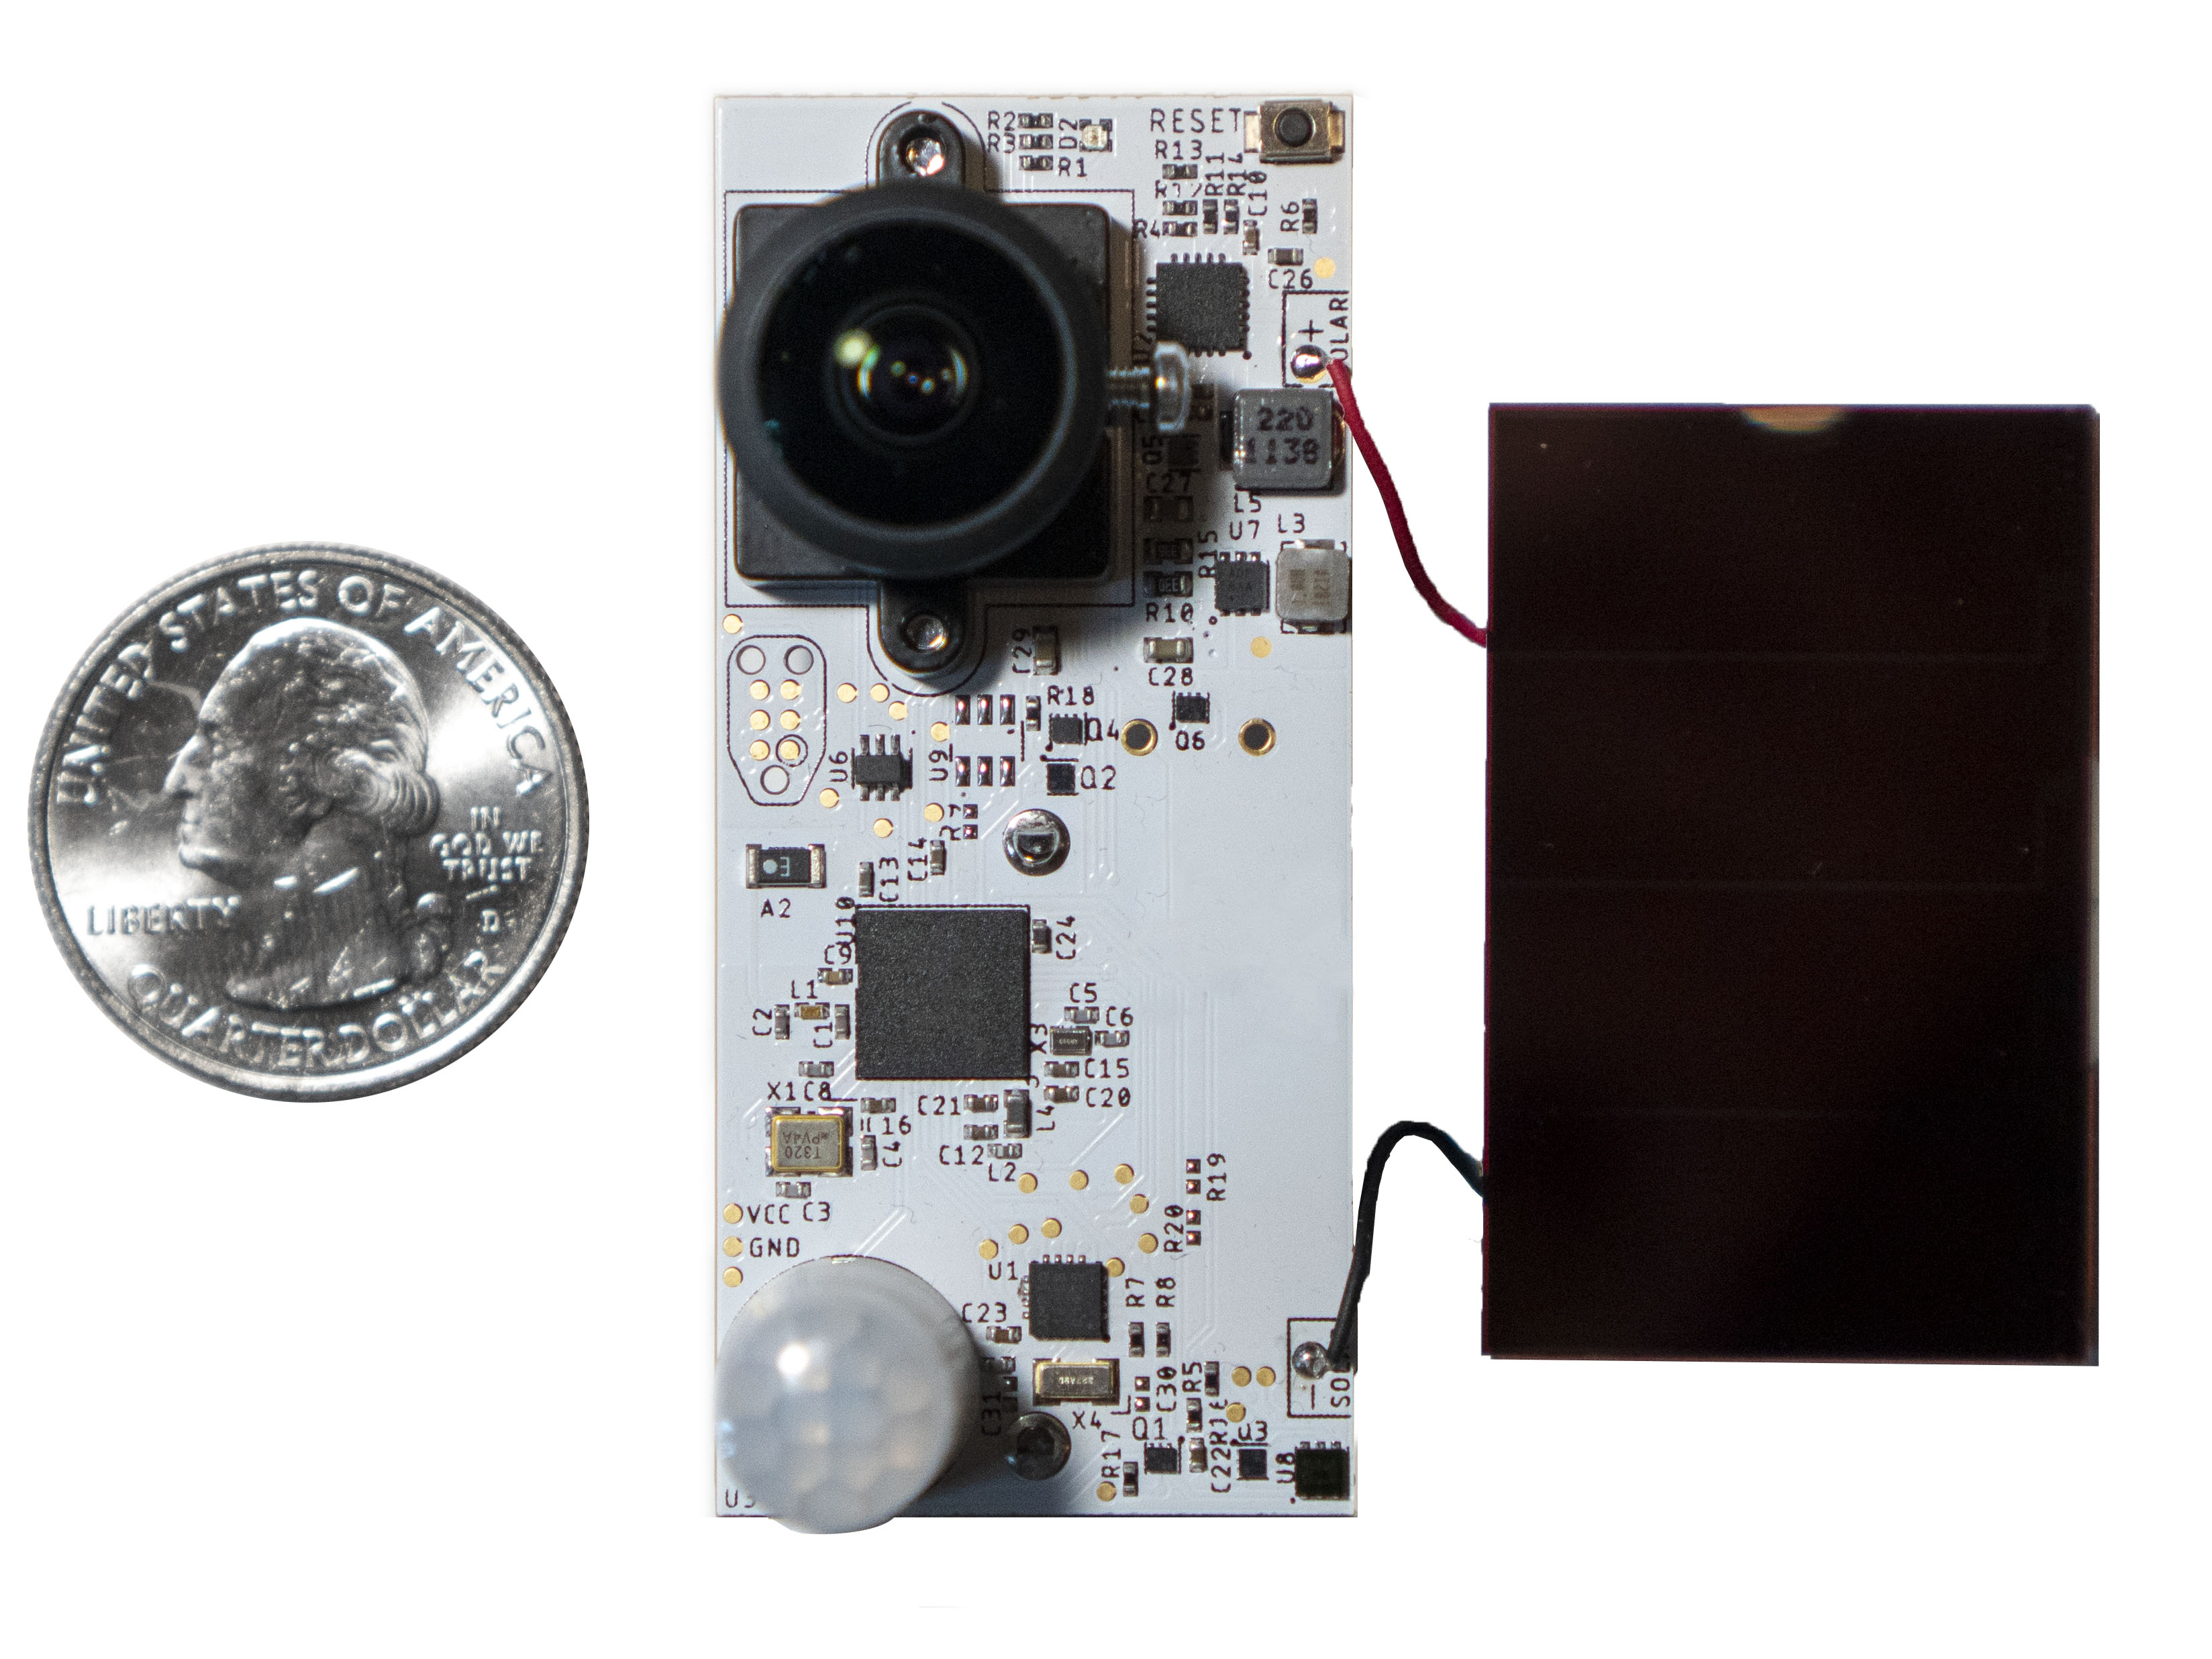
\includegraphics[width=\columnwidth]{images/platform_quarter.jpg}
\vspace{-2\baselineskip}
\caption{ \name{}. 
    \normalfont{A wireless camera platform for indoor computer vision applications. To achieve a multi-year lifetime, we employ energy harvesting with a photo-voltaic panel. A quarter is included for scale. \name is capable of local inference as well as full image transmission to cloud image processing pipelines. The platform is 10\,mm thick, and has a rechargeable and non-rechargeable battery on its backside}
}
\end{definefigure}
\placefigure{fig:platform}

\section{Introduction}
Image inference, including classification and object detection, has been one of the most active areas of computer science and machine learning research. However, due to the cost and difficulty of deploying wired cameras, applications based on continuous image sensing is untenable. This is especially true for indoor applications, where camera density must be higher for sufficient coverage.

Indoor wireless camera sensors have been heavily researched and commercialized over the past fifteen years, but due to the technology available at the time, as well as incompatibilities between design decisions and longevity, these platforms are typically limited to lifetimes of at most weeks to months~\cite{rowe2007firefly,rahimi2005cyclops,blinkindoor,wyzeoutdoor,josephson2019wireless}. 
Deployment of these platforms beyond small or temporary installations remain a challenge due to the cost of frequent battery replacement.
With the confluence of new and improved COTS technology, like low power processors, radios, and image sensors, it is worth revisiting the design of wireless camera sensors. 

Recent improvements in microcontrollers go beyond lower power \cite{kim2018system}. Processors now include hardware floating point support, single cycle multiplies, and data-parallel instruction (SIMD) support. The promise of new dedicated accelerators provides the potential of significant improvements in inference performance on low power systems~\cite{armm55,himaxwiseeye}. This has led to renewed interest in performing complex local inference on a battery budget, especially as transmitting large data like images is traditionally very expensive. However, radios have also become far more power efficient, which again muddies the conventional wisdom. Indeed, it is now much cheaper to transmit large data to a more capable system. Desktop or server class machines handily outclass their low power microcontroller and accelerator brethren on performance, providing the ability to perform more complex and accurate inference, if only data can be efficiently delivered to them.
%Regardless of recent improvements, microcontroller and accelerator performance will continue to pale in comparison to desktop and server class computing systems. 
This is especially true as memory has not scaled at the same pace as processing.
This rapidly changing design space points to a requirement for a flexible architecture and framework for thinking about what applications are most suited for local processing versus cloud offload.
% or data transmission.

In this work, we present \name, the first wireless, energy-harvesting camera platform capable of capturing and transmitting an image every ten minutes for half a decade in indoor environments.
\name represents a culmination of recent work on low power camera sensors~\cite{josephson2019wireless,nardello2019camaroptera,naderiparizi2015wispcam} and energy harvesting sensor platforms~\cite{jackson2019capacity}. \name features a hierarchical energy harvesting system that couples a small rechargeable battery with a backup non-rechargeable battery. This combination provides the system with a long and reliable lifetime. The longevity and reliability of the platform make it suitable for long-term, low-maintenance deployments. Images captured by \name are capable of driving applications based on object detection, like people counting or interaction tracking. With default, pretrained weights, an object detection model is able to detect a person in \name images from 20 meters away.

\name is capable of performing both local inference and transmitting full images end-to-end to more powerful systems. Local inference potentially requires less energy than image transmission, and also provides significantly better privacy guarantees. In cases where privacy is not as much of a concern, image transmission to a more capable endpoint increases the flexibility and performance of inference run on images. Privacy can still be guaranteed if images are transmitted only within a local network.
We examine the implications of both architectural choices with respect to capability, energy, and latency.

Our results show that on modern SoCs, transmitting images surprisingly enables longer lifetimes and improved inference. While this conclusion is unique to indoor wireless camera sensors 
whose footprints are not dominated by their energy harvester or storage, its general methodology can be applied to other application spaces as well.
%
Through this conclusion, we develop an end-to-end architecture that makes images captured by \name accessible to data collectors and application builders. \name provides a scalable and easily deployable method to quickly gather visual data for machine learning training or datasets. Images collected by \name are easily integrated into popular computer vision and machine learning frameworks like OpenCV, TensorFlow, and PyTorch. Using these tools, high level applications can be built to drive visual applications like building occupancy counting for more efficient energy management and critical infrastructure monitoring atop a long-lived deployment of wireless \name devices.

%Additionally, privacy is a serious concern, and we demonstrate that \name is capable of some local inference. In cases where applications require capability over privacy, images can be transmitted end-to-end to the cloud, or to a more local endpoint. 
%This provides the option to still maintain some privacy when transmitting images.




\chapter{Background}
\label{chap:background}
System researchers have been developing wireless sensors for over twenty years.
Sensor systems research is uniquely application focused, with many seminal works involving real applications and deployments~\cite{juang2002energy,mainwaring2002wireless,tolle2005macroscope}.
A lot of other research has been focused on developing and utilizing new and improved technology for wireless sensor designs.
%to enable new sensor modalities, regimes, and applications.
Over the past two decades, microcontrollers have vastly improved in processing speed and capability, sensors have continued to shrink in size, and wireless communications have increased throughput and range.
Across the board, all wireless sensor components have also substantially increased their energy efficiency.
However, the availability of power and energy remain limiting factors for wireless sensor designs.

The energy density of non-rechargeable batteries has not improved at the same rate as as other wireless sensor components.
While newer, more efficient sensors are able to do more with the limited energy available to them, battery-based sensors are still limited in lifetime and have the potential to produce substantial battery waste.
For longer deployments, or in applications where the size and weight of a non-rechargeable battery was untenable, researchers have also developed energy harvesting solutions for wireless sensors.
Energy harvesting sensors do not have concretely limited lifetimes, but they are inherently limited by the availability and consistency of harvestable power.
Like battery technology, the efficiency of energy harvesting methods have not increased at the same rate as other sensor technology, and specialized energy harvesting power management ICs are already highly optimized to extract energy from many sources~\cite{adp5091,bq25505,matrix_prometheus}, with few exceptions~\cite{josephson2020farming,marcano2022soil}.
System designers are left with two unsatisfying options.
Depending on an application's lifetime, maintenance, and quality of service requirements, batteries may offer insufficient longevity, and energy harvesting may allow insufficient availability.
This chapter seeks to explore the myriad of traditional and contemporary methods of powering sensors and their trade-offs
with the goal of identifying common application requirements and how various power supply designs satisfy those requirements.

%The field of wireless sensor system design
%20 years of sensor research
%A lot of this work is driven by new and improving technology
%Technology improvements enable new applications
%It is difficult to navigate the technology landscape to determine proper design for a given application
%Designers are left making design choices based on technology instead of what an application requires
%This section seeks to examine past work and the modern technology landscape, and contextualize these within past and present application requirements.

\section{Methods to Power Wireless Sensors}
\label{sec:background:methods}
All wireless sensors require electrical energy to function.
Most simply and most commonly, energy can be provisioned in a finite energy storage such as a battery, also known as a primary cell.
In situations where there is harvestable energy, it can be captured and stored in rechargeable storage, or a secondary cell.
The next sections describe prior work in both research and industry regarding preallocation and energy harvesting wireless sensor design.

\subsection{Energy Preallocation}
Primary-cell
batteries are the preferred
method of powering sensors for both academic experimentation
and commercial and industrial applications.
The Telos family of motes, originally designed in 2004~\cite{polastre2005telos},
are still the wireless platform of choice for some modern research projects~\cite{mohammad2018codecast,li2019privacy}.
The Hamilton mote is a more modern example that seeks to provide a cost-effective and longer-lived alternative to older motes~\cite{andersen2017hamilton}.
Besides research platforms, the majority of commercial smart home sensors, like those offered by Ecobee, Honeywell, Lutron, Nest, Phillips, among many others, all opt to use non-rechargeable batteries as their source of energy
~\cite{ecobeeSensor, honeywellThermostat, lutronSolutions, googleNestTemperature, hueSensor}.
Industrial offerings from Emerson, GE, Honeywell, and others mostly utilize non-rechargeable power cells in their wireless sensors~\cite{emersonRosemount,GEInsightMesh,honeywellOneWireless}.
The use of primary-cells is popular in commercial and industrial sensing because they enable sensors with predictable lifetimes that are easy to
design, simple to program, and reliable to operate.
However, a finite energy storage provides a finite lifetime, meaning battery replacement is inevitable.
To achieve a long lifetime, sensor designers must often sacrifice constraints on size to accommodate a larger battery.
However, advances in energy efficiency and battery longevity have resulted in reasonably sized commercial and industrial sensors that can last up to 10 years without battery maintenance~\cite{emersonRosemount,honeywellOneWireless, lutronSolutions}.

\subsection{Energy Harvesting}
%Prior work regarding energy-harvesting sensor systems can be broadly
%divided into two categories: those which make use of intermittent computing
%techniques and those which do not.
%Intermittent systems often exist in a regime of unreliable and ultra low harvester power, where
%operation and uptime are not guaranteed. As such, they often lose power and
%reboot while intermittently working through a sensing task.
%A wealth of work has been devoted to
%making these systems usable and reliable.
%Other energy-harvesting systems, especially those deployed outside, have access
%to significantly more harvestable energy and are able to store more of this energy
%for later use, so they
%do not use intermittent computing techniques to complete their workloads.
Instead of preallocating energy, a system can utilize external sources of energy.
A system that harvests energy is not as limited in lifetime as a primary-only system, and depending on the durability and longevity of its harvester and energy storage, can persist indefinitely.
However, the quantity and consistency of external energy can vary widely.
If the energy is predictable or reliable, an energy harvesting system can operate reliably.
If the source is unpredictable and insufficient to power a system continuously, the system may operate inconsistently if it does not have sufficient energy storage to buffer in times of insufficient income.
Capacitors, supercapacitors or batteries are all options to buffer energy when external energy is variable.
%At one extreme of power delivery, a wireless sensor can be powered by a reliable source, like wired power.
%As much as it seems like an antithesis to "wireless" sensors, wired power is a solution for a class of applications where using a battery is more costly than installing wired power.
%This is especially true for applications that are monitoring powered devices or measuring mains power.
%For example, the Powerblade power meter is connected to AC mains power for both measurement and power supply~\cite{debruin15powerblade}.
%Its proximity to readily available AC power and its small form factor make the inclusion of a battery infeasible compared to scavenging off mains power.

The majority of energy harvesting wireless sensors depend on unreliable external sources of energy.
They utilize photovoltaic, thermoelectric, piezoelectric, ambient RF harvesting, or other methods to scavenge energy from their environment.
Parameters like harvester size or surface area, impact the amplitude of power delivered to the sensor,
while the size and capacity of the rechargeable storage determines how much energy can be buffered.
%This device class can be further differentiated by how captured energy is stored. Intermittent, or batteryless systems, eschew both non-rechargeable and rechargeable batteries and utilize capacitors and supercapacitors for energy buffering. The choice of a (super)capacitor buffer significantly limits the amount of energy capacity available to the system, reducing its capability to cache energy in times of drought. This choice is predicated on the assumption that rechargeable batteries are less suitable for energy harvesting applications. However, most energy harvesting systems, particularly those that utilize outdoor photovoltaic harvesting, utilize rechargeable batteries.
Energy harvesting sensors
have largely been developed for use in environments with plentiful harvestable energy.
%and have been designed with sufficient capacity to capture this energy
Most examples of energy harvesting research devices are deployed outdoors with photovoltaic cells~\cite{jiang2005perpetual, kansal2007power, corke2007long, lin2005heliomote, taneja2008design, adkins2018signpost}.
This is also true of many commercial and industrial sensor systems like weather and air quality monitoring stations~\cite{davis_weather}, trail cameras~\cite{spypoint_camera}, and traffic cameras~\cite{wanco_traffic}.
Industrial products have also leveraged temperature gradients and vibration to power sensors. The Perpetua Power Puck and Tile are thermoelectric generators designed for high temperature monitoring of critical infrastructure like steam pipes, hot tanks, and other equipment in high temperature environments~\cite{perpetua}.
Perpetua harvesters are compatible with the same Emerson, GE, and Honeywell sensor systems as a drop in replacement for the default non-rechargeable power supplies. Other companies, like ReVibe and Kinergizer, are utilizing piezoelectric harvesting for industrial vibrational monitoring~\cite{revibe,kinergizer}.

There have been fewer research, commercial, and industrial sensors developed for indoor environments, or other environments that lack light, a large temperature gradient, or perpetual motion and vibration.
This is because it is more difficult to design a lower power system to match a lower power income, even with newer and more efficient technology.
Despite these difficulties, researchers and industry have developed sensors for applications with limited access to harvestable energy.
Researchers have followed two distinctly different approaches for indoor energy harvesting.

Some of the first attempts at bringing energy harvesting indoors consisted of power supply architectures similar to those of their outdoor counterparts, in that they utilized rechargeable batteries for energy storage.
The EnHANTs sensor used an indoor photovoltaic panel to charge an intentionally oversized nickel-metal hydride (NiMH)
battery, with plans to eventually use a thin-film battery~\cite{gorlatova2009challenge,margolies2015energy}.
DoubleDip utilized thermoelectric harvesting to charge a lithium-manganese battery~\cite{martin2012doubledip}.
The batteries used by EnHANTs and DoubleDip are examples of older technology that had numerous limitations.
Early rechargeable batteries offered short cycle lifetimes and low charge and discharge current capabilities.
The cycle lifetime limit results in systems with limited longevity, even though they utilize energy harvesting.

Simultaneously, researchers at University of Washington and Intel Research Seattle began experimenting with computational RFIDs (CRFIDs) to create battery-free sensors~\cite{sample2008design}.
These researchers noted the limited storage of non-rechargeable batteries, and the limited cycle lifetime of rechargeable batteries.
Instead of batteries, these systems utilize small capacitor-based energy buffers that are able to store just enough energy to complete a small atomic task, be it operating a sensor, transmitting a packet via RFID backscatter, or performing some amount of computation.
While the longevity of CRFIDs are not limited to to the lifetime of a battery, they require the proximity of an RFID reader to provide power and bidirectional communication.
Since the development of CRFIDs, and as technology has continued to improve in efficiency, researchers have extended the technique beyond RFID to systems with active radios and other harvesting methods, including photovoltaic, piezoelectric, and thermoelectric harvesting~\cite{yervaGrafting12, debruin2013monjolo, hesterFlicker17, colinReconfigurable18, nardello2019camaroptera}.
%This approach has since become very popular, and the utilization of batteries for modern indoor wireless sensors is uncommon.
The majority of modern wireless sensor platforms build by researchers are batteryless, with many convinced that batteryless designs are the future for wireless sensor power supply design~\cite{hesterFlicker17,colinReconfigurable18,fraternali2018pible,truong2018capband,shukla2019skinnypower,hester2017future}.
Despite the excitement around batteryless designs, they exhibit some serious detracting qualities that may limit feasibility and adoption for many applications.
The next section explores the design and development of batteryless systems in more detail and describes the benefits and trade-offs of the design.
%However, the greater energy capacity provided by batteries allows these designs to avoid the complications of frequent power interruptions.

%Some
%devices have also embraced backup primary-cells to further ensure
%reliable operation.
%In the middle, in environments with sufficient and predictable available energy, designs can scavenge energy and store it in a rechargeable battery to power their workload.
%Energy harvesting in industrial environments is also possible with sufficient heat differential or vibrational sources~\cite{perpetua, kinergizer}.
%However, the adoption and application of such harvesting methods is limited and non-rechargeable batteries remain the most popular option for powering industrial sensors.
%Notably, Prometheus utilizes a supercapacitor as a short term energy store, and when full,
%charges a backup rechargeable lithium battery~\cite{jiang2005perpetual}. At
%the time of its design, lithium cells offered highly limited recharge cycles,
%and by utilizing a supercapacitor, much of this
%charge-discharge volatility was masked from the secondary-cell, extending its lifetime.



%DoubleDip notes that supercapacitors offer
%lower energy density and higher leakage when compared to batteries, but admits
%that the lithium-manganese chemistry suffers from low maximum output currents
%and a limited number of charge-discharge cycles.
%While the limitations of past batteries have slowed their adoption in
%low energy-harvesting scenarios, we claim that recent developments in battery
%technology will enable higher capacity energy storage without these trade-offs.


%\subsection{Energy Capture and Preallocation}
%
%Regardless of which energy store is used, energy-harvesting systems will
%experience some degree of uncertainty regarding energy income.
%A non-rechargeable
%backup energy store can be utilized to mask this uncertainty, cold
%start electrical components, and provide consistent, reliable, and lively operation.
%A third design archetype is a combination of the first two:
%external energy capture paired with a backup non-rechargeable cell.
%While this archetype makes sense from the perspective of maximizing system lifetime and reliability, it is not commonly employed.
%The Pressac line of supercapacitor-based energy-harvesting sensors
%use a battery backup to obtain an estimated 10 years of continuous, reliable operation~\cite{pressac}.
%%This work suggests that these sensors could significantly
%%increase their lifetime by using a larger secondary energy store.
%There has been little
%exploration on the benefits of this hybrid design and the use of
%primary-cells to avoid intermittency,
%and provide baseline reliability. This dissertation seeks to explore this design point in more detail.





\section{Batteryless Energy Harvesting}
\label{sec:background:batteryless}
The batteryless, or intermittent, sensor movement has abandoned batteries (both rechargeable and non-rechargeable) under the assumption that current battery technology has too many detracting qualities to be suitable for energy-harvesting wireless sensors.
Most notably, they argue that rechargeable batteries provide insufficient lifetimes to build long-lasting deployments~\cite{hesterTragedy15, hesterFlicker17, hesterTimely17, hester2017future, colinReconfigurable18, luciaIntermittent17, yervaGrafting12, majid2020continuous}.
Batteryless systems instead utilize capacitors, some types of which offer functionally infinite lifetimes~\cite{kemetLife}.
However, capacitors and supercapacitors provide much less energy storage compared to batteries.
%. Ceramic and tantalum capacitors possess functionally infinite lifetimes, while supercapacitors offer lifetimes on the order of decades to a century~\cite{kemetLife}.
%The relatively small energy storage afforded by capacitors and supercapacitors is a fundamental limitation and is the trade-off when prioritizing power supply lifetime over any other performance metric.
Due to this, a batteryless design results in two major drawbacks:
at any given time, a batteryless system is limited to the energy provided by the short discharge cycle of its capacitor bank,
and the availability of the system is determined by the consistency and intensity of energy income.

A batteryless system can technically perform the operations of a wireless sensor but it may not perform them well.
When these systems are harvesting enough power to turn on and operate, they can only perform operations that require less energy than their capacitor storage can hold.
Often a batteryless system's income power is intermittent, resulting in a system that operates intermittently.
When harvestable energy is unavailable, batteryless systems quickly deplete their
small energy stores, and lacking any future income,
they power off and lose
volatile state, potentially in the middle of an important operation and for an extended and unknown period of time.
The intermittent reality of many harvesting sources necessitates careful management of energy
%and complex software control of volatile state
and detailed and thorough software optimization
to ensure that \textit{any} operations can be completed.

Despite these complications, the concept of an immortal wireless sensor is tantalizing, and is the driving motivation behind batteryless systems research.
%This potential for extremely long-lived sensors has led to significant work to enable and improve batteryless systems.
This has resulted in a wealth of batteryless systems research, the majority of which is focused on developing software solutions that manage and preserve volatile state across power failures.
State preservation has the potential to extend the runtime of sensor workloads beyond that of a single capacitor buffer discharge cycle, and is useful for building more general and capable systems.
Batteryless devices are also difficult to debug and develop software for, as in addition to software bugs, energy is no longer guaranteed at any point during execution.
To this end, researchers have also built tools to recreate energy conditions to help diagnose and fix intermittent energy bugs.
%Platform builders have also experimented with novel hardware techniques to increase responsiveness by reducing charging hysteresis.
In addition to software solutions, researchers have designed hardware platforms that maximize individual component availability, as well as platforms that dynamically tune capacitance to meet individual operation energy requirements.
%The software solutions presented by batteryless researchers are solutions developed for self-imposed problems stemming from limited energy storage, and hardware solutions offer marginal improvements to system responsiveness at a prohibitive cost.
The next sections discuss various system designs, tools, and software and hardware techniques developed to alleviate the drawbacks to batteryless systems.
%Energy-harvesting systems that rely
%on small (super)capacitor energy buffers are commonly referred to as intermittent systems, as they only store enough energy to perform single atomic tasks, and are unable to operate when external energy is not present.
%Many choose to employ
%capacitors as an energy buffer due to their theoretically infinite lifetime,
%but are limited to small energy capacities, and are only as reliable and
%lively as their source of harvested energy.
%In situations of energy drought,
%these platforms quickly deplete their
%small energy stores, and lacking energy,
%they power off and lose
%state, potentially in the middle of an important operation or for an extended period of time.
%Due to this reality, researchers have spent the past decade
%designing more predictable and usable batteryless systems. This has resulted in several different hardware and software design methods and techniques for intermittent systems.

\subsection{Forward Progress and State Retention}
The type and amount of work that is possible within the energy envelope of a single discharge cycle of capacitor or supercapacitor buffer is severely limited.
%Applications and devices that employ a one-shot technique are
Batteryless systems are generally only able to perform a few seconds or less of computation, or send a single packet before depleting their capacitor storage and powering off, even with modestly sized supercapacitors~\cite{yervaGrafting12,hesterFlicker17,colinReconfigurable18,nardello2019camaroptera}.
This section discusses the techniques developed by batteryless researchers to perform interesting sensing under unpredictable power loss.

\subsubsection{One-shot Intermittency}
\label{cha:background:one-shot}
One of the simplest methods employed by batteryless systems does not bother to attempt to retain state across power failures and reboots.
One-shot intermittent designs instead just allocate enough capacitance to turn on and perform a simple predefined task, like sending a packet.
This method is reminiscent of the simple reply behavior of RFID tags, upon which the design of early intermittent systems is based on~\cite{sample2008design}.
These systems may act as a simple beacon~\cite{campbell2016cinamin,saoda2019no}, or a sensor~\cite{yervaGrafting12, debruin2013monjolo, campbellEnergy14, campbellThermes14}.
For some platforms, most notably the Monjolo family of devices, the rate of harvesting is used as the sensor itself. Every wake-up and transmit event corresponds to an amount of energy harvested, and can be used to quantify the harvested phenomenon~\cite{campbellThermes14, campbellEnergy14, debruin2013monjolo}.
This method of coupling harvesting and sensing is the only way to ensure that interesting sensor data is observed by a batteryless sensor.
Otherwise, when a batteryless sensor is built to sense a phenomena independent of the harvesting method, it is inevitable that changes in the sensed phenomena will be missed because the sensor is offline.
Even when sensing and harvesting is coupled, a one-shot batteryless design often does not have the energy required to support message retransmission in the case of packet loss, or generally support any network reliability mechanisms.
Any observation may be lost upon packet reception failure, and the next time the sensor wakes up it will only have enough energy to be concerned with transmitting its most recent observation.
This one-shot method is relatively simple compared to other approaches to batteryless software, but it still requires tedious cold-start software optimization and capacitance tuning to allow the device to power on and complete its workload within the constraints of its tiny energy storage.
This severely limits the generality of systems developed with this approach.
Performing any sensing or computing outside of the hardware's intended use case is often not possible.
Like all batteryless sensors, it is also impossible to distinguish between sensor failure and a lack of energy.

\clearpage

\subsubsection{Checkpointing}
Given the limitations of the one-shot technique, researchers have developed tools and techniques for
ensuring forward progress across system reboots to enable longer and more complex workloads than a single capacitor bank can support.
%Since the development of the WISP platform~\cite{sample2008design}, researchers have continuously developed software tools, methods, and techniques to save state and resume operation across power outages, allowing for longer running computation or transmitting more data than a single capacitor bank would support.
One method of enabling forward progress is checkpointing,
where important volatile state is saved at predetermined and run time locations in code prior to a power outage, and restored upon rebooting. Many methods have been proposed, using both static and dynamic methods.
Mementos utilizes a modified LLVM compiler, as well as a run-time library, to automatically place checkpointing triggers within a program~\cite{ransford2012mementos}. During run-time, at these trigger points, Mementos measures the system voltage, and if low enough, portions of volatile state are written into non-volatile flash before turning off.
The introduction of new non-volatile technologies like Ferroelectric RAM (FRAM) allows more energy- and time-efficient checkpointing, while simultaneously simplifying the state retention logic.
Hibernus does not use predefined trigger points, and instead utilizes a hardware interrupt to detect a low system voltage threshold, and immediately copies volatile state to FRAM~\cite{balsamo2014hibernus}. This state is subsequently restored on a rising voltage interrupt.
Checkpointing is an effective method for enabling forward progress. However, software development with checkpointing can be very difficult to develop and debug, and writing and restoring state can become prohibitively expensive in time and energy as the amount of volatile state increases.
%improving the programmming and debugging experience for batteryless programmers.
%Writing programs for intermittent operation introduces bugs that do not exist with continuous operation, and requires more advanced debugging techniques to address them.

\subsubsection{Batteryless Debugging}
For batteryless systems, it
is very difficult to properly and correctly develop software, especially when non-volatile memory like FRAM is involved.
One-shot system software is difficult to tune and optimize to complete all within the energy provided by capacitor storage.
For checkpointing systems, if checkpoints are improperly placed such that atomic blocks are not completed entirely before power loss, and yet their partial state is recorded in non-volatile memory,
it can result in inconsistencies between volatile and non-volatile state.
Software development and debugging for batteryless systems must also consider energy state.
To this end, researchers have developed hardware-software debugging tools that emulate and replay energy state based on energy trace captures.
Ekho is an energy emulator that recreates and repeats energy harvesting conditions for low power energy harvesting devices~\cite{hester2014ekho}.
Another tool, the energy-interference-free debugger (EDB), also replays energy state, specifically for intermittent systems~\cite{colin2016energy}.
EDB augments normal interactive debugging tools like GDB to allow real time playback of energy state, in addition to interactive program debugging.
While these tools are useful and necessary for ensuring correctness in batteryless development, they do introduce substantial complexity on top of an already complex embedded software debugging and development toolchain.

\subsubsection{Safe Forward Progress}
While conceptually simple, checkpointing is not a perfect solution to saving state, especially as that state begins to increase in footprint with increasing application complexity.
There is an upper bound to the size of checkpoints, where the energy required to save and read state to and from non-volatile memory exceeds that offered by various capacitor storage sizes.
The advent of FRAM (as well as other non-volatile RAM technologies) results in methods that can avoid explicitly saving and reading back the majority of application state. State that would normally reside in volatile RAM can now be placed within non-volatile memory, allowing this state to persist across power outages.
While this seems like a straightforward solution to preserving state, it is complicated by the shrinking
boundary between volatile and non-volatile state. Often both SRAM and FRAM are memory mapped and accessed the same way. Writes and reads to either are indistinguishable to the programmer and compiler.
Code is often executed multiple times through the course of intermittent execution, and if volatile and non-volatile state are not carefully managed and accessed by the program, re-execution of various code sections can result in consistency violations~\cite{maeng2017alpaca}.
The aforementioned debugging tools can help to detect and fix intermittency bugs during runtime testing. However, many researchers have developed solutions to avoid these bugs by design.
Task-based programming frameworks and models like
Chain~\cite{colin2016chain} and Alpaca~\cite{maeng2017alpaca}
ensure forward progress and prevent intermittent consistency bugs.
The task model of execution splits a software application into idempotent code blocks that read inputs from other tasks, and upon completion write their own results to channels of non-volatile memory. This has the effect of increasing task throughput in addition to ensuring safe forward progress.

\subsubsection{The Wrong Abstraction}
While effective in ensuring safe forward progress, all of these techniques introduce
significant software and compiler complexity.
%on top of an already complex embedded software development toolchain.
They also necessarily limit programming scope to defined frameworks and concepts to ensure various constraints and guarantees of safety.
Batteryless programmers must learn and adopt new programming models that incorporate potentially unfamiliar concepts like tasks, channels, and flows~\cite{colin2016chain,maeng2017alpaca,hesterTimely17}.
Once programmers have mastered the new patterns and methods of batteryless programming, intermittency is largely hidden from them.
This is by design and one of the main goals of these programming models and frameworks.
However, the abstraction of continuous progress is more harmful for application developers than helpful.
%To a programmer, the abstraction of continuous progress is easily conflated with continuous operation.
This abstraction provides the illusion of continuous computing progress in processor time, while robbing programmers and users of any meaningful notion of progress in wall clock time.
Continuous operation of a batteryless systems is often impossible, and software methods for forward progress only guarantee \textit{eventual} task completion.
While these techniques may make it easier to program batteryless systems,
the abstraction of continuous forward progress is misleading regarding the timeliness and availability
of systems that employ them.
These techniques do not address the needs of any application that requires availability or timeliness of data.
System designers and programmers are left without a way to reason about and quantify the actual performance of applications built on top of these abstractions that mask inherent system unreliability.
%An abstraction that guarantees forward progress without feedback or some metric of \textit{what} that forward progress consists of or how long it takes removes agency from the programmer.
%This abstraction makes it extremely difficult to reason about the actual reliability and availability of applications built on top of fundamentally unreliable systems.
%The eventual forward progress allowed by these techniques inflates the perceived utility of these systems,
%as they suggest continuous and eventual operation and progress. In reality, they operate with no guarantee of reliability or even eventual task completion.
%This results in systems that technically function in the sense that they occasionally perform a task when energy is available, but there is no guarantee as to how long a task will take to complete, nor that they are capturing an accurate representation of a sensed phenomenon.
%their overall performance and reliability is unpredictable and varies widely depending on their environment and deployment location.
%No amount of software techniques and improvements will address the unreliability of batteryless systems, as it is a fundamental result of a design with insufficient energy storage to support continuous and reliable operation.

\subsection{Timeliness and Availability}
While convenient during programming, the abstraction of continuous operation without a notion of real performance does not result in responsive and available batteryless systems.
The task-based models ensure safety and improve performance over checkpointing-based approaches, but they
do not consider or provide solutions for increasing batteryless system responsiveness and availability,
two qualities that are especially important for wireless sensing.
Timeliness and availability are goals that are generally at odds with the reality of batteryless sensing, as no guarantees can be made about energy income and thus the timeliness of event completion or system availability.
A batteryless system's intermittent execution can span unknown periods of time, where it iteratively works on a task whose results may be stale and no longer useful by the time it finishes. There is also no way to ensure that a batteryless system is awake to witness a given event.
Despite this, researchers have developed both software and hardware solutions in attempts to improve batteryless responsiveness and availability.

\subsubsection{Software Timeliness and Availability}
Mayfly~\cite{hesterTimely17} and InK~\cite{yildirim2018ink} are task-based software frameworks like Chain and Alpaca. In addition to ensuring safe forward progress, they also attempt to maximize system timeliness and availability respectively. Mayfly associates tasks and the data they produce with deadlines, and maintains time through power failures.
After a datum's deadline passes, it is discarded and energy is not used to further process or transmit it.
This approach prioritizes fresh data, and allocates more energy towards completing tasks that can be completed within their deadline.
This enables applications that depend on timely data, such as activity recognition. Alpaca and Chain are unsuitable for such applications, as they are unable to distinguish between expired irrelevant data and new fresh data.
While it increases the timeliness of a system, Mayfly does not increase the amount of reported data by a system or its availability, as it cannot increase the energy available to the system. By design, it must sacrifice stale, potentially important data in order to report fresh data.
It is uniquely suited for applications that are only concerned with close to real time data.

InK prioritizes availability by incorporating timers, interrupts, and event handling into a batteryless context.
The runtime utilizes sleep states and low power interrupts to persist for longer periods and increase the likelihood of detecting and capturing events. It also utilizes an ultra-low power timer subsystem to ensure timekeeping across power failures.
With these improvements, a system using Ink is able to capture 14x the number of events over the same system using Alpaca.
While this seems like a dramatic increase, Alpaca was not designed with event detection workloads in mind. It performs abysmally
when applied to such tasks. With controlled solar harvesting conditions, a system running on Alpaca was only able to capture less than 5\% of events.
Comparatively, the system with Ink was only able to capture slightly over half of the events even when in the same light conditions~\cite{yildirim2018ink}. The authors did not compare the performance of these runtimes with that of a traditionally programmed and continuously powered embedded system, so there is no baseline comparison.

While these approaches increase the timeliness and availability of a system,
it is \textit{impossible} for a batteryless system without continuous energy income to ever approach 100\% event detection or data capture and transmission reliability.
There will be always be periods of time where there is no available energy, a batteryless system will remain off, and important events will remain undetected and important data will be discarded as it grows stale.

%Beyond software techniques to improve the intermittent programming experience, ensure forward progress, and increase reactivity,
%researchers have also developed novel hardware and system designs to
%increase the responsiveness and availability of batteryless systems.
%Many hardware techniques focus on the fine-grained management
%of capacitor charging hysteresis.
%Unlike the relatively stable voltage provided by a battery, a capacitor's voltage is related to the square root of stored energy. This means that during a discharge cycle, an intermittent system will experience a pronounced voltage drop from a maximum $V_{max}$ to a minimum $V_{min}$.

\subsubsection{Hardware Hysteresis Management}
\label{sec:background:hhm}
Beyond software techniques, researchers have also explored building specialized hardware solutions to increase system availability.
Batteryless system operation is generally tied to a full swing capacitor charge/discharge hysteresis. Once enough energy is captured, a batteryless system will begin executing its workload until it has exhausted its stored energy.
The general rule of thumb for batteryless system capacitor sizing is that it must hold enough energy to support the most energy intensive atomic task of the system, such as operating a sensor, performing some quanta of computation, or transmitting a single radio packet~\cite{nardello2019camaroptera,colinReconfigurable18, shukla2019skinnypower, hesterFlicker17}.
This represents the smallest amount of energy storage that results in a feasible system with checkpointing or other forward progress mechanism.
All batteryless systems operate within the bounds of capacitor storage voltage thresholds.
The energy stored within a capacitor is directly related to the voltage across its electrodes.
\begin{equation}
\label{eq:cap_energy}
    E = \frac{1}{2}C(V_{max}^2 - V_{min}^2)
\end{equation}
The upper hysteresis threshold $V_{max}$, the point at which the device is charged and turns on, is the voltage at which a capacitor is full, and the lower threshold $V_{min}$, the point at which the system turns off, is the minimum
operating voltage of the components in the system.
Smaller capacitors can charge to an upper
threshold and turn on faster, but store less energy.  Larger capacitors store more energy, but charge slower.
Hysteresis management
techniques attempt to combine different sized capacitors to
optimize the charging time and available energy for specific tasks.
Managing hysteresis also allows for more platform generality, as the capacitor storage can be optimized for various operations and workloads.
Notable examples of platforms that utilize this technique are the Flicker and Capybara systems~\cite{hesterFlicker17, colinReconfigurable18}.

The Flicker
platform practices federated energy storage, where each module (sensor, radio, microcontroller) has its own built in capacitor that is tuned to the task it is expected to perform~\cite{hesterFlicker17, hesterTragedy15}.
This has the
effect of allowing various components to charge their storage quickly and begin operating before other parts of the system turn on or are needed. This also
isolates power failure to independent components.
Federated storage provides marginal improvements with regard to component availability and energy harvesting efficiency. A federated approach provides an average increase of 6.7\% for microcontroller uptime (from 64.2\% to 70.9\%) and a 1.5\% increase for radio uptime (from 3.8\% to 5.24\%) over a single duty cycle. Likewise, a federated approach provides at most a 10\% improvement in energy harvested over a duty cycle~\cite{hesterTragedy15}.
A federated approach incurs overhead involving additional hardware complexity in the form of voltage monitoring circuitry as well as more complex software to manage and make use of the additional voltage information. The additional hardware increases the size, cost, and energy overhead of the system.

The Capybara platform also manages capacitor hysteresis to increase system responsiveness and reactivity. However instead of using federated capacitor storage, it utilizes a central capacitor bank that can be dynamically resized~\cite{colinReconfigurable18}.
This is a more flexible approach than federated energy, where each hardware peripheral is designed with a specific amount of capacitance to support a predetermined task.
Capybara can resize its capacitor bank on the fly to match the energy required by an arbitrary task. This results in the lowest possible cold start and capacitor recharge times to support a given operation.
Under controlled conditions with consistent harvestable power, Capybara is able to detect 2-4x of events over a system with statically allocated capacitance. However, this improvement only detects 40-70\% of possible events, even under optimistic harvesting conditions.
To support this dynamic resizing, Capybara introduces an extremely complex and costly power system design that occupies significant board area.
The design includes five mixed capacitor and supercapacitor banks, four state-retaining switches for connecting the capacitor banks to the load and harvester, and a custom power distribution circuit to charge the configuration of capacitors.

These techniques are based on the assumption that a full swing capacitor hysteresis with full power downs are necessary and unavoidable. Batteryless systems are often not designed to support a low power sleep state with volatile state retention.
%This assumption is unique and common with batteryless systems, where uptime is severely limited by the system's active power and available energy storage.
%Energy must be micromanaged on the scale of milliseconds to seconds, which leaves very little slack to preallocate enough energy to enter and persist within a sleep state. Often, batteryless designs do not bother to optimize for a sleep state.
Sleeping is a difficult operation for systems with relatively little energy storage, as it is difficult to proactively retain enough energy to enter and sustain a sleeping state when future availability of energy is uncertain.
Additionally, energy must be micromanaged on a time scale of milliseconds to seconds.
The precision timing of entering sleep state at the correct capacitor voltage level is often not worth the engineering effort to implement when compared to allowing the system power off naturally. Thus, batteryless systems are not often optimized for sleeping.
For example, Capybara is by design an inefficient sleeper but has very low leakage when powered off.
Its power supply has a significant
``power overhead of the power system'' that limits the effectiveness of
any low power state besides being completely off~\cite{colinReconfigurable18}.
The decision to design around constant reboots incurs significant cost in energy and time. Without significant software optimization, the initialization of a processor, radio, and other peripherals is an expensive operation. If capacitor storage is allowed to leak (over the course of hours without any harvestable energy) the voltage may drop to a point that a boost converter must cold start.
Cold start is also very expensive, as harvesting ICs and boost converters are optimized for steady state operation and not cold start efficiency.
For example, the TI BQ25505 harvesting boost charger is capable of operating at \textgreater90\% efficiency at voltages higher than 1.5\ssi{\volt}~\cite{bq25505}.
However, its worst case cold start efficiency is 5\%, and requires at least 600\ssi{\milli\volt} input and 400\ssi{\milli\watt} instantaneous power to exit cold start.
Over the course of operation, a batteryless system will experience many repeated cold starts, resulting in wasted energy and time.

%While the design decisions to manage and fine-tune hysteresis make sense in the intermittent context, the importance placed on cold start optimization is specific to the power efficiency and limited energy capacity of a batteryless design.

%However, in times of gratuitous harvestable energy, a batteryless system should be able to maintain a low power sleep state for a long time, and avoid incurring the cost of repeated cold-start.
%Despite this, most batteryless systems assume the necessity of a full-swing operation, and their design abolishes the possibility of sleeping.

%Due to this, most intermittent system designs opt to fully discharge energy storage on every operation instead of sleeping. Because of this, batteryless system designers must often focus on optimizing the cold start of their system.
%In practice, if a system has the ability to enter a low power sleep mode with state retention, it can avoid frequent cold start and control its energy usage by willfully entering these
%states.
%With this operating principle, the benefits of hardware hysteresis management are limited to reducing cold start time and are workload independent.
%We show that the energy captured
%by these systems and their subsequent availability
%could be substantially improved by using larger energy buffers.

%Simultaneously sensing and harvesting the same phenomenon is one of the most effective use cases of batteryless sensors, however being able to simultaneously sense and harvest is not always possible, and is generally limited to light, temperature differentials, vibration, and RF sources.

\subsubsection{Redundancy for Statistical Availability}
Beyond software and hardware techniques for forward progress, timeliness, availability, and reactivity, researchers have also explored approaches that utilize cooperation within a network of batteryless devices.
Most notably, the Coalesced Intermittent Sensor (CIS) is an abstraction of a group of intermittent sensors that combines the availability of each sensor to increase the availability of the group as a whole~\cite{majid2020continuous}.
The CIS approach leverages the theoretical uniform distribution of the availability of an ensemble of sensors, each of which is intermittently operating, to maximize the probability that at least one sensor is on and able to detect a phenomena at any given time.
While this approach may work in controlled environments, it is dependent on several assumptions that are difficult to justify in real world conditions.

All nodes within a CIS ensemble are assumed to have a priori knowledge about the size of the deployment and are sufficiently co-located to experience the same harvesting conditions and sense the same phenomena.
These assumptions are unrealistic when considering real-world deployment scenarios.
Without a mechanism to autonomously and dynamically update network node count, it is onerous for system maintainers to physically reprogram and update each node when a new member is added to the CIS.
If all nodes need to be co-located for the CIS algorithm to function, it raises the question as to why this problem could not be solved with a single node with a proportionally larger solar panel and energy storage, instead of the 20-50 nodes it would require to achieve high availability in low light levels.

The evaluation of the CIS greatly overestimates the light levels available to an indoor sensor,
and assumes that node on-times are uniformly distributed.
In a real deployment, with sensors that are not co-located, light levels can differ by at least 10x,
and indoors levels are usually much lower than 300 lux~\cite{yervaGrafting12}.
The evaluation of the CIS sensor shows less than 50\% availability when exposed to 300 lux. The only scenario in which the CIS approaches 100\% availability is when it is exposed to an LED array providing a constant 1000 lux, an unrealistic environment for many indoor sensors.
The CIS approach, like all batteryless approaches, is dependent the existence of any harvestable energy.
In most real-world situations, periods of no energy are common, such as nighttime. These periods result in 0\% availability, regardless of the amount of node redundancy.
For infrequent events with high light levels, the on-times for nodes within the CIS are extended as they are exposed to more energy allowing longer sleep. Nodes that are simultaneously sleeping may then trigger on the same event, essentially synchronizing their on and off times. This results in duplicate event detection and missed subsequent unique events, and temporarily breaks the assumption of uniformly distributed on-times.
Beyond the questionable assumptions made by the CIS approach, the event-detection applications that are appropriate for a CIS are limited to short and burst events that can be captured in one intermittent duty cycle.

\subsection{The Batteryless Fallacy}
The aforementioned programming models, runtime systems, debugging tools, hardware platforms, and device redundancy schemes represent over a decade of successive and increasing complexity and sunk cost in batteryless design.
%As an almost perfect example of the sunk cost fallacy, the researchers that have designed these solutions argue that all these complex techniques are justified and necessary for the usability and functionality of batteryless systems, despite their marginal gains in performance.
The researchers who have developed these solutions would almost definitely argue that this body of work is justified and necessary for the usability and functionality of batteryless systems, and wireless system design in general.
Beyond the ability for a system to safely progress across reboots, the gains in performance provided by various software and hardware techniques are marginal.
The value of these improvements is reduced when considering the baseline and maximum theoretical performance of a batteryless system, as well as the hardware and software complexity that is necessary to achieve a feasible system.
Due to the nature of batteryless systems, the maximum achievable performance is entirely limited by the instantaneous availability of energy, which is often low and unpredictable in real world applications.
Despite the simultaneous high complexity and poor performance of batteryless systems, proponents of the design believe that they are the future of wireless sensor design~\cite{hester2017future}.
%Despite this, many proponents of the batteryless design point do argue that the approach is general purpose. They argue that with sufficient technology improvements, batteryless sensors will eventually be able to support a majority of wireless sensor network applications~\cite{hester2017future}.
This claim ignores the significant downsides to batteryless design, all stemming from an insufficient energy capacity that is unable to support sensor operation beyond a single duty cycle activation, and only when external energy is available.
This limitation is \textbf{fundamental and inescapable}.%regardless of the myriad of software or hardware micro-optimizations performed.

No matter what software framework is used, however the resizable capacitor bank is configured, or how many sensors are deployed within a coalesced sensor, a batteryless system is dead and unresponsive whenever there is insufficient energy: at nighttime, when stationary, without a nearby RFID transmitter, or exposed to an insufficient temperature gradient.
To truly address this problem, batteryless systems builders are left waiting for dramatic and transformative technology improvements. Either capacitor energy density must increase by 100-1000x, or system-wide power efficiency must similarly improve
to render capacitor-based storage appropriate for many applications
~\cite{curtiss2021facebit}.
This has resulted in an industry that continues to focus on building battery-based sensors, which are simple to build and operate reliably and predictably.
With the efficiency of current processor and radio technology, many applications can persist for a decade or more on just battery power~\cite{emersonRosemount,GEInsightMesh,honeywellOneWireless}.
There are few serious attempts by industry to utilize a purely batteryless design for an application, despite more than a decade of batteryless development.
%The complexity and unreliability of batteryless designs make them unattractive for industry solutions, especially when battery-based systems are able to achieve high reliability with decade-plus lifetimes with modern microcontroller and radio technology.

%Batteryless proponents believe that batteries are the single greatest threat~\cite{hester2017future} or the main obstacle or barrier for truly ubiquitous sensing~\cite{majid2020continuous, shukla2019skinnypower}.
%The general batteryless position is that the only \textit{reasonable} option for the future of wireless sensors is to abandon batteries.
%Many of the arguments vilifying batteries lack citations or quantitative evidence~\cite{hester2017future, hesterTragedy15, hesterFlicker17, hesterTimely17, hester2017future, colinReconfigurable18, luciaIntermittent17, yervaGrafting12, majid2020continuous}. When citations are provided, they are often outdated and are misrepresentative or ignorant of current battery technology~\cite{majid2020continuous}.
%This has resulted in a community that continuously republishes the same incorrect and sometimes dishonest arguments,
%woefully ignorant of or unwilling to embrace the technology improvements (including batteries) that would render many of their batteryless solutions irrelevant and extraneous.
\subsection{Batteryless Designs in Industry}
There are some examples of industry sensor solutions that utilize supercapacitors instead of rechargeable batteries for energy harvesting applications.
They deploy supercapacitors that are often large and able to support hours and days of operation, and are often paired with a backup non-rechargeable battery to ensure operation.
%EnOcean produces energy harvesting sensor platforms for primarily use in building automation systems~\cite{enocean}. They produce modules for photovoltaic, thermoelectric, and piezoelectric harvesting as well as proprietary wireless networking. They partner with companies like Pressac who incorporate the harvesters and wireless solutions with sensors to perform light, temperature, air quality and occupancy sensors~\cite{pressac}.
Pressac sensors utilize EnOcean-based harvesters with a supercapacitor alongside a non-rechargeable battery to ensure a minimum reliable lifetime~\cite{pressac,enocean}.
The Davis weather and air quality stations utilize a supercapacitor to harvest daylight and include a non-rechargeable backup battery~\cite{davis_weather}.

There are fewer examples of purely batteryless products and solutions from industry.
Many new companies are attempting to build batteryless products, including Williot, Perpetua, and Everactive, among others~\cite{williotpixel,perpetua,everactive}.
The Williot Pixel asset tracking tag was originally meant to be an RFID-like batteryless peel and stick tag. These batteryless tags require a nearby reader for power and to communicate.
For many customer applications, having sufficient reader infrastructure is likely cost-prohibitive.
To address this, Williot has now introduced a battery-powered tag that performs active BLE beaconing and is compatible with any BLE device.
Perpetua and Everactive are developing batteryless sensors for industrial monitoring, taking advantage of sensing modalities that are simultaneously sources of harvestable energy, like thermal gradients or vibration.
These applications represent a unique opportunity for a batteryless design, as the sources of energy are reliable and correspond to valuable sensed data, resulting in a batteryless system with high availability.

\placefigure{tab:background:applications}

There is a valid argument that batteryless design is suitable for various niche applications, like those within environments with reliable sources of harvestable energy.
However, not all applications are feasible with batteryless sensor designs, limiting industry adoption.
In \cref{sec:background:app}, we explore applications in the context of their requirements and how different energy provisioning techniques address them.


%Right now, we have the technology to build long-lasting, reliable, and capable sensor networks that can address the needs of many applications. We do not need to wait for capacitors, radios, or processors to get better to enable some vision of a batteryless future.

%While researchers continue developing increasingly complex batteryless hardware and software frameworks, industrial solutions generally continue to dismiss batteryless solutions as an option.

%The batteryless design point is a red herring in the effort to build long-lasting wireless sensors. The promise of a power system that can persist theoretically indefinitely is tantalizing, but the trade-off in terms of energy storage results in too much design complexity to produce a realistic solution

%The software and hardware landscape of batteryless systems is rife with complex solutions to address the many problems resulting from intermittent operation. All of these solutions are made irrelevant with more consistent and continuous operation, with traditional wireless sensor duty cycling.

%These complex software and hardware solutions, while increasing usability and reactiveness of batteryless systems, has not led to widespread adoption by industry.
%While a few companies are developing batteryless products, including EnOcean, Perpetua, and Everactive~\cite{enocean, perpetua, everactive}, the majority still employ non-rechargeable batteries.
%This is because existing intermittent work has not been able to address the singular problem for (super)capacitor-based energy
%harvesting systems: in the face of plentiful harvestable energy, they are not
%able to store the energy for later use (in times of energy drought).
%As a result, they must
%micro-optimize the little energy they have.
%In many applications, if these
%systems had sufficient capacity, they could capture a greater share of available energy, and simply adjust sensing rate and
%sleep periods to achieve energy-neutral operation.

%Despite the vast amount of work on new software and hardware techniques to enable and improve the generality, availability, and usability of batteryless systems, these techniques are unable to address the fundamental limitation of the batteryless design point: limited energy capacity.
%Beyond
%Other work in this space attempts to cope with
%intermittency
%by
%developing tools and
%programming language primitives that allow %can perform
%complex and energy intensive tasks to execute despite limited energy storage.
%Intermittent-aware programming
%models and compilers enable checkpointing and progress latching over
%workloads that may require more energy than can be stored
%~\cite{lucia2015simpler, ransford2012mementos, hesterTimely17}.
%New debugging tools
%spanning both the hardware and software domains
%measure the energy required for specific code operations
%and restore energy state during code breakpoints~\cite{colin2016energy}.
\clearpage
\section{Wireless Sensor Applications\\and Their Requirements}
\label{sec:background:app}
Real applications have requirements for availability, latency, and reliability. For many, these requirements may be at odds with what can currently be provided by batteryless systems, and in some cases energy harvesting methods as a whole.
There is a clear niche for batteryless systems for applications that can tolerate relaxed requirements, or are designed for reliable energy income, however it is disingenuous to argue that batteryless systems represent the future for all sensing applications~\cite{hester2017future}.
The next section explores several example applications from the literature and industry, with qualitative and high level quantitative feasibility analysis.
These example applications and their requirements are summarized in \cref{tab:background:applications}.

%Over the past two decades, researchers have developed numerous examples of effective and useful applications using wireless sensors.
%As technological improvements in sensing, processing, and connectivity capability and efficiency increases, wireless sensors provide a large opportunity for autonomous, low or zero-maintenance sensing in many different sectors, including commercial, industrial, and personal sensing.
%Attempting to fully enumerate and identify all of existing applications as well as future opportunities is untenable.
%Instead, this section seeks to identify common wireless sensor application requirements and identify their impact on power supply design.

\subsection{Application Requirements}
\label{sec:background:background_reqs}
While the popularity and excitement around energy harvesting and batteryless sensing has led to progressively better batteryless systems, the focus on batteryless design has often ignored the requirements of real world applications, and the limitations of the batteryless archetype.
Constraints like sensor size, lifetime, the availability of harvestable energy, and the reliability and consistency of an application all contribute to the end design of a wireless sensor, and many applications will have requirements that make a batteryless design an unsuitable choice for many real applications requiring some level of quality of service.
Instead of starting with the assumption that a design must be batteryless, a design should start from application requirements. Given an application, a set of questions must be answered to define requirements and design parameters.
An appropriate set of questions to help define the power supply requirements may resemble the following:

\begin{enumerate}
    \item \textbf{What is the application lifetime requirement?}

    This question primarily defines the required lifetime of the wireless sensors driving the application. Secondarily, it also defines the acceptability of occasional power supply maintenance.

    \item \textbf{What level of availability is required by the application?}

    In this question, availability refers to the general ability of the sensor to remain online and maintain sensing at the rate required by an application. In this sense, availability is also analogous to reliability.
    Availability can be defined depending on the application reporting frequency and distribution. For applications that require measurements on a uniform sensing period, availability is defined by the percentage of intervals that the sensor was able to measure, or how often it was able to measure on schedule. For applications that are event driven, availability can be defined by the percentage of events captured by the sensor compared to the baseline distribution of events.

    \item \textbf{What are the average sensor power requirements to drive the application?}

    The power requirements of a sensor generally define application limitations for the size of the sensor, the feasibility of various energy harvesting methods, as well as the maximum lifetime on battery power.
    For opportunistic batteryless sensors, average power has a different meaning, as such sensors use any energy that is instantaneously available, and the average power they utilize varies with supply.
    There is still a limitation, as there is a minimum amount of power and energy required for a batteryless system to turn on and successfully activate.

    \item \textbf{What are the limits of area, volume, weight, and cost for each sensor?}

    The limits of size, weight, and cost of a sensor directly affects the amount of energy storage that can be allocated, or the available surface area for an energy harvester. Many applications have various limitations on the size of individual sensors as to not be burdensome, difficult to deploy, or unaesthetic.

%    \item \textbf{What are the constraints on energy storage to
%
%    This requirement is primarily related to batteryless systems, which are severely limited by energy capacity. Assuming a perfect mechanism for ensuring forward progress, the energy storage of any wireless sensor must be large enough to support the most energy intensive operation of an application. In most cases, this is the amount of energy to send a single radio transmission.
%
\end{enumerate}

\noindent In the following sections, several example applications from prior work are presented and their requirements placed within the context of the above questions. While this is by no means an exhaustive list, the examples discussed form a subset that provides broad coverage of applications that can and cannot be supported by a batteryless design.
Some of these applications were developed before the introduction of batteryless sensors, however they are analyzed as if the technology and ideas existed to enable a batteryless option.
In \cref{chap:intuition}, these questions form the basis of formalizing a set of high-level application constraint equations to determine power supply design.
These constraints are utilized to develop new heuristics for sensor power supply design.

\subsection{Monitoring and Tracking}
Classic wireless sensor applications generally monitor a phenomena, or track the location of objects and people.
These applications require regular measurement and reporting to provide clear and complete data of the phenomena being measured or the location and path of the object, person, or animal being tracked.

\subsubsection{Habitat Monitoring}
Perhaps the most notable seminal work in wireless sensor networks research is the deployment of 32 wireless sensors for habitat monitoring on Great Duck Island~\cite{mainwaring2002wireless}.
These sensors were built and deployed to measure the environmental conditions inside and around seabird nesting burrows, as well as their occupancy during breeding season.
This subsection attempts to explore this application's requirements and identify the suitability of different power supply architectures to meet these requirements.

This habitat monitoring application has a necessary lifetime of 9 months, a time period that encapsulates the average 7 month sea bird breeding period.
The goal of the study is to measure burrow conditions and usage patterns consistently over a 24--72 hour cycle. The sensor must be able to measure occupancy consistently every 5--10 minutes overnight and in the early morning, when it is most likely that birds are leaving and entering the burrow.
It is acceptable to measure general environmental conditions within and outside the burrows every hour.
Thus, the in-burrow sensor must be able to sense occupancy and environmental conditions at regular intervals, without interruption.

To perform this task, based on technology available when this work was published, the burrow sensors required on average $\sim$300\ssi{\micro\watt}. This power requirement is low enough to be powered by various energy harvesting methods, however there are not many options for harvesting within a sea bird burrow. Solar and thermal differential harvesting are not ideal. The inclusion of these harvesting methods would potentially make the burrows unappealing to sea birds. For the same reason, the mote must also occupy a small volume. The mote is based on the Mica mote which occupies about 25\ssi{\centi\meter\cubed}~\cite{hill2002wireless}.
Energy harvesting would also substantially increase the deployment effort and cost.
External to the burrows, the gateway infrastructure for the deployment has plentiful solar energy to harvest from.

The sensor designers chose to utilize non-rechargeable batteries as a source of energy, and tailored the size of the batteries as well as the sensor workload in order to support a 9 month lifetime.
Based on the nature of this application, the power supply design would be unlikely to change, even given modern technology.
The application requires reliable and periodic measurement, and is unable to utilize harvestable energy for in-burrow motes.
%Given these requirements, a batteryless design is poorly suited for this application.

\subsubsection{Wildlife Tracking}
Zebranet also represents a seminal work in wireless sensor design, involving the development and deployment of 30 tracking collars on zebras under study~\cite{juang2002energy}. Researchers were primarily interested in tracking the location and migration of zebras in an environment with no cellular or other broadcast communications. The collars include a GPS system, a short and long-range wireless transceiver, and a processor.

The wildlife biologists working with the system designers were interested in capturing GPS position every 3 minutes for at least 1 year of operation with no human maintenance or intervention. The biologists understandably want to limit the amount of tranquilizing and re-collaring of the zebras as much as possible. Like the habitat monitoring application, Zebranet also requires continuous and reliable operation to collect periodic GPS updates. Due to the lack of options for long range networking, the ZebraNet collars utilize peer-to-peer networking and mobile base stations for eventual data collection from the monitored zebras.

Conservatively, ZebraNet collars require an average of 405\ssi{\milli\watt} to perform GPS sampling and occasional peer-to-peer and base station networking. ZebraNet collars are relatively high power, even compared to other contemporary sensors like the Great Duck Island burrow sensors.
GPS and long range radio technology had high power requirements at the time the collars were designed.
The authors note that to power a collar for just five days would require a 13.5\ssi{\ampere\hour} non-rechargeable battery, weighing 4 pounds. Not only would a non-rechargeable battery be unable to provide sufficient energy to achieve the application lifetime goals, it would also be too large and heavy to put on a zebra's neck.
Instead, the collar designers opted to use solar energy harvesting with a lithium polymer battery, resulting in a significantly smaller collar, weighing only 2.54~lbs total.
This allows the collar to harvest the copious amounts of sunlight during the day, and power the zebra localization workload all day and night.
With a batteryless design, the collars would be unable to function overnight or in the early morning, limiting zebra localization and behavior data to daytime.
Given modern technology, the collar \textit{could} utilize thermal gradient harvesting in addition to solar harvesting. This would allow harvesting overnight, as the gradient between zebra skin and ambient nighttime temperatures would be likely be sufficient to generate energy.
However, the relative power provided via thermal harvesting is several orders of magnitude less than harvesting direct sunlight, and much less than is required by the workload.
Even with additional harvesting sources, a batteryless collar would have to necessarily degrade the consistency and frequency of GPS sampling and communication with peers or the base station.

\subsubsection{Asset Tracking}
In many industries, it is important but incredibly difficult to monitor and track various products and commodities through a supply chain.
Asset tracking sensors have the potential to provide finer granularity tracking and monitoring, which provide clearer estimates for production and delivery, as well help to increase efficiency by better tailoring supply to demand.
The lifetime of an asset consists of the amount of time it takes an item to traverse a supply chain end-to-end, from production to end retailer and user, potentially spending an unknown amount of time in a warehouse or on retail shelves.
Tracking sensors must be small, cheap, and easily disposable or recyclable. Their lifetime must resemble the maximum shelf lifetime of any given product, which can vary widely.

Generally, these sensors are simple, and only need to report their existence occasionally at each step of production or delivery, or respond to queries when inventory is taken.
This means their power requirements are modest, as
they do not need to consistently and periodically transmit.
Asset tracking is a uniquely situated application that can benefit from a batteryless design.
The infrequency of location reporting coupled with the requirement for cheap and easily disposable tags results in a design space that favors a batteryless approach.
As long as each step of a supply chain has infrastructure to wirelessly power and communicate with tags, batteryless asset tags can provide accurate and reliable tracking updates.

Several recent companies are developing cheap batteryless asset tags, including Williot and Jeeva Wireless~\cite{williotpixel,jeevawireless}.
The Williot battery-free IoT Pixel is a peel and stick tag with an ARM Cortex M0+ and harvesting and transmission antenna.
The battery-free Pixel relies on RFID-like transmitter infrastructure to supply wireless power, and tags report their existence via active BLE (Bluetooth Low Energy) broadcasts which can be received by any consumer handheld device.
For applications where RFID infrastructure is inadequate, Williot also offers a battery-assisted tag with a battery lifetime of four years.
Jeeva Wireless is also developing low power RF-harvesting solutions for asset tracking. However, instead of BLE transmissions, they rely on bidirectional backscatter communication with a wireless router~\cite{jeevawireless}.

Asset tags must be physically small and lightweight.
Arguably, the most convenient form factor resembles that of a traditional ``dumb'' tracking label: a peel and stick tracker with an integrated harvester and radio.
This form factor does not allow much space for a traditional non-rechargeable battery, but can supply enough surface area to support an energy harvesting RF antenna, an active antenna, and a limited amount of capacitor-based energy storage.
At most, the minimum atomic operation of an asset tracker must be sending
sending a single transmission indicating the tag's existence.
This amount of energy is easily supplied by a bank of capacitors~\cite{debruin2013monjolo, campbellEnergy14, yervaGrafting12}.
Beyond size, these asset trackers must also be inexpensive, and the cost difference between a non-rechargeable battery and a bank of ceramic or tantalum capacitors is substantial at scale.
The Williot battery-free Pixel occupies a sticker form factor of 2.8x4.4\ssi{\centi\meter} and 0.2\ssi{\milli\meter} thick and is projected to cost between \$0.10--0.70 USD.
The battery-assisted Pixel is a larger and thicker sticker that is 3.6x6.0\ssi{\centi\meter} and 1.3\ssi{\milli\meter} thick and is projected to cost \$1--2.1 USD.
Williot does not publish the power or energy requirements for their tags.
We can still estimate the average power requirements for the battery-assisted Pixel
given the volume and lifetime of the battery-assisted Pixel and the volumetric energy density of lithium batteries.
The Williot battery-assisted tag occupies 2.8\ssi{\centi\meter\cubed}, has a purported lifetime of four years, and the energy density of a lithium primary is 0.8\ssi[per-mode=symbol]{\Wh\per\centi\meter\cubed}~\cite{tuna2016energy}.
This suggests that the battery-assisted Pixel only requires 17.8\ssi{\nano\watt} on average.
This figure is very low for an actively broadcasting system, and it would not be surprising that a four year lifetime is an overestimate for the battery-assisted Pixel.
We would expect an average power requirement multiple orders of magnitude more for active BLE beaconing. For example, a modern low power SoC like the nRF52 series requires 15\ssi{\micro\watt} to beacon every four seconds~\cite{nrf52Power}.
A tag like those that Jeeva is developing utilizes backscatter and will require very little power to transmit data, usually much less than a \ssi{\micro\watt}.
This average power is well below the capabilities for directed RF harvesting from a device similar to an RFID reader, which can typically supply hundreds of \ssi{\micro\watt} at a minimum at reasonable ranges~\cite{sample2008design}.

In environments with plentiful and reliable harvestable energy, like in the case of asset trackers within a factory or warehouse with widely deployed RFID readers, the batteryless design point allows for simple, small, and inexpensive wireless devices that require essentially no maintenance.
However, when a batteryless asset tracker is out of range due to theft, accidental loss, or other reasons, it is impossible to locate them as they have no energy or way to communicate.
The value of batteryless trackers is strictly limited to specific locations and areas where the tracker is expected to be.
It is likely that such events are rare, and for most asset tracking use cases with plentiful infrastructure, a batteryless tracker is an ideal solution.
In situations where infrastructure is insufficient to power batteryless tags, non-rechargeable batteries may be necessary. Williot backtracked from originally offering only battery-free tags to developing and offering battery-assisted Pixels to address this reality.

\subsection{Wearables}
Many human-centric applications are only possible when a sensor is co-located on the human body.
Often, wearables are the
best and sometimes only way to accurately measure or interact with humans.
These wearable sensors are uniquely situated when considering their power supply design.
For a wearable, a human is naturally always present and able to provide light maintenance or a recharge.
This allows wearables to have shorter one-charge lifetimes, use smaller batteries, and achieve smaller form factors.
Wearable maintenance is less costly when humans are always present and are already conditioned to maintain their devices.
Humans have generally accepted the cost of nightly smartphone recharging, making daily or weekly wearable charging also acceptable.
However, not all populations are as diligent or willing to utilize wearable sensors if they have to repeatedly remove and charge them.
Particularly, elderly populations have usability issues with discomfort and difficulties with taking wearables off to charge them and putting them back on~\cite{valk2018designing}.
For these populations, a wearable that does not need to be charged would be beneficial.
A batteryless wearable would not have a charging constraint, however
the expectation of constant and immediate wearable human interactivity demands a baseline of availability that may not be feasible with a batteryless design.
It is hard to imagine a user being willing to adapt their behavior to accommodate a sporadically operating device.
This section examines several recent batteryless wearable research applications in the context of the aforementioned trade-offs.

%Rechargeable wearables have less constraints on power compared to a similar sized sensor that must persist for years or decades. A batteryless wearable must still optimize for extreme low power operation.
%
%Wearables must also be as small and lightweight as possible.
%Batteryless systems that utilize ceramic and tantalum capacitors are often small, however any energy harvesting method requires significant surface area, such as solar panels, TEGs, and RF harvesting antennas.
%Even though capacitors themselves are tiny, no capacitor or supercapacitor can match the energy density of Lithium-based rechargeable batteries often used in consumer electronics.

\subsubsection{Gesture Recognition}
CapBand is a batteryless gesture recognition wearable that measures capacitive changes in skin deformations to identify hand gestures~\cite{truong2018capband}.
While the main contribution of this work is the sensing and processing of wrist capacitance measurements, the authors also claim that the low power nature of the measurement technique makes this appropriate for a batteryless design.
Capband utilizes a small solar panel for power, and a supercapacitor for energy storage.
Gesture recognition is an application that requires high availability to accurately capture hand gestures.
CapBand's capacitive measurement needs to run continuously to capture enough data to predict gestures, on the order of 20 measurements per second for its neural network inference.
At this rate, CapBand requires an average 260\ssi{\micro\watt}. This does not include the energy required to transmit the measurements.
The measurement power alone allows operation only outdoors during the daytime, and indoors with very bright lighting.
User frustration is likely to arise in insufficient lighting.

Wearables must optimize for size and weight. While CapBand fits within a wrist form factor, the sensing and energy management circuitry is quite large compared to a normal wristwatch or smartwatch. There is some room for miniaturization by using different IC packages and combining modules into one PCB.
However, the majority of volume and surface area of CapBand is actually devoted to the solar panel and supercapacitor.
A small rechargeable 40\ssi{\milli\ampere\hour} could power the aforementioned 20\ssi{\hertz} measurement for 27 days, and would take less than half of the volume of CapBand's designed energy harvesting frontend.

CapBand's supercapacitor is sized to support an amount of sensing and data transmission while also minimizing the amount of time it takes to charge to a usable voltage. It is not designed to support a single atomic operation. CapBand is not designed to power off frequently. Instead, it sleeps when it does not have sufficient power.
A more energy dense storage, as well as one that has a more stable voltage, like a rechargeable battery, would also allow for continuous operation. A battery would also allow CapBand to operate overnight and in low light environments assuming it is charged regularly.
The authors do not give consideration to a battery-based design, beyond claiming one would need frequent recharging.
We believe the decision to use a batteryless design was informed more by the popularity and excitement for battery-free technology, rather than a careful design exploration that considered all options.

\subsubsection{Smart Face Mask}
Beyond traditional wrist-worn wearables, researchers are also developing ways to measure the efficacy of face masks and the health of the user.
The FaceBit platform is a smart mask platform that is affixed to normal masks and measures non-contact heart rate, respiratory rate, and mask fit quality and wear time~\cite{curtiss2021facebit}.
FaceBit features a hybrid batteryless energy harvesting design with a backup primary battery. This hybrid design is intended to extend the lifetime beyond that of a primary-only design.
The current FaceBit design cannot operate in a fully batteryless fashion, as the reporting frequency and computational demands of the application requires more power and availability than possible with energy harvesting alone.

The FaceBit prototype can persist for 11 days before exhausting its small primary battery.
Its workload consists of periodically sampling a barometer sensor once a second to detect if it is being worn. If it is being worn, it measures  heart rate and respiratory rate every minute, and reports results every 2 minutes.
This workload requires high availability and consistent periodicity, which is difficult to achieve with a batteryless design.
The FaceBit workload requires an average power of 286\ssi{\micro\watt}.
While the current version relies mostly on a primary battery, the authors have explored the use of energy harvesting methods to power FaceBit.
The authors explore multiple energy harvesting methods, including a photovoltaic cell, a thermoelectric generator (TEG), as well as a triboelectric nanogenerator (TENG).
The photovoltaic cell must be placed external to the mask, with power leads running into the mask, potentially degrading the mask fit.
The authors also test the use of a TEG placed against the inside mask surface, with the goal of harvesting from the temperature gradient from inside the mask to the surface of the mask.
The TENG converts the small kinetic forces caused by breathing into electricity, and is placed within the mask.

Among the energy harvesting methods tested, only the photovoltaic in outdoor light can provide sufficient power to power the device.
In worst-case indoor conditions, where dim artificial lighting only provides on the order of 10\ssi[per-mode=symbol]{\micro\watt\per\centi\meter\squared}~\cite{yervaGrafting12}
the selected photovoltaic panel for FaceBit can only provide 71\ssi{\micro\watt}, assuming a 17\% efficiency.
The authors also explore the use of TEG and TENG generation.
Thermoelectric harvesting provides a temporary burst of energy on the order of 50\ssi{\micro\watt}, but quickly dissipates as the inside of the mask and the inside mask surface reach a temperature equilibrium.
The TENG can provide consistent power if the mask is worn, but generally less than 2\ssi{\micro\watt} when the mask wearer is talking. No power data is provided for when the wearer is just breathing.
The authors believe that breath-based harvesting (Either TEG or TENG) are the most promising avenues for future development, despite their low power output.
They also claim that a 10x improvement in power efficiency of the SoC (including the processor and radio) would enable a batteryless version of the FaceBit.
This is not possible given the capability of the TEG and TENG methods explored. It would require closer to a 100x system-wide power improvement to enable a continuously operating batteryless FaceBit.

FaceBit must be sufficiently small and unobtrusive as to fit in an N95 or surgical mask without bothering the wearer.
It must also be lightweight enough to be held securely with a magnet affixed to the outside of the mask.
The choice of non-rechargeable and rechargeable energy storage, as well as the harvesting method is the largest driver for the size, weight, and cost of a device like FaceBit.
The choice to use any energy harvesting, including the tested solar panel, TEG, or TENG requires significant surface area and added cost.
The use of tantalum capacitors as energy storage is also one of the least energy dense options.

The authors do not give a rationale for the decision to utilize capacitors as energy harvesting storage.
While each capacitor is individually small, FaceBit requires multiple capacitors to build up enough energy storage to successfully complete its most energy intensive operations.
Since the capacitor bank has very limited energy storage, the utility of having energy harvesting at all is severely limited.
FaceBit can only capture enough energy to perform a few operations before depleting its storage. Even in cases of sufficient harvesting, FaceBit can only utilize a small percentage of any available energy because it fills its buffer quickly and any remaining harvestable energy is wasted.
The authors do not examine how their energy storage capacity and chosen energy harvesting methods affect energy capture and the lifetime of FaceBit's primary cell.

The three capacitors that comprise FaceBit's energy storage occupy nearly 1.5x the volume of the primary battery itself, at significantly lower energy density.
An alternate design could more than double its lifetime by replacing energy harvesting and the capacitor bank with additional battery storage.
Alternatively, the primary battery and energy harvesting components could be replaced by a single rechargeable battery and a charging connection.
A rechargeable battery is less energy dense than a primary cell and be unable to offer a similar lifetime.
However, a rechargeable would reduce battery waste.
Both options would result in a smaller, less cumbersome design. The removal of energy harvesting and related circuitry would also reduce the cost of the unit.

\subsubsection{Intra-Body Power Transfer}
SkinnyPower is a technology that enables wireless power transfer through human skin to enable more reliable batteryless wearable sensors~\cite{shukla2019skinnypower}.
Small batteryless sensors can be placed on body parts that are unable to support batteries either due to their volume or weight.
SkinnyPower targets sensors for fingers, ears, or mouths, and provides power via battery-powered transmitters placed elsewhere.
SkinnyPower represents an unique approach to batteryless systems by exploiting their potential for miniaturization, as well as addressing their weaknesses in availability by providing a reliable source of untethered power.

The SkinnyPower prototype consists of a wrist-worn battery-powered power transmitter
and a finger-worn batteryless sensor that operates on the transmitted power.
The authors target a smartwatch-sized form factor for the power transmitter while the finger-worn sensor requires a surface area of 2.5x2.5\ssi{\centi\meter\squared}, about the size of a smart watch underside.
The wrist-worn transmitter powers the batteryless sensor by transmitting an alternating current through the skin of the user's hand.
With this prototype, SkinnyPower is able to provide average power on the order of 1\ssi{\milli\watt} at an efficiency of 14.5\%. This is enough power to operate a batteryless sensor system continuously.
Assuming a 100\ssi{\milli\Ah} rechargeable lithium polymer battery powering the transmitter, a SkinnyPower system could provide 1\ssi{\milli\watt} to a batteryless finger sensor for 54 hours.
Given that SkinnyPower can provide continuous power, it is possible to operate sensors like an accelerometer continuously with high availability. The authors evaluate the system with an accelerometer and compare its measured accelerometer with that of a motion capture system. They confirm that the system is able to continuously and accurately report acceleration measurements at 1\ssi{\hertz}.

Through the use of intra-body power transfer, the SkinnyPower approach is able to separate a sensing system's power supply from its sensing system. This allows small and lightweight batteryless sensors to be placed on body locations where it would be burdensome to place batteries, while at the same time providing the high sensing availability of a battery-powered system.

\subsection{Amalgamated Harvesting and Sensing}
There is an application niche where sensed phenomena is correlated with a method of harvesting.
As mentioned previously in \cref{cha:background:one-shot}, there are one-shot batteryless sensors that do not directly sense any phenomena, and instead simply transmit packets when their capacitor storage is charged and full.
The rate of packet transmission by these simple sensors can be used to directly estimate the rate of harvesting, and the intensity of a phenomena.
There are other applications that take this primitive one step further, and integrate active sensing for more direct and accurate measurements.
Applications that harvest the same phenomena that they sense are well situated for batteryless designs.
The inherent unreliability of a batteryless supply is not as impactful, as whenever there is energy to be harvested corresponds to when it is important to be sensing.
While energy harvesting methods are limited, many valuable applications are still feasible.

\subsubsection{Power Metering}
%While it may seem counterintuitive or deceptive to argue that a sensor directly connected or close enough to be connected
%Sensors that are directly connected or near household power have a significantly easier time regarding harvesting energy. However, sometimes it is beneficial to
Usually, the proximity to existing powered infrastructure presents relatively easy solutions for powering power meters.
For some use cases, this proximity is not enough to justify the cost of deployment.
It is generally burdensome and costly to instrument a building's circuit panel, as traditional submetering equipment must directly connect to a circuit, which requires an electrician install.
Many plug-load power meters are bulky and often block nearby outlets, and they require substantial standby power to operate.
The Monjolo power meter~\cite{debruin2013monjolo} instead utilizes a current transformer wrapped around one path of an AC power line to harvest energy.
The Monjolo operates on a one-shot batteryless design principle where the quantity and rate of packets can be used to estimate the current through an instrumented AC line.
%This design is not only easier to install, but is smaller and requires less standby power compared to power meters with converting power supplies.

The availability of a Monjolo power meter is tied to the availability of the instrumented load. Unless a load current is constant, a Monjolo sensor is unable to operate continuously, and when no load current is flowing, it will remain off and not send packets.
%Unlike other batteryless sensors that utilize desperate harvesting and sensing methods, where useful data may be missed if harvesting potential is insufficient during an interesting sensing event, i
When a Monjolo is offline for an extended period, it can be assumed that the measured load is also offline and drawing no power.
The zero-load assumption breaks down when considering real-world situations where operation and packet reception are not reliable.
If a Monjolo breaks, or its packets are not reliably received for an extended period, its failure is impossible to distinguish from the sensor measuring no load.
Additionally, any missed packets has an impact on the reconstructed power rate estimation resulting in underestimation of power.
To account for this, Monjolo employs a monotonically increasing counter sent with each packet such that high level energy aggregation remains accurate.
However, this technique does not correct the loss in temporal power resolution from lost packets.

Because the Monjolo sensor operation is directly tied to its energy income, its power requirements vary depending on the measured load. At a minimum, it requires a load of at least 17\ssi{\watt} to harvest enough power to turn on and send a packet. This corresponds to a coil output power of less than 1\ssi{\milli\watt}. At some point the induced power from the magnetically coupled load is enough to power the Monjolo indefinitely. This point represents a maximum possible measurement, as the rate of packets is limited by how fast the sensor's software and hardware can queue and send packets when running continuously. For the Monjolo, this maximum corresponds to a measured load of 480\ssi{\watt}, and a packet frequency of 8.5\ssi{\hertz}.

Regarding size, the Monjolo platform must fit easily within a circuit breaker panel. Most of the volume of the Monjolo is dedicated to its coil harvester.
The 500\ssi{\micro\farad} storage capacitance and circuitry is small and amortized in comparison.
This capacitance is tuned to support a single Monjolo activation, allowing the sensor to wake up and transmit a packet.
However, with consistently powered or high current loads, the Monjolo harvester can provide significant energy, and a larger or more dense energy storage option could allow for more captured energy.
This would potentially support continuous operation and more advanced active sensing to directly measure current and voltage of the load without the need for power estimation from packet rate, and the limitations of upper and lower bounds of measurement.
%From the lessons of the Monjolo platform, among other works, industry has iterated upon this design and has utilized a rechargeable lithium battery.

In fact,
the Monjolo harvesting method and split-coil form factor has directly influenced further research and industry solutions.
The Triumvi system is a direct improvement over the Monjolo design, directly measuring voltage through capacitive coupling, and the current transformer to harvest energy and measure current~\cite{campbell2018energy}.
Like Monjolo, Triumvi is designed with a batteryless power supply, but supports an optional rechargeable battery for reliable, short term instrumentation.
Triumvi also supports charge sharing between devices,
allowing a sensor harvesting from and measuring a high load to share its harvesting energy with a sensor measuring a smaller load.
This increases the overall reliability and uptime of the entire deployment.
%However, industry has abandoned the batteryless principle of operation for more reliable and consistent operation, as well as direct, and accurate measurement methods.
Vizi Metering is commercializing the Monjolo and Triumvi concepts with some improvements~\cite{vizimetering}.
%and developing the first non-contact voltage and current meter based on the Monjolo harvesting design~\cite{vizimetering}.
Instead of utilizing the one-shot activation and packet rate counting method of the Monjolo, the Vizi meter directly measures and reports current and voltage like Triumvi. This direct measurement is much higher accuracy than estimation through packet counting, which has no phase information or voltage measurement.
Unlike both Monjolo and Triumvi, the Vizi meter is not batteryless. It uses a small rechargeable battery as its energy storage.
%The Triumvi design has an option for a rechargeable battery, but it is considered secondary to the batteryless capacitor bank, and rechargeable batteries were only used for short investigative deployments.
The inclusion of a rechargeable battery allows the Vizi meter to run continuously.
Continuous operation allows the meter to utilize reliable transport mechanisms to ensure all measurements are received successfully.
This preserves measurement temporal resolution, which was potentially lost when Monjolo and Triumvi packets were not received.
%To support continuous operation, the meter utilizes a larger energy storage, replacing the capacitor bank with a rechargeable battery.
Like Triumvi, the Vizi meter also supports daisy-chained charge sharing.
This daisy-chained connection also allows communication between sensors, primarily to synchronize measurements. This is especially useful for measuring three-phase or split-phase circuits.
Even though the Monjolo principle of operation is intuitive and a seemingly appropriate fit for a batteryless design, the limitations of measurement accuracy, resolution, range, and reliability are not appropriate for an industrial sensor. It was necessary for Vizi to abandon the batteryless aspect of Monjolo and Triumvi to achieve their availability, accuracy, and resolution goals.

\subsubsection{Archaeological Site Monitoring}
There are actually few real-world deployments of long-term batteryless sensors.
%that do not utilize outdoor solar harvesting.
One of these is a 3.5 year deployment in the Mithræum of the Circus Maximus to measure ambient temperature, humidity, and structural vibrations~\cite{afanasov2020battery}.
Having data regarding the environmental conditions of the site helps restorers identify the necessary techniques for preservation.
The Mithræum deployment consists of three different generations of devices, starting with battery-powered sensors and evolving into a deployment of batteryless sensors.
This work is an interesting and unique analysis of the trade-offs of battery-based and batteryless design.

The Mithræum is completely underground and only accessible through spiral staircases, and entry is strictly regulated to protect the site.
Specifically, the installation of vibration sensors requires difficult climbing on potentially fragile vaults, putting not only the site in danger of damage, but also the safety of people installing sensors.
This makes periodic sensor network maintenance extremely costly.
The original lifetime goal of the battery-based sensor deployment was six months, however continuous sensing beyond that time was desired.
The battery-based design was built with off the shelf processors, radios, and sensor modules.
Through the course of the 3.5 year deployment, the battery deployment experiences frequent outages, an average of 9 a year.
%Clearly, performing battery replacement and sensor maintenance every month is unacceptable for such a deployment.
%The ideal would be for the deployment to persist indefinitely, so
Due to these outages, the authors turn to batteryless designs for their environment and vibration sensors, producing custom application-specific hardware and software designs.

The authors do not explicitly mention many quantitative details of their designs including power and energy requirements for different operations, making it difficult to gleam the average application power requirements.
However, the off the shelf components used for the first deployment, along with the described workload provide some insight, enough to make an educated guess.
The first deployment utilized a Libelium Waspmote and an XBee 868LP sub-\si{\giga\hertz} radio~\cite{waspmote,xbeeradio}.
Combined, these two components require a sleep current of 34.7\ssi{\micro\ampere} at 3.3\ssi{\volt}.
The Waspmote is powered by an ATmega1281 and has an active current of 17\ssi{\milli\ampere} and frequency of 14.7456\ssi{\mega\hertz}.
%The ATmega1281 itself has an efficiency of 625\ssi[per-mode=symbol]{\micro\ampere\per\mega\hertz}.
The Xbee sub-\ssi{\giga\hertz} radio requires 45\ssi{\milli\ampere} when active and can transmit at 80\ssi[per-mode=symbol]{\kilo\bit\per\second}.
The temperature and humidity sensor only requires 600\ssi{\micro\ampere} when measuring, while the accelerometer requires 18\ssi{\milli\ampere} when active.
The temperature sensor workload consists of measuring temperature and humidity every 20 minutes, and transmitting an average and standard deviation every hour.
Similarly, the vibration sensors capture a one minute burst of accelerometer data every 30 minutes.
Every hour the acceleration data is summarized via an FFT, the fundamental frequency and spectral density is computed, and the results are compressed and sent.
With this information, we can estimate an average power draw for each system by making a few assumptions.
For simplicity, we assume every packet sent is an arbitrary 200 bytes. We also conservatively assume that it requires 100\ssi{\milli\second} to measure the temperature and humidity sensor and one second to summarize the collected data for the hour. For the vibration sensor, we assume it requires five seconds of computational time every hour to calculate an FFT and other statistics.

In an hour, the temperature and humidity sensor will spend 300\ssi{\milli\second} measuring its sensor, one second calculating summary statistics, and the amount of time it requires the radio to transmit a 200 byte packet over the 80\ssi[per-mode=symbol]{\kilo\bit\per\second} link.
The rest of the time is spent sleeping.
This corresponds to an average of 191\ssi{\micro\watt} to power the temperature sensor workload.
Likewise, every hour the vibration sensor will spend two seconds measuring its sensor, five seconds computing its statistics, and the same transmit time as the other sensor.
This corresponds to an average of  244\ssi{\micro\watt} to power the vibration sensor workload.

The battery-based sensor used in the first ``Kingdom'' deployment utilizes six C cell alkaline batteries in a 2x3 configuration, two in series and three in parallel.
This 2x3 configuration of 6 C-type batteries provides a maximum of 16\ssi{\Ah} at a nominal voltage of 4.2V, or 67.2\ssi{\Wh}.
These batteries should provide more than sufficient energy storage for both types of sensor to last six months.
%These 6 cells can be configured 2x3 or 3x2 to achieve a nominal 3\ssi{\volt} or 4.5\ssi{\volt} supply respectively.
%Both configurations supply voltage levels outside the acceptable range of the Waspmote (3.3-4.2\ssi{\volt})~\cite{waspmote_block}.
%However, alkaline batteries quickly drop to 1.4\ssi{\V} when under load~\cite{alkaline_c}, providing an acceptable voltage in a 3x2 configuration.
%The Waspmote only includes a 3.3\ssi{\volt} step down regulator (either a DC/DC converter or an LDO, the design diagrams do not specify) for the 3.3\ssi{\volt} supply to its MCU and other subsystems.
%It does have a 5\ssi{\volt} DC/DC boost converter, however it is only provided to external modules.
%However, the voltage curve of alkaline cells is fairly linear, and without regulation this configuration will drop below the minimum voltage requirement of 3.3\ssi{\volt}(1.1\ssi{V} per cell) at about one half of its full capacity~\cite{alkaline_c}.
%When considering the requirements of the vibration sensor, this battery configuration should provide around a year of continuous operation.
%The temperature and humidity sensor is lower power, and should last much longer.
Despite this, the amount and
frequency of failures experienced by the real deployment points to multiple
issues that were not predicted at design time.
%The authors make indirect arguments that the sensor power draw is higher than
%expected, but do not give a reason. Perhaps power draw is higher due to
%software bugs.
%It is difficult to design low power software that avoids all
%unintentional energy usage or instances of inescapable high power states.
%The authors make efforts to lower system power
%with little impact (a 1.7\% improvement).
The authors lay most of the blame of
sensor failures on batteries.
They claim that the high humidity in the
underground chambers of the Mithræum caused the frequent battery failures, which occasionally included visible degradation in the form of leaking battery acid.
%The authors describe these battery failures due to
%environmental conditions anecdotally, without any quantitative experimentation into
%why batteries are prematurely failing.
The authors claim that different primary battery types, such as
lithium, also exhibit issues.
To solve this problem, the authors elect to change their sensor design to be batteryless.
The authors do not consider improving their battery-based design with any efforts to mitigate
humidity with waterproof enclosures, humidity absorbers, or conformal coatings and epoxy.
The authors were primarily interested in developing a
deployment of batteryless sensors, and were motivated to do so when they encountered initial difficulties with
batteries in humid environments.

The batteryless temperature and humidity sensors harvest energy via a TEG connected to a sublayer of Roman concrete.
Likewise, the batteryless vibration sensor utilizes piezoelectric harvesting connected to the columns of the Mithræum.
The first batteryless attempt uses the same COTS components as the battery-based sensor but connected to these harvesters.
The COTS components were not designed to operate in a batteryless context and performed poorly.
The vibration sensor was rarely able to wake up and was unable to capture useful and relevant data.
The second batteryless attempt was to build a custom application-specific hardware design with more efficient
components. The deployment of these new sensors was named ``Empire''.
%By coupling temperature, humidity, and vibration sensing and harvesting, the batteryless sensors are more able to capture interesting and relevant data based on temperature and vibration fluctuations.
For the vibration sensor, they also designed a vibration-triggered activation.
Rather than sense vibration occasionally and potentially miss important vibration events, the redesigned sensors began sensing when a sufficient vibration occurs and triggers a wake up.
This aided in coupling the sensor's sensing modality with its harvesting, resulting in capturing more relevant data.
While vibration sensing was designed to capture rare events, which is more amenable to the batteryless design, temperature sensing was not as successful, as it requires regular measurements throughout the day. The Empire temperature sensors were only able to capture 22\% of the quantity of data provided by the battery-based Kingdom sensors.
The authors do not comment on the temporal distribution of the collected data, but we assume it was likely clustered around certain times of day when the temperature differential between the inside of the Mithræum and the outside was sufficient to generate power.
The authors note that over two years, the batteryless Empire deployment has required no maintenance beyond a cellular failure unrelated to the sensors themselves.

This work represents an interesting design exploration and highlights a few major benefits of batteryless systems. Most notably, capacitor-based power supplies are more durable in the face of high humidity. Also, when harvesting and sensing are properly coupled, as was the case with the Empire vibration sensor, a sample of interesting vibration events can be captured.
However, this work also exemplifies their downsides.
Compared to the battery deployment, which was built with COTS, the batteryless deployment required a custom, more complex, and application-specific batteryless hardware design.
This custom design required significantly more design time and effort.
While some relevant vibration events are able to be captured by the batteryless design, there still exists the probability of not capturing events if they are are close in time or the sensor has not been able to instantaneously capture enough energy from a vibration to sense and report it.
The batteryless deployment was also unable to capture the same amount of temperature and humidity data as the battery deployment, and did so with much less consistency.
Batteryless designs are poorly suited for applications that require that high data fidelity or that data be captured at regular intervals.

\subsubsection{Cathodic Protection Monitoring}
Beyond the coupling of sensing to harvesting, sometimes harvestable power is reliable.
Reliable power can be produced from a consistent temperature differential between a hot steam pipe and the ambient air, microbial activity within soil or wastewater fuel cells, or the voltage potential produced from a sacrificial anode in a home water heater, a boat, or a bridge.
In these situations, reliable harvestable energy results in a reliable system, even when batteryless.
This allows a batteryless system to maintain a regular and periodic sensing schedule.
These applications are clever and convenient for batteryless systems, as a reliable power source allows them to avoid the uncertainty of an unreliable income.

Researchers have built proof-of-concept sensors that monitor and harvest from the corrosion of cathodic protection systems~\cite{jagtap2021repurposing}.
A corrosion protection system is sometimes employed on critical infrastructure, especially in aqueous environments, to prevent corrosion.
This protection usually consists of bars of a sacrificial metal, usually of elements that are more easily corroded, like aluminum or magnesium.
The critical metal structure is protected from corrosion, as the sacrificial metal corrodes first.
%In some cases, an active system is deployed that applies reverse DC current to prevent corrosion.
It is important to monitor the state of a cathodic protection system, because as soon as it is depleted, the metal structure that was being protected will begin to corrode.

The chemical process of corrosion is the same process as a galvanic battery.
A cathodic protection system is not a \textit{good} battery.
It provides a very low peak power, and has very high equivalent series resistance.
However, a cathodic protection system can be used to slowly charge an actual battery, a bank of capacitors, or a supercapacitor.
This stored energy can then be used to monitor the health of the protection system, powering periodic voltage measurements between the sacrificial anode and the protected cathode, and reporting these readings via radio transmissions.
As long as a sacrificial cathode exists and is performing its function, a sensor will be able to scavenge energy from it.
Such a system must persist for the life of the cathode or infrastructure, which in the case of a water heater can be between 1-3 years for the cathode, and around 10 years for the heater itself~\cite{jagtap2021repurposing}.
While this lifetime could be supported by a non-rechargeable battery, it is both more elegant and less wasteful to employ an energy harvesting solution.
Since the degradation of a sacrificial anode is slow, over the course of multiple years in the case of a water heater, such a sensor does not need to report frequently.
A measurement once a day is sufficient to track the health of the sacrificial anode and predict its failure.
%The authors do note that harvesting energy from a cathodic protection system can accelerate its degradation, however an ultra-low power system is unlikely to have a noticeable effect.

The authors propose a fully energy harvesting solution, meaning that the average power of their application must be energy neutral, and fully dependent on income from the weak corrosive battery.
Via multiple experiments with a small corrosion cell consisting of a steel bucket and a magnesium rod, the researchers have discovered a maximum power point at around 300\ssi{\milli\volt} and 1.6\ssi{\milli\ampere} for a peak power of 480\ssi{\micro\watt}.
Even from a small example corrosion cell based on a water heater, this amount of average power is more than enough to power a low duty-cycle sensor system.
In many cases, the infrastructure being monitored will be much larger, with more surface area resulting in more harvestable power.
The size of the designed system is not of particular concern, as it connects to potentially huge infrastructure.
Any sensor built will be easily dwarfed by a water heater or a bridge.

Since the energy income from a cathodic protection system is stable and reliable up until the point where it fails, a batteryless design is an attractive choice.
The constant trickle of income power allows a system to preserve volatile state over long sleep periods without the need for intermittent techniques to ensure forward progress.
The left over energy is banked and eventually used to monitor and report the health of the sacrificial anode.
The authors decide to use a parallel array of three 1\ssi{\farad} supercapacitors to store harvested energy.
This bank of supercapacitors is sized such that it provides enough energy storage for the system to run continuously and measure the voltage between the anode and cathode every 4 hours on average.
After measuring, the system transmits the results via a LoRa radio, which has relatively high power and energy costs.
The authors avoid tantalum and ceramic capacitors used in past designs, as their energy density is insufficient to support LoRa operations within a reasonable form factor.
Alternatively, such a system could utilize a rechargeable battery.
A single small rechargeable battery is more energy dense and significantly less costly than the bank of three large supercapacitors used.
This would result in a smaller, lighter, and cheaper system.
The authors' concerns of battery cycle lifetime, charging characteristics, and voltage requirements, are actually inconsequential, especially for this application.
They do not provide any citations for any of these assertions.
Given the application's infrequent periodicity, cycle depth is shallow, and average discharge and charge rates are low, resulting in less cell damage and an extended cycle lifetime~\cite{omarLithium14,wangCycle11}.
For most lithium-based batteries, this would result in more than the 10 year lifetime of the instrumented water heater, never mind the 1-3 year lifetime of the sacrificial anode.
The authors' issue with voltage levels is easily addressed with a buck or boost regulator, depending on the battery chemistry.
These trade-offs between capacitors, supercapacitors, and batteries are further explored in \cref{chap:battery}.

\subsection{Smart Dust and the Future}
Beyond applications that were possible ten years ago, as well as ones that are possible today, it is important to look forward to the requirements of future applications.
The continuing trend in computing and wireless sensors is pushing the boundaries on size and power.
Researchers have begun prototyping a new class of
millimeter-scale computers and sensors, known colloquially as ``smart dust''~\cite{warneke2001smart}.

While some developed millimeter-scale systems are one-off demonstrations of the feasibility of the device class, some have been developed for specific applications.
In particular, millimeter-scale sensors are uniquely appropriate for injectable or implantable medical applications.
Millimeter-scale devices have been proposed as syringe-implantable medical sensors to to measure and monitor
intraocular pressure for glaucoma diagnosis and management~\cite{ghaed2013circuits},
heart arrhythmia~\cite{chen2014injectable},
glucose levels for diabetes treatment~\cite{nazari2019novel}, and cellular temperature to monitor the metabolism of cancer cells~\cite{wu20180}.
General purpose, modular, millimeter-scale sensing platforms have also been proposed for traditional sensing applications~\cite{lee2013modular, kim2014millimeter}

The lifetime goals for many of these applications are to operate perpetually based on available energy~\cite{kim2014millimeter, lee2013modular}. For many of the medical applications, lifetimes of a few years to decades are appropriate to avoid frequent sensor re-injection and re-implantation~\cite{chen2014injectable}.
Typically, these applications require high availability to support reliable and periodic measurements.
High quality, consistent measurements are necessary to establish reliable trends for the basis of diagnoses or treatments.
Likewise, non-medical smart dust applications also require high availability.
A millimeter-scale image sensor application utilizes always-on motion detection as opposed to opportunistic or periodic image sensing~\cite{kim2014millimeter}.
This approach attempts to maximize the value of captured images and minimize energy used to capture non-interesting images.

Despite the superior energy density of primary lithium batteries, at the scale of a millimeter cubed, the energy provided is insufficient to offer an adequate lifetime for these systems~\cite{lee2013modular}.
To achieve perpetual lifetimes, these systems utilize harvesting methods including photovoltaic, active RF, intra-body transfer, or optical harvesting~\cite{wu20180, lee2013modular, nazari2019novel}.
Due to their size, these systems have limited volume for energy storage, and likewise limited surface area available for energy harvesting.
This results in aggressive system-wide power limitations to achieve adequate lifetimes with high availability.
Unlike the previously mentioned devices and platforms, most of which require on the order of hundreds of \ssi{\micro\watt} to \ssi{\milli\watt} of average power to drive their application, smart dust devices require tens or hundreds of \ssi{\nano\watt} to operate~\cite{lee2013modular,kim2014millimeter,chen2014injectable,wu20180}.
Given the low energy density of capacitors and supercapacitors, they provide insufficient energy storage to allow continuous and perpetual operation, making batteryless approaches unsuitable for many smart dust applications.
Instead, to achieve sufficient energy storage, most of the aforementioned millimeter-scale systems utilize small rechargeable thin-film lithium batteries to allow operation between periods of harvestable energy. These batteries are sized to provide a few days of operation without any income, corresponding to capacities on the order of 1-5 \ssi{\micro\Ah}.

Not all applications require the extreme size constraints of smart dust. However, they can benefit from the advancements in power efficiency developed by smart dust researchers.
Within the next decade it is conceivable that microcontrollers, sensors, and radio technologies will be developed with the power improvements originally meant to enable millimeter-scale computing.
These sensors can remain at the scale of traditional sensor motes with relatively vast energy storage and energy harvesting capability, but with one or two orders of magnitude improvement in active and idle power.
This will result in sensors that can easily achieve lifetimes of multiple decades, even with small primary batteries.
With average system power on the order of \ssi{\nano\watt}, batteries will be limited more by self-discharge than the actual system load.
For energy harvesting systems with sufficient surface area, an average income power on the order of tens or hundreds of \ssi{\nano\watt} to support perpetual operation is an easy task even in dim environments.
Beyond lifetime extension, these sensors will be capable of doing more with the energy they have. Future systems will perform advanced sensing and processing that are currently infeasible due to power and energy constraints.
Some of the advancements that have led to the power efficiency of millimeter-scale systems are starting to be commercialized.
In particular, the development of high performance subthreshold and near-threshold computing has resulted in an order of magnitude improvement in active power over traditional CMOS supply voltage techniques~\cite{zhai2009energy, dreslinski2010near}.
Ambiq Micro has led the commercialization of this technology, starting with ultra low power real time clocks, and more recently developing microcontrollers like the Apollo4 that requires only 5\ssi[per-mode=symbol]{\micro\ampere\per\mega\hertz}.
This represents an order of magnitude improvement over other modern commercial offerings, like the Nordic nRF5340, which requires 56\ssi[per-mode=symbol]{\micro\ampere\per\mega\hertz}~\cite{nrf5340}.

\section{Summary}
Traditional battery-powered wireless sensors cannot provide long lifetimes without sacrificing size, and upon inevitable battery replacement or sensor retirement, result in significant battery waste.
Modern energy harvesting approaches forgo batteries to achieve indeterminate lifetimes, but they sacrifice software and hardware design simplicity, provide no guarantees of availability, and capture significantly less harvestable energy than is available.

Either option is a not entirely satisfactory solution for many classes of applications.
Many applications have quality of service requirements that make a batteryless approach less amenable than a traditional battery-based one.
However, in \cref{sec:background:app}, we have described several niches of applications where batteryless designs are an appropriate design choice.
They excel in environments with robust and widespread infrastructure for power transfer or a reliable source of harvested energy. They are a reasonable option in applications where the sensing modality can simultaneously be harvested from.
Outside of these situations, a batteryless-based application must relax its requirements for data consistency or availability. For applications in adversarial environments where any data is better than no data, a batteryless design may be appropriate.
For any other application without the convenience of infrastructure or other reliable harvesting source, any quality of service requirements regarding the frequency, consistency, and availability of collected and reported data necessitate a different design path.
Additionally, any application that cannot justify the design cost of the extra complexity that a batteryless design requires will require an alternate design approach.
%There are many applications described in literature that are designed as batteryless solutions

In the next chapter, we make the argument that
the distinction between different power supply classes is a less useful way of thinking about the design space.
This thinking delineates based on the end result of a design, like whether it utilizes energy harvesting, any non-rechargeable energy storage, or the type and size of rechargeable energy storage.
This leads system designers to begin their design by choosing a power supply type, instead of choosing a power supply for their application.
Since batteryless systems are popular and exciting, this has resulted in many researchers making the decision to utilize a batteryless design without a proper analysis of what their end application actually requires.
Instead, it is more useful to reason about an application's requirements and consider the options for a power supply. A proper design must determine the quantity of type of energy storage (both rechargeable and non-rechargeable) and energy harvesting required to meet an application's requirements.
In the next chapter, we consider the myriad of system-level design options for a wireless power supply with a focus on determining heuristics for the sizing and inclusion of energy storage and energy harvesting techniques.

%\subsection{Example Applications}
%Based on the first requirement question, applications can be categorized by their average power requirements. The next few sections describe several wireless sensor applications, placing them within different power regimes. This includes applications that require Milliwatts of average power, ones that require Microwatts, and those that require Nanowatts.
%
%\subsubsection{Milliwatt regime}
%This regime consists of applications that subsist on Milliwatts of power. Often, these applications are examples of older work, with less efficient technology, as well as applications with large batteries, or ones that exist in environments with plenty of available harvestable energy, allowing relatively high average power requirements.
%
%\subsubsection{Microwatt regime}
%\subsubsection{Nanowatt regime}
%\subsubsection{Static Monitoring}
%\begin{enumerate}
%    \item GDI ~\cite{mainwaring2002wireless}
%    \item Redwoods ~\cite{tolle2005macroscope}
%    \item Monjolo/Powerblade
%    \item Signpost ~\cite{adkins2018signpost}
%    \item Mithraeum ~\cite{afanasov2020battery}
%    \item Cathode ~\cite{jagtap2021repurposing}
%\end{enumerate}
%\subsubsection{Wearable}
%\subsubsection{Tracking and Localization}
%\begin{enumerate}
%    \item ZebraNet ~\cite{juang2002energy}
%    \item SnapLoc ~\cite{grossiwindhager2019snaploc}
%    \item SociTrack ~\cite{biri2020socitrack}
%    \item Glitter ~\cite{sharma2020all}
%\end{enumerate}
%\subsubsection{Other?}
%
%\subsection{Size}
%
%\subsection{Power}
%
%\subsection{Harvesting Potential}
%
%\subsection{Atomicity}
%
%\subsection{Lifetime}
%
%\subsection{Reliability}

\begin{definetable*}{tab:background:applications}
    %\setlength\tabcolsep{2pt}
    \begin{threeparttable}
    \small
    \begin{tabularx}{\columnwidth}{l r r r r c}
    Application  & Lifetime & Workload Power & Harvesting Power & Size/Weight & Reliable \\\hline
    GDI ~\cite{mainwaring2002wireless} & 9 months & 300\ssi{\micro\watt} &  \textemdash      & 25\ssi{\centi\meter\cubed} & yes \\
    ZebraNet~\cite{juang2002energy} & 1 year & 400\ssi{\milli\watt} &  300--1000\ssi{\milli\watt}  & 1.15\ssi{\kilo\gram} & yes \\
    Williot~\cite{williotpixel} & $\infty$\,\tnote{a} & \textemdash\,\tnote{c} & 10--100\ssi{\micro\watt} & 0.25\ssi{\centi\meter\cubed} & no\\
    Williot Battery~\cite{williotpixel} & 4 years & $\sim$ 20\ssi{\nano\watt}\,\tnote{d} & \textemdash & 2.8\ssi{\centi\meter\cubed} & yes\\
    CapBand~\cite{truong2018capband} & $\infty$\,\tnote{a} & 260\ssi{\micro\watt} & $\sim$ 100--1000\ssi{\micro\watt} & $\sim$ 20\ssi{\centi\meter\cubed} & no\\
    FaceBit~\cite{curtiss2021facebit} & 11 days & 286\ssi{\micro\watt} & 70--700\ssi{\micro\watt} & 10\ssi{\centi\meter\cubed} & yes \\
    Monjolo~\cite{debruin2013monjolo} & $\infty$\,\tnote{a} & 1--27\ssi{\milli\watt} & 1--70\ssi{\milli\watt} & $\sim$ 80\ssi{\centi\meter\cubed} & no \\
    Kingdom~\cite{afanasov2020battery} & 6 months & $\sim$ 200\ssi{\micro\watt}\,\tnote{d} & \textemdash & \textemdash\,\tnote{e} & yes \\
    Empire~\cite{afanasov2020battery} & $\infty$\,\tnote{a} & \textemdash\,\tnote{c} &  \textless 50\ssi{\micro\watt} & \textemdash\,\tnote{e} & no \\
    Cathodic~\cite{jagtap2021repurposing} & 3--10 years & \textemdash\,\tnote{c} & 480\ssi{\micro\watt} & \textemdash\,\tnote{e} & yes\,\tnote{f} \\
    M\textsuperscript{3}~\cite{lee2013modular} & \textemdash\,\tnote{b} & 40\ssi{\nano\watt} & 20\ssi{\nano\watt}--10\ssi{\micro\watt} & 1\ssi{\milli\meter\cubed} & yes \\

    \end{tabularx}
    \begin{tablenotes}[para]
        \item[a] Indefinite capacitor cycle lifetime.
        \item[b] Lifetime limited by cycle lifetime of battery.
        \item[c] Average workload power assumed equal to harvesting.
        \item[d] Average workload power estimated.
        \item[e] Size not mentioned or prioritized.
        \item[f] Reliable because harvesting income is reliable.
    \end{tablenotes}
    \end{threeparttable}
    \caption{
        An assortment of seminal and recent wireless sensor applications and deployments. This selection is by no means complete, but provides a reasonable selection of sensors with varying power supply architectures and intended sensing applications. Wherever possible, figures are taken or calculated directly from the cited work. Some figures are not mentioned and are estimated instead.
        %A representative selection of sensors wide variety of power, size, and reliablity requirements
        %we will use this kind of data to inform future
    }
\end{definetable*}

\chapter{Design Intuition for Wireless Sensor Power Supplies}
\label{chap:intuition}

%There is a rift between industry and research in the way that indoor wireless sensors are powered. Industry has largely eschewed energy harvesting methods, opting instead for the reliability offered by high-density non-rechargeable batteries. 
%Conversely, energy-harvesting is extremely popular for research systems, which have largely abandoned the use of non-rechargeable cells in the pursuit of building systems with indefinite lifetimes. 
%Given this disparity, it is obvious that there is a lack of clarity regarding how wireless sensors should be powered to enable various applications. 
Wireless power supplies are the result of a multi-dimensional design space exploration.
While certain design decisions are straightforward, like the choice to use a certain type of harvester to suit an application environment, some design points are more difficult to determine. 
Harvesting and storage technologies are often difficult to directly compare, and it is sometimes difficult to determine the sizing of these elements in order to satisfy the constraints of an application. 
Many times, the type and size of harvesters, batteries, or capacitors are chosen arbitrarily~\cite{hamiltoniot}, or are chosen to make the design minimally feasible~\cite{yervaGrafting12,debruin2013monjolo,hesterFlicker17,afanasov2020battery}.

The goal of this chapter is to provide high-level guidance for navigating the design space of wireless sensor power supplies. 
This chapter seeks to formalize the the application requirements that were discussed in 
\cref{sec:background:background_reqs}.
Using these requirements, this chapter provides guidance to designers for when energy harvesting is a beneficial technique for energy income instead of, or in addition to, a non-rechargeable storage, how prospective income and workloads drive component types and sizing, and if energy-harvesting is utilized, what techniques are required to ensure a minimum useful operation or what is required to capture sufficient energy to maximize system availability. 
To limit scope to a manageable size, 
this chapter, along with the those following, focus exclusively on indoor photovoltaic energy harvesting.
This is because in the conditions of the majority of human-occupied indoor locations, photovoltaic harvesting offers an order of magnitude more energy than other methods.
Despite this focus, similar explorations can be made with other harvesting methods.

\section{Energy Income}
A wireless sensor must source energy from somewhere. 
Energy-harvesting has the potential to supply energy indefinitely. However, harvested energy is often unreliable and unpredictable, and instantaneous power delivery is limited. 
Conversely, primary-only systems have a limited amount of energy, but can use that energy at any rate they please, within the power limits of the battery. 
Because of these differences, it can be difficult to directly compare their performance and determine at what scale and in which conditions harvesting, energy preallocation, or a hybrid of the two, is the preferable power source strategy for any given application.
This section begins with a description of constraints for properly sizing components to ensure a sufficient lifetime and energy income. 
Next, it provides a method of comparison of energy capture potential between harvesting and preallocation methods.
The constraints and relations defined and explored in the following section can be used to estimate proper harvester and battery selection to achieve application requirements.

\subsection{Sizing}
Regardless of how a sensor is powered, it must receive sufficient energy at the right times to continuously and reliably operate.
Assuming that the average power required to drive an application is known at design time, it is relatively straightforward to determine the correct size of a battery to achieve an expected lifetime, or a photovoltaic panel to achieve an average power income.
%The improvement in energy density of batteries and the efficiency of energy harvesting sources has not improved at the same rate as the energy efficiency of CMOS and low power radio technology.
%Barring any transformative improvements in energy storage, energy income is primarily dependent on the volume or area available for a battery or harvester, respectively. 
Usually battery capacity is expressed as accumulated charge in terms of \si{\milli\Ah}.
If the nominal voltage of the battery is known, it can be used to estimate lifetime given a battery's capacity and intended workload.

\begin{equation} \label{eqn:intuition:energy_battery_estimation}
   E_b = U C
\end{equation}
\begin{equation} \label{eqn:intuition:power_battery_estimation}
   P_b = \frac{U C}{T} 
\end{equation}
%\begin{equation}
%   T \approx \frac{U*C}{P_{w}}
%\end{equation}

\noindent 
\Cref{eqn:intuition:energy_battery_estimation} describes the energy contained in a battery of capacity $C$ and a nominal voltage $U$. 
Assuming a desired lifetime $T$, \cref{eqn:intuition:power_battery_estimation} describes the maximum achievable average power supplied by such a battery. 
Likewise, the average power provided by a photovoltaic of area $A$ is described by \cref{eqn:intuition:p_power}. 

\begin{equation} \label{eqn:intuition:p_power}
P_h = \eta E_e A 
\end{equation}

\noindent 
Where 
$\eta$ denotes the efficiency of the photovoltaic, and is often between 18 and 20\%. 
The average energetic spectrial irradiance, $E_e$, is generally between 10 and 100\si{\micro\watt\per\centi\meter\squared} for photovoltaics in indoor conditions~\cite{yervaGrafting12,gorlatova2013networking}. 
Given an average workload power ($P_w$) and a desired lifetime $T$, 
\cref{eqn:intuition:battery_capacity,eqn:intuition:panel_size}
describe the necessary battery capacity and solar cell size.

\begin{equation} \label{eqn:intuition:battery_capacity}
    C \geq \frac{P_w T}{U}
\end{equation}
\begin{equation} \label{eqn:intuition:panel_size}
    A \geq \frac{\eta E_e}{P_w}
\end{equation}

For some applications, it is obvious when utilizing energy harvesting is a better design choice over a battery. 
Such is the case with Zebranet collars~\cite{juang2002energy}. Powering the collar would require a large and heavy battery, beyond the weight constraints of application, and would only power the system for 5 days, far below the lifetime goal of a year or more of operation.
In other cases, it is much more difficult to determine which method is appropriate.
This is especially apparent in environments where available harvestable energy is limited, like indoor environments. 


\subsection{Preallocation versus Harvesting}
In many cases where potential harvestable energy is limited, it is difficult to determine whether energy preallocation or harvesting is the most suitable technique.
It is very difficult to directly compare these methods, as the power and energy supplied by either option is dependent on many factors, including the availability, variance, and magnitude of available harvestable energy, the size of the battery or harvester, and the expected sensor workload. 
%The most important metrics for consideration are the power and energy supplied by battery preallocation or energy harvesting.
%Energy income defines both the lifetime of a sensor, as well as a maximum supportable power available for a workload.
Prior work has attempted to approach a comparison of non-rechargeable energy storage and energy harvesting by comparing the expected average power supplied by either option. 
They simplify the problem by considering a theoretical cubic sensor of volume $V = L^3$, 
with the assumption that the entire cubic sensor volume is dominated by a lithium primary battery, or the entire area of one $A = L^2$ face is dominated by a photovoltaic panel~\cite{yervaGrafting12}.
The authors compare the power provided by the battery cube, with that of the photovoltaic square, over the shelf-life of the battery. 
%concluding that as sensors continue to reduce in size, they will derive more benefit from harvesting over battery preallocation. 

For this analysis, \cref{eqn:intuition:energy_battery_estimation} is not as useful for direct comparisons. 
%for comparing battery energy capacity with photovoltaic energy capture.
A more appropriate method utilizes volumetric energy density.
Battery energy capacity ($E_b$) can be estimated based on the volume of the battery ($V$) and its volumetric energy density ($\rho$).
While $\rho$ varies depending on the specific battery chemistry, size, and packaging, lithium primary batteries usually provide on the order of 800\si[per-mode=symbol]{\milli\Wh\per\cm\cubed}~\cite{tuna2016energy}. The maximum average power ($P_b$) provided by the battery can be calculated with a desired lifetime ($T$). 

\begin{equation} \label{eqn:intuition:b_energy}
E_b = \rho V 
\end{equation}
\begin{equation} \label{eqn:intuition:b_power}
P_b = \frac{\rho V}{T}
\end{equation}
%The volume of a sensor occupying a rectangular prism of dimensions $L$ length, $W$ width, and $H$ height is given by the following equation.
%
%\begin{equation}
%    V = L * W * H
%\end{equation}
%
%\noindent For an energy harvesting sensor, the side with the largest surface area represents the area available for harvesting with a photovoltaic. This area is represented by the following equation.
%
%\begin{equation}
%   A = L * W 
%\end{equation}
%
%Assuming that an application's power requirements are known before design, the the proper sizing of a battery and photovoltaic can be determined. 
%The energy and power stored in a battery of volume $V$ are described by the following relations:
%
%
%\noindent Where the energy density of the battery is $\rho$ 
%and $T$ is the lifetime of the battery.

\placefigure{fig:intuition:eh_worth_it}

\noindent When considering \cref{eqn:intuition:b_energy,eqn:intuition:b_power}, the authors use a more conservative 653\si[per-mode=symbol]{\milli\Wh\per\cm\cubed} for $\rho$, 
and assume a 7 year lifetime based on shelf-life. They use this lifetime in order to calculate the maximum power that a primary cell can provide over this period~\cite{yervaGrafting12}.
This assumption for battery lifetime is very conservative, as it considers a primary battery entirely empty or unusable after its reported shelf-life.
Assuming a static lifetime also ignores the impact of a sensor's workload power requirements on battery longevity.
Primary battery shelf-life is often poorly defined and understood. While some take shelf-life to mean a battery is expired and not usable after this time, shelf-life actually represents a manufacturer guarantee that a cell will retain a majority of its capacity over the shelf-life period. 
A 10 year shelf-life is common for lithium metal primary batteries~\cite{primary2032,primarycr123a,energizerAppMan}.
Energizer claims that their lithium metal primary batteries experience a self-discharge rate of 1\% per year at room temperature and humidity. This corresponds to 90\% remaining capacity at the end of their listed shelf-life period~\cite{energizerAppMan}.
A lithium battery can hardly be considered empty after its shelf-life has expired.
A more accurate estimation for battery lifetime is:

\begin{equation}
\label{eq:intuition:battery_life}
T = \frac{\rho L^3}{P_w + P_l}
\end{equation}

\noindent Where $P_w$ is the average power required to drive a sensor workload, and $P_l$ is the self-discharge power of the battery. 
Any aging effects other than self-discharge are unpredictable and not considered here. 
With this new definition of battery lifetime, the comparison of power is not as useful a metric, as workload power provided by the battery ($P_w$) is independent of the battery capacity. 
The power provided by a battery \textit{is} technically limited by its maximum rated load current, which is often related to its capacity. 
However, this limit is not usually relevant when considering low power operation.
Conversely, the power provided by an energy harvester is unrelated to the requisite workload power at all, and is incomparable with that of an on-demand preallocated power source.
Instead of power, the energy provided to a workload by a primary cell and the energy captured by a similarly sized photovoltaic over the course of the lifetime of the primary cell are directly comparable.
The energy captured by a photovoltaic over a time period $T$ is represented by \cref{eqn:intuition:p_energy}.
The authors of \cite{yervaGrafting12} assume the lower end of irradiance to provide a conservative estimate, but ignore photovoltaic efficiency $\eta$. This results in an overestimation of harvestable power and energy.
This analysis assumes a conservative photovoltaic efficiency of 17\%.
\Cref{eqn:intuition:p_power,eqn:intuition:p_energy} are more realistic representations of photovoltaic power and energy. 

\begin{equation} \label{eqn:intuition:p_energy}
E_h = \eta E_e A T 
\end{equation}


\placefigure{fig:intuition:eh_worth_it_nano}

With these relations, it is possible to calculate the energy contained in a battery of size $L^3$, the lifetime of that battery given a workload power $P_w$, and the energy captured by a photovoltaic panel of size $L^2$ over the lifetime of the similarly sized battery.
This is visually presented in \cref{fig:intuition:eh_worth_it}, 
an updated energy-harvesting reality check~\cite{yervaGrafting12}. 
This figure compares the preallocated energy provided by a battery with that of the potential harvestable solar energy over the same time period. 
Both battery and harvester energy are driven by the same dimension $L$. 
The energy offered by a battery is represented by the blue line, and increases with $L^3$.
This energy, coupled with power requirements of different workloads, define the lifetime of of the battery ($T$).
The other lines correspond to the energy captured over $T$ via a photovoltaic panel of area $L^2$ in different average lighting and workload conditions.
The two different workloads are represented by the orange (average 25\si{\micro\watt}) and red (100\si{\micro\watt}) lines.
The extents of average indoor photovoltaic harvesting are represented by dashed 
(10\si[per-mode=symbol]{\micro\watt\per\centi\meter\squared}) and solid 
(100\si[per-mode=symbol]{\micro\watt\per\centi\meter\squared}) lines. 
The point at which the harvesting lines (orange, red) cross the battery line (blue) indicate the size at which a solar panel of size $L^2$ will harvest the same amount of energy provided by a battery of size $L^3$ over the lifetime ($T$) of the battery. 
These crossing points also indicate the size at which harvesting collects sufficient average power to drive its intended workload, approaching energy neutral operation.
For appropriate workloads and lighting conditions, the crossing points suggest that a sensor with a driving dimension larger than 4\si{\centi\meter} will be able to harvest more energy than is contained in a similarly sized battery over its lifetime.


The same analysis can be done for designs that scale down in both size and power. Millimeter-scale systems like the Michigan Micro Mote occupies 1\si{\milli\meter\squared} and requires on the order of 100s of \si{\nano\watt} to power its workload~\cite{lee2013modular}.
\Cref{fig:intuition:eh_worth_it_nano} is a reconfigured analysis, tuned for \si{\nano\watt} workloads and millimeter-scale systems. The same dark blue line represents the energy preallocated with a lithium battery of size $L^2$. The green lines represent a 100\si{\nano\watt} average workload, and the teal lines represent 25\si{\nano\watt} workload. This figure considers the same lighting conditions as the previous figure.
Likewise, there are sensor sizes where workloads and lighting conditions result in a sensor that will be able to collect more energy over time with energy harvesting than can be preallocated with a battery.
This reaffirms the design decisions made by the designers of many of the millimeter-scale systems, who chose to utilize energy harvesting to prolong the lifetime beyond that of a non-rechargeable battery. 

\placefigure{fig:intuition:compound}

\subsection{Hybrid}
At the crossing points in \cref{fig:intuition:eh_worth_it,fig:intuition:eh_worth_it_nano}, the benefits of energy harvesting are compounded when considering that energy capture will continue indefinitely, beyond that of the lifetime of a battery.
However, this energy is not guaranteed to be supplied at times when the system requires it, even when harvesting supplies enough on average to match that of workload. This reality has the potential to result in unexpected system outages and system resets.
To ensure that a system always has sufficient energy available, a hybrid system can utilize energy harvesting with a backup preallocated energy storage. 
This section considers an cubic sensor with length $L$, with a non-rechargeable battery comprising a volume of $L^3$, and a harvester taking up one $L^2$ side of the cube face.
A hybrid system can operate even in the absence any ambient or accumulated harvestable energy. A hybrid system will possess a finite lifetime, but will have guaranteed reliability during its lifetime. 
This lifetime primarily depends on the disparity between its intended workload and the availability of harvestable energy.
This disparity can be expressed by \cref{eqn:intuition:p_total}. 
If the average power supplied by a photovoltaic harvester is sufficient to drive the intended workload, the total drain, $P_t$, on the battery is equal to its self-discharge power, $P_l$. 
If the photovoltaic does not harvest sufficient power for the workload, the battery is drained at an average rate of the difference, plus the battery self-discharge.
Given this new definition of battery drain power, the lifetime of its battery now resembles \cref{eqn:intuition:compound}.
\begin{equation} \label{eqn:intuition:p_total}
    P_t = 
    \begin{cases}
        P_l & \text{if $P_w < P_h$} \\
        P_w - P_h + P_l & \text{if $P_w \geq P_h$}
    \end{cases}
\end{equation}
\begin{equation} \label{eqn:intuition:compound}
T = \frac{\rho L^3}{P_t}
\end{equation}
If the amount of average harvestable power is greater than required for a sensor workload, the lifetime of a hybrid system is compounded. 
The additional energy captured lengthens the lifetime of the system, and the longer lifetime allows for additional energy capture. 
\Cref{fig:intuition:compound} explores this relationship visually, using the same workloads, lighting conditions, and visual scale and line types as \cref{fig:intuition:eh_worth_it}. The additional energy capture results in the battery line crossing points shifting to the left, meaning that in a hybrid system a smaller harvester and battery are required to capture the same amount of energy as that provided by a battery when compared to a harvester-only system.
For a hybrid system, these crossing points represent a design point that is able to harvest the same amount of energy as it has preallocated, in effect providing twice the energy as a battery-only system of the same dimensions.
As the size of the system increases beyond the size at which the harvesting lines and battery line cross, the energy supplied by harvesting begins to approach a vertical line. 
This represents the size at which the average income from harvesting is sufficient to power the workload. 
When harvesting can sustain the system indefinitely, the backup primary battery is infrequently or never utilized, and its lifetime is only limited by its self discharge.
These locations where the harvesting energy lines approach verticality represent the ideal sizing for a hybrid system given an intended workload and lighting conditions.
This ideal sizing results in a harvester large enough to capture enough average power to results in energy neutrality, where the system harvests enough energy to sustain its operation.

\subsection{Limitations}

The above analysis is a simplified view of a complex reality.
The analysis assumes that a sensors workload and income can be treated as static averages.
While a case can be made that on a timescale of hours to days, for many applications a sensor's workload power can be consolidated into an average. 
The same assumption can not easily be made for energy income.
For example, lighting conditions are often both diurnal and seasonal, meaning that a daily or even weekly average income from a photovoltaic will vary significantly over the course of a day or year depending on the angle and intensity of sunlight, or the occupancy and activation of artificial lighting.
It is a common challenge for energy harvesting systems to continue operating when there is insufficient harvestable energy.
For this problem, the reliability and uptime benefits of adding non-rechargeable backup energy storage in a hybrid sensor are not highlighted in this analysis.

For simplicity's sake, the analysis of this section also assumes the whole sensor volume is available for energy storage, and a whole face is available for energy harvesting.
This assumption breaks down when considering sensors and PCB elements that require substantial volume, such as a PIR sensor, or a sensor that can not be covered by a harvesting element, such as an image sensor or light sensor.
However, the relationship to energy capacity and harvesting capability are directly and linearly related to volume and area respectively. The general conclusions should hold, even if some percentage of the volume and area of a sensor are occupied by elements other than energy storage or harvesting. 

The above analysis also does not consider the effect of rechargeable energy capacity on energy income from harvesting. 
The analysis assumes an ideal rechargeable energy storage with limitless storage.
In reality, energy storage elements are far from limitless or ideal.
A small energy capacity will fill up often, requiring shunting of any additional harvested energy. 
By shunting, or wasting this energy, a system with insufficient capacity will effectively reduce the average energy income power available to it. \Cref{chap:intuition:feasibility,chap:intuition:capacity} explore the effect of capacity in further detail.

The analysis of this section also does not consider the effects of miniaturization, especially as components approach the scale of millimeters and their packaging begins to dominate their volume. As batteries reduce in size, the proportion of volume available for energy storage versus the volume taken by packaging decreases, resulting in less energy density. This analysis assumes a static energy density for lithium primary cells, when in reality the density would also decrease as the size of the battery decreases. Similarly, harvesting elements experience less surface area for the actual harvester versus area required to hold and provide electrical connections at smaller scales.
System designers seeking to build extremely small devices will have to consider additional factors when considering element sizing.
Despite these limitations, the analysis of this chapter has enough basis to serve as a guiding rule-of-thumb when considering methods for energy income as well as component sizing requirements for various applications. 



%data type quanta vs rate
%reporting rate periodic, reactive

%Given a set of application requirements, what are the constraints on the power supply?
%\begin{enumerate}
%%\item Mobile or static?
%\item What size does it have to be?
%
%    
%    $V_{primary} + V_{secondary} < V_{max}$
%    
%\item What are the average power requirements, and what is the largest atomic energy quanta?
%    
%    $P_{avg, period} = \frac{P_{sleep} * (T_{period} - T_{work}) + P_{work} * T_{work}}{T_{period}}$
%    
%    Assuming a Poisson distribution over a period $T$:
%    
%    $P_{avg, reactive} = \frac{P_{sleep} * (T - \lambda * T_{work}) + \lambda * P_{work} * T_{work}}{T}$ 
%   
%    $P_{avg, intermittent} = P_{harvest}$
%    
%    $E_{work} = \sum\limits_{e_i\in E} e_i$
%    
%    $E_{atomic} = \max{E}$
%    
%    $E_{comms} \in E$
%    
%    
%\item What are the energy storage and lifetime requirements?
%    
%    $E_{primary} < \rho_{primary} * V_{primary}$
%    
%    $E_{secondary} < \rho_{secondary} * V_{secondary}$
%    
%    $E_{secondary} > E_{atomic}$
%    
%    How to express size of secondary mathematically?
%    Energy capacity represents a moving capped sum, is this like a moving average? What is the smallest window that gives us the most return on energy capture?
%    At some point, a large enough window allows us to consider the average of harvestable energy, instead of the actual distribution. What is that size?
%    
%    Given a time series vectors of harvestable and consumed energy of length $N$ seconds:
%    
%    $P_{trace} = [e_1, e_2, \dots, e_N]$
%    
%    $P_{work} =  [w_1, w_2, \dots, w_N]$
%     
%    at any time $i$, the cumulative energy will be
%    
%    $ y_0 = \begin{cases} 
%        0         & \text{if $e_i - w_i < 0$} \\
%        e_i - w_i & \text{if $e_i - w_i > 0$} \\
%        E_{secondary} & \text{if $e_i - w_i > E_{secondary}$}
%    \end{cases}$
%    
%    $ y_i = \begin{cases} 
%        0             & \text{if $y_{i-1} + e_i - w_i < 0$} \\
%        y_{i-1} + e_i - w_i     & \text{if $y_{i-1} + e_i - w_i > 0$} \\
%        E_{secondary} & \text{if $y_{i-1} + e_i - w_i > E_{secondary}$}
%    \end{cases}$
%    
%    usable workload energy:
%     
%    $ z_i = \begin{cases} 
%        0             & \text{if $y_{i} \leq 0$} \\
%        w_i           & \text{if $y_{i} \geq w_{i}$} \\
%    \end{cases}$
%    
%     
%    %for an ideal limitless storage:
%    % 
%    %$ x_0 = \begin{cases} 
%    %    0         & \text{if $e_i - w_i < 0$} \\
%    %    e_i - w_i & \text{if $e_i - w_i > 0$} \\
%    %\end{cases}$
%    %
%    %$ x_i = \begin{cases} 
%    %    0             & \text{if $x_{i-1} + e_i - w_i < 0$} \\
%    %    x_{i-1} + e_i - w_i     & \text{if $x_{i-1} + e_i - w_i > 0$} \\
%    %\end{cases}$
%    %
%    %Unused energy:
%    %
%    %$ w_i = x_i - y_i$
%    %
%    %$ E_{unused} = \sum_{i=0}^N w_i$
%    
%    Assuming all energy can be harvested:    
%
%    $E_{h, total} = P_{harvest} * T_{life}$
%  
%    actual:
%   
%    $E_{h, actual} = \sum\limits_{z_i\in E} z_i$
%    
%    $P_{h, actual} = E_{h, actual} / T_{life}$
%    
%    
%   
%    $E_{total} = E_{primary} + E_{h} $
%    
%    $E_{total} \ge P_{avg} * T_{life}$
%    
%    $T_{life} = \frac{E_{total}}{P_{avg}}$
%    
%    
%\item How does the average power requirements compare to available harvestable power? 
%    
%    Energy neutrality:
%    
%    $P_{h} \ge P_{avg}$ 
%    
%\item What are the reliability requirements?
%\item What are the latency requirements?
%\end{enumerate}


\section{Harvesting Feasibility and Reliability}
\label{chap:intuition:feasibility}
We seek to illustrate the design space for energy-harvesting sensors in two
ways. The first defines an energy-harvesting sensor framework to examine
when designs are feasible and when they require intermittent techniques to make meaningful forward progress.
The second examines dynamic income energy and device behavior through numerical
modeling and simulation.  The framework is based on three key metrics:
harvested energy income, workload, and capacity.
\placefigure{fig:framework}

\subsection{Sensor Regimes}
\label{sec:framework:regime}
The framework splits the design space into four main regimes: always on,
infeasible, checkpointing required, and no intermittent techniques required.
These regimes and their constraints are illustrated in \cref{fig:framework},
and explained in more detail below. \\

\vspace{-6pt}
\noindent
\textbf{Always On.} If the energy harvester supplies a sensor with
more power than the max power it will ever draw, then the device needs
no energy buffer capacity to remain operational. If this is not the case,
then a sensor must have some ability to buffer energy to use when its
operating power exceeds than the harvester input power.
\\

\vspace{-6pt}
\noindent
\textbf{Infeasible.} If the energy harvester supplies less power than
the system leakage, the energy buffer will never
charge. If the energy buffer capacity is less than the
energy required to perform a workload's largest atomic operation, with energy harvested
during the operation itself, then that operation will not have enough energy to
complete.  Neither of these designs will make forward progress and are
therefore infeasible.
Common atomic operations on energy-harvesting sensors include sampling a sensor,
sending a radio packet, booting the processor, and performing a checkpoint.
\\

\vspace{-6pt}
\noindent
\textbf{Checkpointing Required.} If the energy buffer can
hold enough energy to perform atomic operations, but
not enough to complete
workloads composed of multiple, chained
atomic operations (such as sampling a sensor and then sending a radio packet), then
a mechanism for saving state and continuing progress on the next reboot
must be employed.
\\

\vspace{-6pt}
\noindent
\textbf{No Intermittent Techniques.} A sensor that has enough harvester
potential and energy capacity to complete a workload's longest non-atomic
operation can operate without checkpointing. Such systems also benefit as
energy devoted to checkpointing can be used for a workload instead.
\\

\vspace{-6pt}
\noindent
\textbf{Hysteresis Management.}
Finally, if a sensor's deep sleep power draw %willfully powers down
is a substantial fraction of the harvester power, as
is the case with Capybara~\cite{colinReconfigurable18}, then it is
beneficial to continue operating until the energy
buffer is depleted, power off, and recharge quickly
rather than stop early and recharge slowly.
Under this scenario, hysteresis management techniques,
such as reconfigurable capacity and federated energy can increase sensor
performance as discussed in \cref{sec:related}.
The utility of hysteresis management is diminished
when the ratio of harvester power to deep sleep power increases.
For sensors that can willfully power off or sleep,
operating thresholds can be controlled, disentangling
capacity and charging hysteresis.
Their deep
sleep power is equal to leakage, and such techniques
will not improve recharge times.

For all systems, these techniques can decrease cold start time
by reducing the capacity that must be charged
to achieve cold start.

This is more beneficial for systems that cold start frequently and
have a higher energy capacity, however,
a higher-capacity energy store also has a lower probability of
needing to cold start. Therefore the benefits of hysteresis management for
cold start with respect to storage capacity are in conflict with their necessity,
and we do not attempt to quantify these subtle nuances in \cref{fig:framework}.

\subsection{Framework Limitations}
\label{sec:framework:limitations}
This framework makes a couple simplifying assumptions that prevent it from
fully capturing the richness of the design space.\\

\vspace{-6pt}
\noindent
\textbf{Backup Energy Store.}
This framework does not consider the impact of a backup energy store.
%that is pre-charged before the sensor begins operation.
%The simplest way
%to view
A backup energy store can be viewed as the ability to inject additional energy
to the system at arbitrary times,
%move the system
%outside of the regime of requiring checkpoints for very energy intensive operations, or
eliminating the need for checkpointing when there is very low
harvesting potential.

A backup energy store could also contribute in more subtle ways. It could
allow a system to avoid the energy and complexity of checkpointing by
providing just enough energy for a deep sleep mode with state retention rather
than a full power down when the system depletes its stored energy. It could also
cold start energy buffer charging to eliminate the need for reconfigurable
power supplies, or to increase the efficiency of
the energy-harvesting front-end at low voltages.
Finally, in periods of long energy drought, the backup energy store could increase
sensor availability.

While the use of a backup energy store
does constrain the sensor to a finite lifetime,
%especially since current technology favors non-rechargeable, primary-cells as
%backup energy stores,
energy-harvesting can substantially extend these lifetimes under certain harvesting
conditions.\\
%We explore the lifetime of energy-harvesting
%designs with backup energy stores in \cref{sec:primary}.

\vspace{-6pt}
\noindent
\textbf{Constant Harvester Power.}
The framework assumes an energy harvester will supply a constant energy
income, when in reality income is often highly variable. In practice, a sensor
platform both defines the regions of the plot, and occupies a
vertical line which represents the energy storage capacity of the sensor
combined with the range of harvester input powers it might experience. We expect
this line will span multiple regions for most sensors.

However, by ignoring variability, the plot also fails to illustrate key benefits
of capacity under varying energy incomes and workloads. Intuitively,
higher energy buffer capacity can store energy in times of excess and supply
that energy in times of drought. This balancing out of energy income
effectively raises the minimum power supplied by the energy harvester.
Because the extent of this impact is completely dependent on the variability
of the energy income and workload of the sensor, we also develop a numerical simulation to
quantify the impact of capacity
on key metrics including energy utilization, availability and reactivity.

\section{An Intuitive Case for Capacity}
\label{chap:intuition:capacity}

\begin{definetable}{tab:related}
  \scriptsize
  \begin{threeparttable}
  \centering
  \begin{tabular}{l | c c| c c| c}
      \multirow{2}{*}{Platform} & \multicolumn{2}{c|}{Successful Events\,(\%)}  & \multicolumn{2}{c|}{\parbox{2.5cm}{\centering Long-Running\\Time to Completion Ratio}} & \multirow{2}{*}{Lifetime\,(yrs)}\\
                              & Periodic     & Reactive                     & Average & 95th Percentile & \\
    \hline
    Telos \cite{polastre2005telos}                      & 100   & 100   & 1     & 1     & 8.55\\
    Hamilton \cite{kim2018system}                & 100   & 100   & 1     & 1     & 6.75\\
    BLEES \cite{adkins2015michigan}                     & 100   & 100   & 1     & 1     & 1.11\\
    Gecko \cite{yervaGrafting12}                 & 39.5  & 64.9  & 387   & 981   & $\infty$\,\tnote{g} \\
    Capybara~\cite{colinReconfigurable18}\,\tnote{a}    & 46.3  & 72.8  & 37.6  & 1     & $\infty$\,\tnote{g}\\
    Capybara~\cite{colinReconfigurable18}\,\tnote{b}    & 41.1  & 67.1  & 2730  & 8900 & $\infty$\,\tnote{g}\\
    Flicker \cite{hesterFlicker17}                      & 39.3  & 64.2  & 1307  & 5670 & $\infty$\,\tnote{g}\\
    EnHANTs \cite{margolies2015energy}                  & 79.4  & 96.0  & 1     & 1     & \textemdash\,\tnote{h}\\
    DoubleDip \cite{martin2012doubledip}                & 77.9  & 66.5  & 1     & 1     & \textemdash\,\tnote{h}\\
    \cite{raisigel2010autonomous}                       & 78.4  & 66.9  & 1     & 1     & \textemdash\,\tnote{h}\\
    \textbf{\name}\,\tnote{c}                           & 81.2  & 98.3  & 1     & 1     & \textemdash\,\tnote{i}\\
    \textbf{\name}\,\tnote{d}                           & 100   & 100   & 1     & 1     &  35.8\\
    \textbf{\name}\,\tnote{e}                           & 100   & 100   & 1     & 1     &  30.2\\
    \textbf{\name}\,\tnote{f}                           & 100   & 100   & 1     & 1     &  6.27\\
  \end{tabular}
    \begin{tablenotes}[para]
      \item[a] With capacitors: 400\,\si{\micro\farad} ceramic + 330\,\si{\micro\farad} tantalum + 67.5\,mF supercapacitor.
      \item[b] With capacitors: 300\,\si{\micro\farad} ceramic + 1100\,\si{\micro\farad} tantalum + 7.5\,mF supercapacitor.
      \item[c] No primary-cell.
      \item[d] AA primary-cells like Telos.
      \item[e] CR123A primary-cell like Hamilton.
      \item[f] CR2032 like BLEES.
      \item[g] Lifetimes are theoretically infinite for capacitor-based systems.
      \item[h] Not enough information to predict cycling failure time for theses systems.
      \item[i] Expect cycling failure in 20-50 years, but do not attempt to estimate.
    \end{tablenotes}
  \end{threeparttable}
  \caption{
  \normalfont
      Modeled performance of energy-harvesting systems.
    For each  platform considered, we model the performance of its energy storage
    architecture. Periodic workload and lifetime estimates are based on a 10\,s
    period, and the reactive workload is scaled to
    generate a maximum of 2000 events per hour (3.4\,s average daily period). Generally,
    intermittent systems have significantly worse availability and responsiveness compared to
    battery-only systems and systems that use a secondary-cell. Battery-only
    systems achieve perfect operation, but have finite, sub-decade lifetimes.
    }
\end{definetable}

\begin{definefigure}{fig:framework}
  \centering
  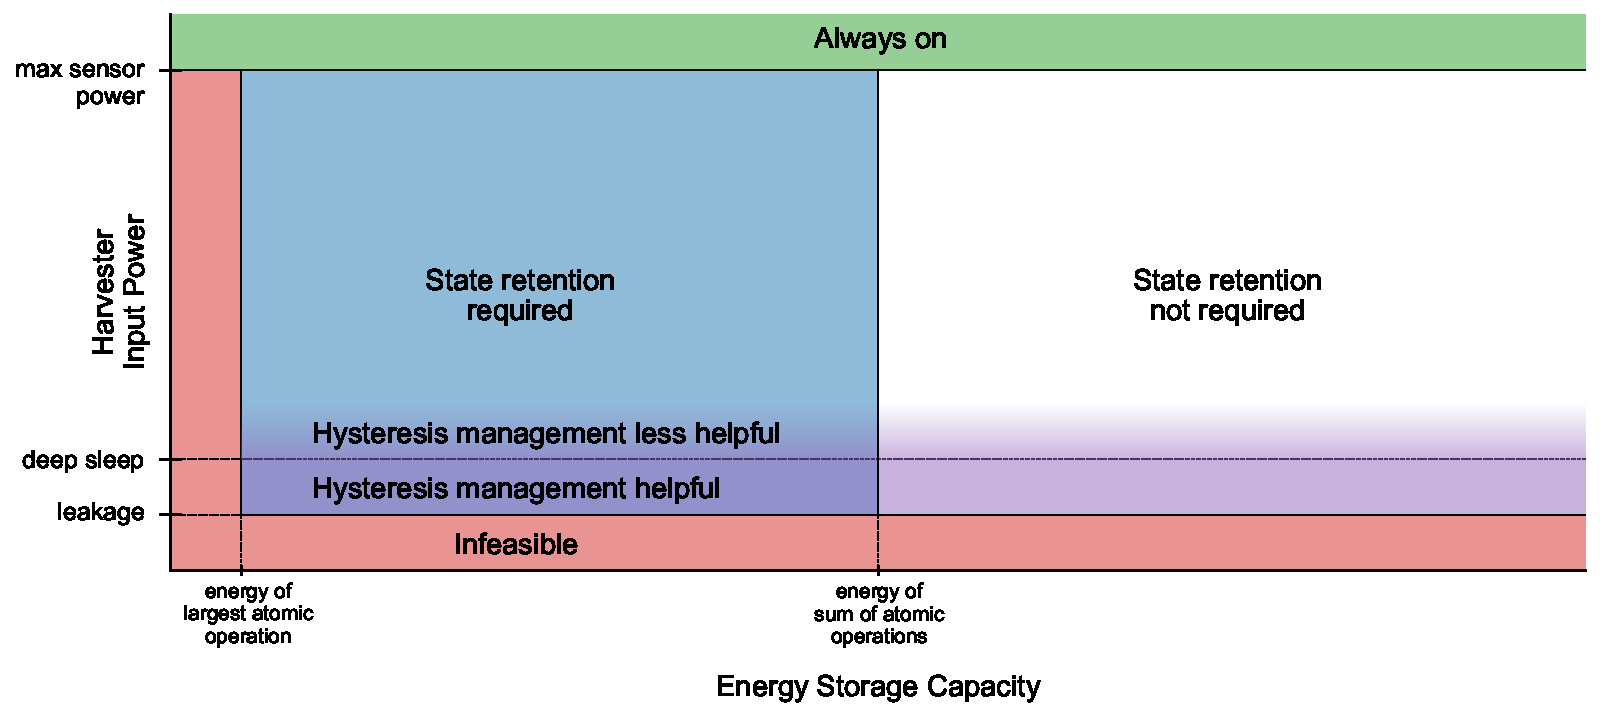
\includegraphics[width=\columnwidth]{figs/capacity/harvesting_framework/framework}
  \caption{
  %energy-harvesting
  %sensors have different capabilities and requirements
  \normalfont Design space for energy-harvesting sensors based on their energy
  income (which we assume is constant for this analysis), energy storage capacity, and workload.
  Workload is represented by the largest atomic/non-atomic operations supported
  by a design, as well as the deep sleep and leakage power.  The plot breaks
  into four regions: \textbf{1)} always
  on or effectively powered, \textbf{2)} Infeasible due to lack of energy storage or
  leakage higher than harvesting rate \textbf{3)} Feasible but requires checkpointing
  to make forward progress, and \textbf{4)} Enough energy storage to not require
  or benefit from checkpointing. Additionally, sensors which have high
  power when they enter deep sleep before depleting their
  energy buffer may benefit from hysteresis management techniques.
  This benefit diminishes with lower sleep currents and higher harvesting potential.
  %With increased capacity, sensors can avoid the complexity of intermittent
  %programming techniques and specialized, reconfigurable power supplies in addition
  %to the other benefits of increased capacity discussed
  %in \cref{sec:store}.
  }
\end{definefigure}


\begin{definefigure}{fig:intuition:eh_worth_it}
  \centering
  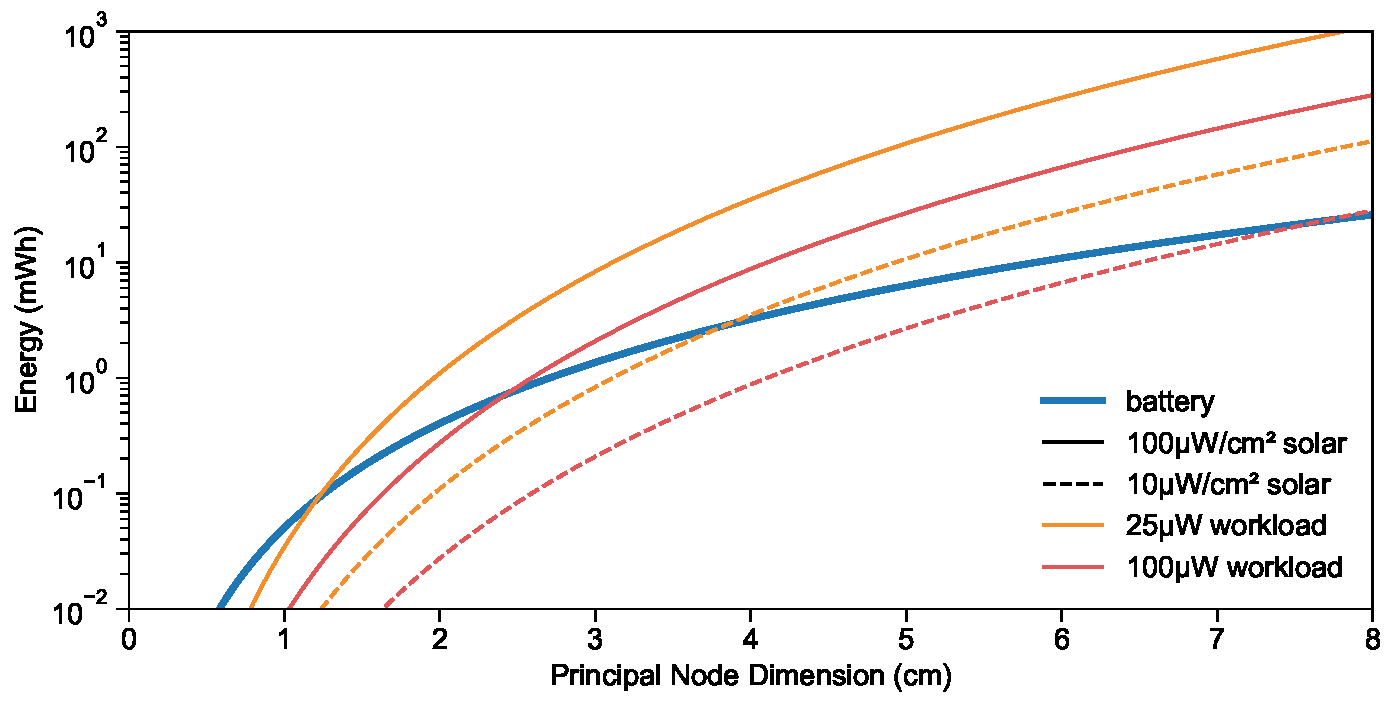
\includegraphics[width=\columnwidth]{figs/is_eh_worth_it_micro.pdf}
  \caption{
  A comparison of preallocated energy and captured energy. Note the logarithmic y-axis scale.
  This figure compares the energy offered by a cubic battery with that of potential harvestable energy captured by a square photovoltaic over the lifetime of the battery. 
  %The lifetime of the battery depends on different workloads, 
  %here represented by the orange (average 25\si{\micro\watt}) and red (100\si{\micro\watt}) lines. 
  %A solar cell accumulates energy over that same lifetime under different harvesting conditions, represented by a solid line 
  %(100\si[per-mode=symbol]{\micro\watt\per\centi\meter\squared}) or dashed line
  %(10\si[per-mode=symbol]{\micro\watt\per\centi\meter\squared}).
  %The point at which the harvesting lines (orange, red) cross the battery line (blue) indicate the size at which a similarly sized photovoltaic will harvest the same amount of energy provided by a similar sized battery over its lifetime. 
  At a sufficient size and in sufficient harvesting conditions, while powering an appropriate workload, solar energy-harvesting can provide more energy over the same time frame as a lithium battery.
  }
\end{definefigure}

\begin{definefigure}{fig:intuition:eh_worth_it_nano}
  \centering
  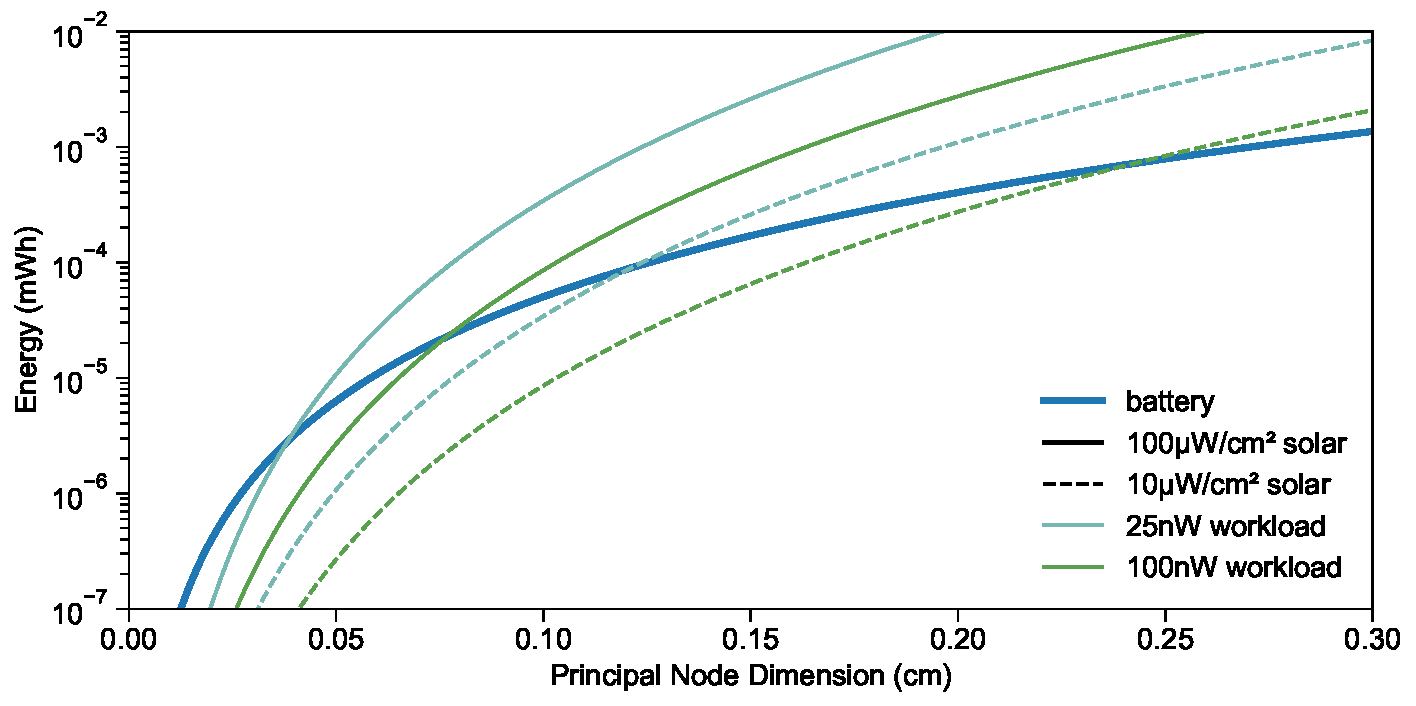
\includegraphics[width=\columnwidth]{figs/is_eh_worth_it_nano.pdf}
  \caption{
  A comparison of preallocated energy and captured energy for \si{\nano\watt} applications. 
  This figure is identical to \cref{fig:intuition:eh_worth_it} except that it considers the \si{\nano\watt} workloads that characterize millimeter-scale systems.
  A principle node dimension on the order of 1-2\si{\milli\meter} is generally sufficient for energy harvesting to collect more energy over a battery, in all but the worst case: a heavier workload with low harvesting potential.
  }
\end{definefigure}


\begin{definefigure}{fig:intuition:compound}
  \centering
  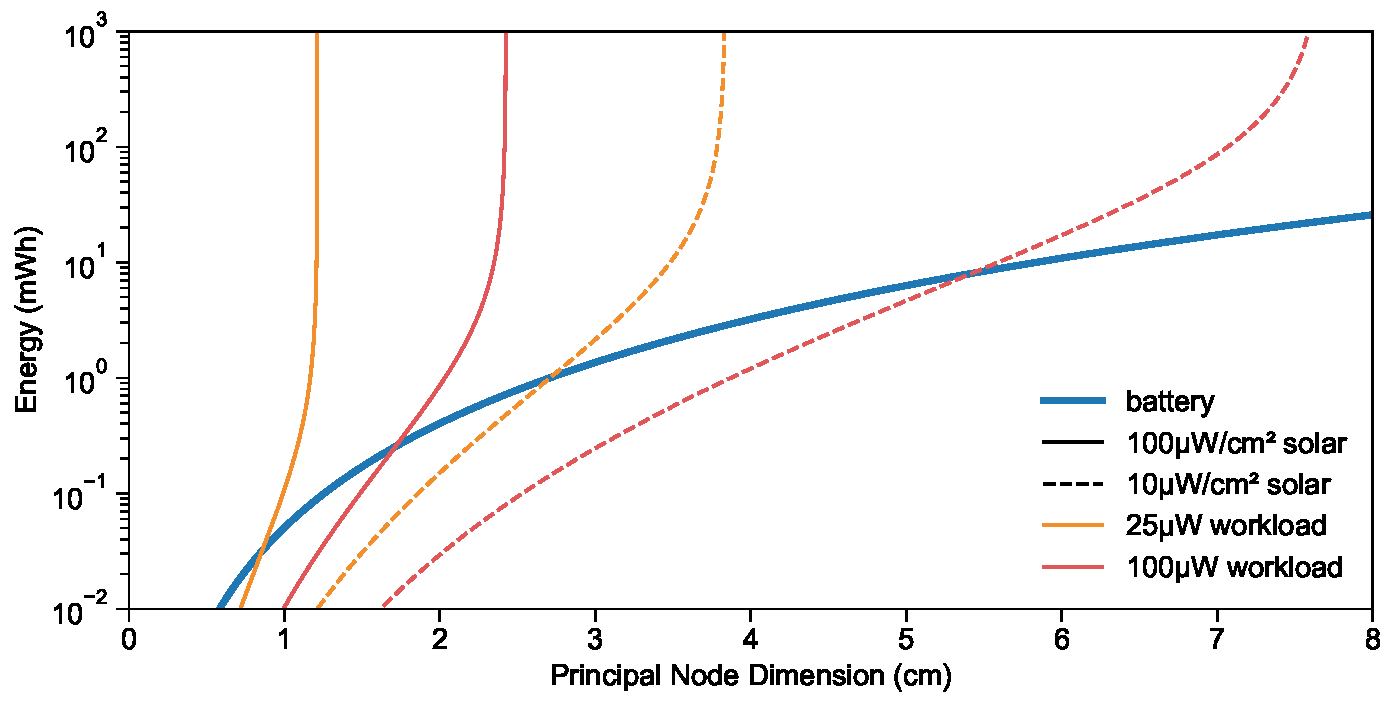
\includegraphics[width=\columnwidth]{figs/is_eh_worth_it_micro_compound.pdf}
  \caption{
    The energy captured by a hybrid system utilizing both harvesting and backup preallocated energy. This figure uses the same scale and line types as \cref{fig:intuition:eh_worth_it}. The addition of energy harvesting to a primary cell system has a compounding effect on lifetime and harvested energy. More harvested energy results in a prolongation of the lifetime of the primary cell. Subsequently, this lifetime extension results in an increase in harvested energy. 
    Because of the increased energy and battery lifetime, the crossing points now shift to the left in the figure, allowing a reduction in volume and area required for a battery and harvester, respectively. 
  }
\end{definefigure}
\chapter[A Simulation-based Exploration of Capacity][A Simulation-based Exploration of Capacity]{A Simulation-based\\Exploration of Capacity}
\label{chap:capacity}
In the previous chapter, we presented a simple model for energy capacity and explored the effect of capacity on the energy captured by a system. 
We utilized synthesized energy harvesting traces from an existing irradiance trace dataset, however we simplified the analysis by assuming a static average workload power.
This chapter will explore expanding our model to an energy state simulator for wireless sensors.
This simulator will utilize several different dynamic workloads based on benchmarks of real hardware, as well as considering a wireless sensor state machine that better models the behavior of a real sensor.
The rest of the chapter is an analysis of the performance of these simulated wireless sensor workloads under measured harvesting conditions.

\section{Upgrading Our Model}
\label{sec:capacity:modelling}
%The model and analysis we presented in \cref{sec:intuition:capacity} does not consider
%workload variability, and simplifies workload to an average.
In \cref{sec:intuition:capacity}, we argued that a sensor workload, which is often periodic or event driven, does not vary significantly beyond a few hours to a day of operation when compared to the variability of energy harvesting income. 
%Photovoltaic harvesting can vary significantly over the course of a day and throughout a year. 
To verify this assumption and expand our analysis of capacity, we seek to to explore the dynamic effects that energy
capacity and backup storage have on sensor performance in the face of workload variability.
We use representative energy harvesting traces, measurements of real hardware,
and synthesized dynamic workloads in a new model based on a simple wireless sensor state machine.
We use this model to simulate
the behavior of energy harvesting sensors. 
From the input traces of workload and energy harvesting income, our model produces estimates of sensor energy utilization, availability, responsiveness, and lifetime.

\placefigure{tab:capacity:rep}

\subsection{Energy Harvesting Income}
As in \cref{sec:intuition:capacity}, we utilize the EnHANTs irradiance trace dataset as energy income for our simulation.
Unlike our previous analysis, we do not use synthesized traces, and instead utilize the traces directly.
We choose to narrow our focus to two of the traces that we think most accurately represent indoor lighting conditions: Setup A and Setup D.
As shown in \cref{fig:intuition:traces}, Setup A represents a location that receives some sunlight but is mostly lit by artificial sources while Setup D represents a location near a window that receives significant light during part of the year.
Beyond \cref{fig:intuition:traces}, these traces are summarized in \cref{tab:capacity:rep}.
On average, Setup A provides an average of 15.1\ssi[per-mode=symbol]{\micro\watt\per\centi\meter\squared} which is on the lower end of expected irradiance in indoor environments. Setup D represents the higher end of indoor irradiance with an average 97.4\ssi[per-mode=symbol]{\micro\watt\per\centi\meter\squared}.

\subsection{Representative Hardware}
We limit our analysis to the effects of capacity,
independent of the differences of energy intensity or efficiency in device
component selection. To do so, we define an example photovoltaic energy harvesting
sensor platform that utilizes currently available commercial
components. These components are listed in \cref{tab:capacity:components}.
We choose new
components in an attempt to better represent prior energy storage designs and
give them the benefit of the improvements that have occurred in recent years.
We take benchmark
measurements of various tasks performed by this representative platform, such as the
amount of time and energy required to sample a sensor or send a Bluetooth Low
Energy (BLE) packet. 
These benchmarks are used to generate energy utilization metrics
for our representative workloads shown in \cref{tab:capacity:rep}.
The physical size of the solar panel used by this sensor
is assumed to be
10.9~cm\textsuperscript{2} and the volume of the sensor node is similar to prior
work like the Hamilton sensor~\cite{kim2018system}.
%We implement this design and describe it further in \cref{sec:impl:permamote}.

\placefigure{tab:capacity:components}

\subsection{Representative Workloads}
We find that sensing workloads generally fall into three
categories: (i) periodic sense-and-send~\cite{mainwaring2002wireless}, (ii) reactive event detection~\cite{campbellEnergy14,afanasov2020battery}, and (iii) infrequent,
long-running, high-energy events~\cite{levis2004trickle}. 
All of these workloads are characterized by long periods in which a sensor is inactive, punctuated by active events, which may be periodic or drawn from a probability distribution.
These active events may correspond to collecting a measurement from a sensor, performing some computation, and transmitting the results.
We choose a representative workload for each
of the three categories to use in our model.
We characterize our ``periodic sense-and-send''
workload as periodically sampling a light and three channel color sensor and sending a
BLE advertisement containing the data.
Our ``reactive workload'' consists of sending a BLE advertisement upon motion detection of the main
entrance of a university building, and we linearly scale the frequency
of these events to create synthetic traces with varying amounts of usage. 
We treat these workloads as atomic. 
When a measurement is taken or a packet is sent in response to a periodic schedule or a detected event, the energy spent on those operations must be spent instantaneously and atomically. 
This means a sensor must currently have sufficient energy stored to complete the operation, otherwise the event is considered ``missed'' and counted against the availability of the system.
Finally, our ``infrequent expensive'' workload is a
contiguous
task that is representative of an
over-the-air firmware update, which is randomly executed with an average occurrence rate
of once every two weeks.
We optimistically assume this long running task can be interrupted
and resumed at any point during execution and that any checkpointing does not incur any overhead.

\placefigure[t]{tab:capacity:parameters}

\section{An Energy Model for Wireless Sensors}
We use the previously discussed indoor irradiance traces, generalized
workloads, and hardware characterizations to model the behavior of sensors
using different types and sizes of energy storage. We develop an open
source\footnote{\url{https://github.com/lab11/permamote/tree/master/simulator}}
iterative simulator that allows parameterization of various system
characteristics, including regulator efficiency, solar harvester size
and efficiency, energy storage capacity, leakage, equivalent series resistance (ESR), and charge-discharge
efficiency. A subset of these parameters are summarized in \cref{tab:capacity:parameters}.

The simulation of our model operates as a second-by-second calculation of the
energy entering and exiting a device, similar to the model presented in \cref{sec:intuition:capacity}.
At every step, the simulation calculates the net energy gain or loss of the
system based on its current state, the instantaneous harvestable energy, and available stored energy.  
Occasionally,
the model performs a workload event based on either a periodic schedule (in the
case of a sense-and-send workload) or from a random distribution (reactive
event detection or a high-energy event). For our modeling, workload schedules
are generated from values listed in \cref{tab:capacity:rep}.
This simulation is performed for the entirety of an
input irradiance trace, which constitutes about a year of data. During
a simulation, metrics such as energy utilization, the fraction of completed
events versus expected events, and event time to completion are collected,
and if applicable, the primary-cell lifetime is estimated from a 
calculation of the net difference in energy in the system from the start to the end of the simulation, if negative. 

\placefigure{fig:capacity:statemachine}

During simulation, modeled devices can be online or offline and idle or performing
work. These states are shown in \cref{fig:capacity:statemachine}.  A device's state
transitions from top to bottom of this figure and vice versa depending on the
energy state of the secondary storage.
If the secondary-cell energy state drops below \texttt{min\_hyst},
the state of the system moves to the upper
half (\textsf{offline}) of this diagram. The state of the system moves downward (\textsf{online})
if the state of charge of the secondary reaches the \texttt{max\_hyst}
limit. 
Secondary charging hysteresis limits are defined by parameters described in \cref{tab:capacity:parameters}.
A device's state can also move
to the right or left of the state machine depending on whether a workload event
is scheduled, or the prescribed workload has been completed. A new
workload event is counted as failed if the device is not in the \textsf{Online
Idle} state when it begins.
In the case of the ``atomic''
sense-and-send and reactive workloads, the modeled device will only begin
to perform an expected workload event if it has
enough energy to perform the event in entirety. If the workload is not atomic,
the device will only begin scheduled work if it has enough energy to make the
configured minimum amount of progress. We
make an assumption that the duration of atomic events are less than the one
second simulation step.
We also assume that a modeled sensor has perfect, zero-energy progress
latching and can go to sleep at any point after an active event. 
If there is energy remaining after performing a task, the modeled sensor will
attempt to spend the rest of the simulation period in the \textsf{Online Idle} state.

If the simulated device is configured with a backup primary-cell, offline
states transform to ``primary'' states in which the device remains on and
able to perform work, but charges energy usage to the primary storage instead
of the secondary. During these periods, the secondary cell continues charging
from harvested energy. Upon reaching the upper charging hysteresis
limit, the device returns to an online state, using energy stored in the
secondary.  If the primary storage is depleted, the simulation ends early.

\placefigure{fig:usage}

\section{Capacity Increases Energy Capture and Availability}
\label{sec:capacity:capture}

Using our simulator, we can confirm that the conclusions 
from \cref{sec:intuition:capacity}
regarding the relationship between energy capacity and energy capture. 
An increase in sensor energy capacity results in an increase in the capture of energy during periods of abundant harvestable energy.
This additional energy has the effect of increasing the availability of the sensor, as the buffer serves to average out times of energy insufficiency and excess.
Higher
The next few subsections explore the effect of capacity on energy utilization and sensor availability.

\subsection{Ambient Energy Utilization}
\label{sec:capacity:utilization}

Ambient energy is underutilized when it is not used to support the specified
sensing application. This may happen for two reasons: 1) 
the secondary
energy storage is full but energy is still available for harvesting, and 2) the
sensor performs work based on its energy state rather than its application
goals. The first scenario is common for energy harvesting systems
presented in prior work that charge up a capacitor and wait for an event
before sensing and sending, failing to capture all energy that may
have been harvested while their capacitor was full~\cite{campbellEnergy14, afanasov2020battery}.
For an example of the second scenario, consider opportunistic batteryless
systems that transmit a packet every time their energy storage capacitor
is full rather than saving this energy for use during periods of lower harvesting
potential~\cite{hesterFlicker17, colinReconfigurable18}. Another example of this are sensors in which the harvesting
rate is proportional to the sensed phenomena~\cite{debruin2013monjolo}.

To explore ambient energy utilization as a function of storage size, we
use our simulation of the charge-discharge patterns of idealized energy stores under
the harvesting conditions and workloads described in \cref{sec:capacity:modelling}.
We perform multiple simulation runs while sweeping energy storage capacity and measuring the amount of harvestable energy captured and used by the intended workload.
We desire to isolate the effect of capacity from the type of storage, so the
idealized energy storage is assumed to have no leakage or ESR. 
%Our simulator is capable of considering these sources of inefficiency. 
%However, leakage and ESR are more dependent on the type of energy storage than the capacity, 
%making a sweep through capacity more complex than necessary when considering them.
This modeling is primarily accounting for our first classification of
wasted energy, since our workload definitions \textit{do not} perform
tasks in response to available energy; instead they attempt to maximize the success
rates for the specified sensing tasks.
The results of this modeling are shown in \cref{fig:usage}.
The x-axis of \cref{fig:usage} is split by energy capacities possible with capacitors, supercapacitors, and
batteries. 
The upper extents of capacity for capacitors represents ten 100\,\si{\micro\farad} tantalum capacitors~\cite{tantalumDatasheet}. 
For supercapacitors, the extent is represented by one
large 220\,mF supercapacitor~\cite{murataCap}. 
These delineations are not hard partitions, as capacitors and supercapacitors have a wide range of capacities and the capacities offered can overlap in some configurations.

Regardless of the amount of available energy or the workload considered, energy utilization increases as
buffer energy capacity increases. 
For scenarios with low harvesting potential and high
power workloads, a sensor with at least 1--10\ssi{\milli\Wh} of storage can accomplish 100\% utilization.
In cases of
high harvesting potential and low power workloads, utilization often
stops increasing before reaching 100\%. This
can be attributed to a small fraction of the available energy being sufficient
to fully support the sensing task.
For the low light, 15\ssi[per-mode=symbol]{\micro\watt\per\centi\meter\squared}, environment, a few of the workloads are eventually able to harvest 100\% of the available light as capacity increases. This indicates that the sensor performance is bounded by available harvestable energy, which is not enough to sustain the workload.
Conversely, in the high light 97\ssi[per-mode=symbol]{\micro\watt\per\centi\meter\squared} environment, regardless of the workload, the simulated sensors are not harvesting all or even the majority of the available energy. 
This indicates they are harvesting as much as needed to power their workload. 

In most cases, energy utilization for a workload is maximized with the energy capacity offered by small batteries or very large supercapacitors (\textgreater 1\ssi{\farad}).
A system configured with ceramic or tantalum capacitors will be unable to fully utilize available harvestable energy, resulting not only in unreliable energy, but also less energy. 
A capacitor-based batteryless system will simply harvest less overall energy than a supercapacitor or battery counterpart. 

\placefigure{fig:capacity:availability}
\placefigure{fig:capacity:period}

\subsection{Workload Availability}
\label{sec:capacity:availability}

The amount of captured energy directly impacts the capability of an energy harvesting sensor. With more captured energy, a system is better able to complete its workload consistently and with high reliability. 
We utilize our simulation to also measure the ability of varying energy capacity sizes to meet the simulated 
sensing tasks under various harvesting intensities. 
The results are
presented in \cref{fig:capacity:availability}. 
Similar to the results of \cref{fig:capacity:availability}, we see marked
increases in performance when the energy capacity is increased to 1--10\,mWh
of capacity.
Simulations experience 100\% availability for all but
the most energy constrained scenarios with high power workloads and
$\geq$2\,mWh of energy storage.
\Cref{fig:capacity:period} is another perspective of availability, and examines sweeping the period of the periodic workload with four decades of energy capacity.
These simulated results indicate that even 
with gratuitous energy harvesting potentials and infrequent workloads, sensors with energy capacity on the order of that offered by capacitors or supercapacitors will experience low availability compared to a sensor designed with sufficient energy capacity.
This is because they are
unable to capture and utilize enough harvestable energy to allow continuous sensing through periods with little to no harvestable energy, like nighttime or winter. 

\subsection{Workload Timeliness}
\placefigure{fig:capacity:ttc}
Finally, we analyze the ability of different storage configurations to perform a 
long-running, contiguous, higher energy task. 
The characteristics of the long-running task are presented in \cref{tab:capacity:rep_work}. We 
This long-running task is an example of a medium-sized, 50\ssi{\kilo\byte} over-the-air code update.
\Cref{fig:capacity:ttc} is a CDF of the time-to-completion for this update with different configurations of energy capacity, workload, and harvesting conditions.
Nearly all of the configurations with
0.28\,mWh of energy storage can complete the task in the minimum amount of time (5\,s). In comparison,
even reducing the energy storage size to match the energy
required for an update causes significant latency. 
Many of the updates for smaller energy storage configurations
do not complete for 1000-10,000\,s.
This aligns with the amount of time a sensor may sit
idle overnight waiting for power from daytime to continue and eventually complete its update.



% Mayfly/Flicker
% - Timekeeper: 1 10uF 0805YD106KAT2A 0.09 @ 100 (equiv 0.03 @ 100) (0.023)
% - MCU: 1 22uF Not specified, but an AVX 1210 costs 0.44 @ 100 (equiv 0.079 @ 100) (0.025)
% - Acel 1 2.2uF EMK107BJ225KA-T 0.039 @ 100 (equiv 0.036 @ 100) (0.015)
% - BLE  1 47uF GRM31CR60J476ME 0.21 @ 100 (equiv 0.16 @ 100) (0.028)
% - HUM  1 15uF C2012X7S1A156M125AC 0.37 @ 100 (equiv 0.19 @ 100) (0.052)
% - Press 1 33uF C3216X5R0J336M130AC 0.44 @ 100 (equiv 0.38 @ 100) (0.034)
%
% Capybara
% - test 1: 400uF ceramic (4x100 0.31 equive @100) (0.043), 330uF tant (0.69 equiv @100) (0.24), 67.5 mF super (?? $21?, $2.42)
% - test 2: 300uF ceramic (3x100), 1100uF tant ($2.43) (0.62), 7.5 mF super ($2.42) (
% - test 3: 300uF cerami (3x100)c, 100uF tant ($0.28) (0.17), 7.5 mF super ($2.42)
%
% Gecko Power Supply
% - 5 TLJG227M004R3000 1.39 @ 100 (0.37 equiv, 0.16 ali)
%
% Wisp
% - 1 10uF ?? $0.05 @ 100
\begin{definefigure}{fig:capacity:primary}
  \centering
  \begin{subfigure}{\columnwidth}
    \centering
    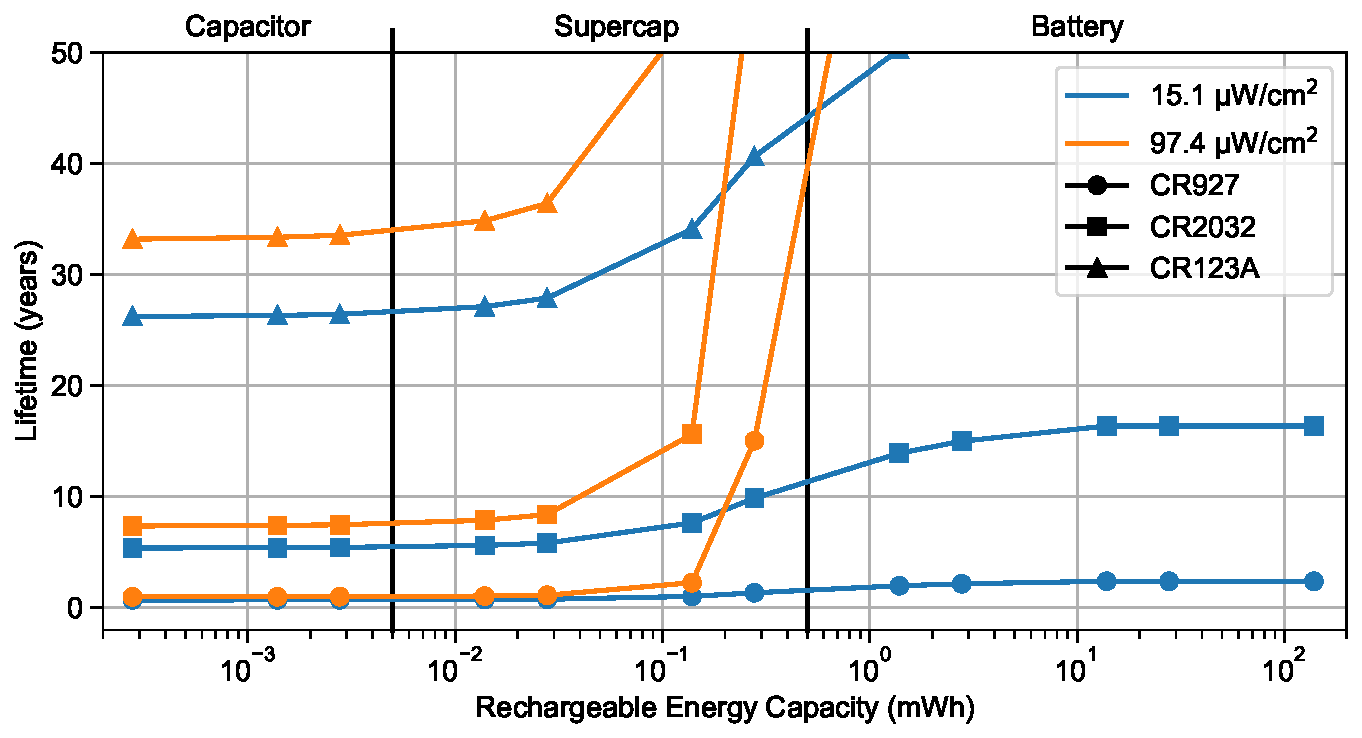
\includegraphics[width=\linewidth]{figs/capacity/primary/sense_and_send_life_vs_sec_size}
    \caption{Periodic Application}
    \label{fig:primary:sensesec}
  \end{subfigure}
  \begin{subfigure}{\columnwidth}
    \centering
    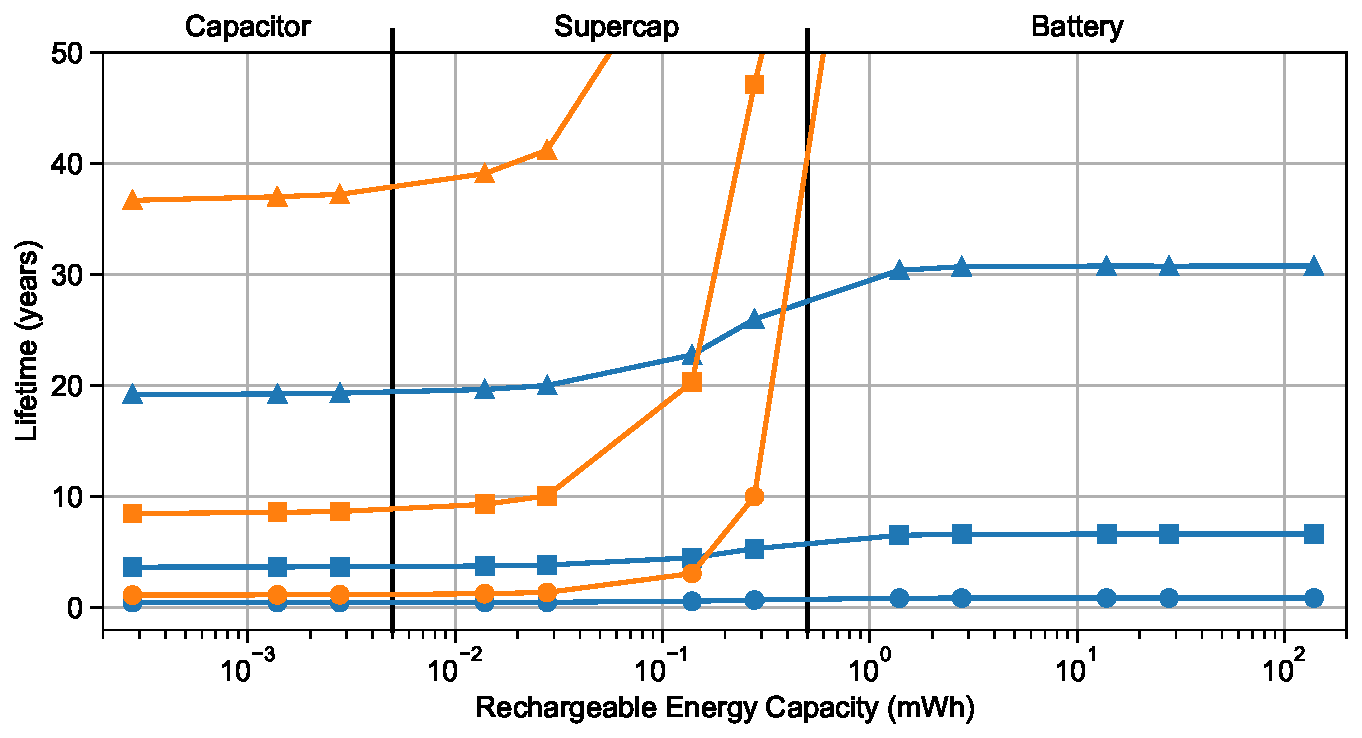
\includegraphics[width=\linewidth]{figs/capacity/primary/door_occu_life_vs_sec_size}
      \caption{Reactive Application}
    \label{fig:primary:eventsec}
  \end{subfigure}
  \caption{
    \normalfont
    Estimated lifetime
    when varying secondary energy capacity for different harvesting scenarios
    and backup energy storage sizes. 
    The periodic application's period
    is 30\,s and the reactive application events are scaled to
    represent a maximum of 2000 events per hour during the peak hour.
    %Harvesting scenarios and workloads
    %are described in \cref{sec:overview} and \cref{tab:capacity:rep}, and
    The backup
    sizes correspond to those found in common coin cell batteries:
    90\,mWh, 720\,mWh, 4500\,mWh for the CR927, CR2032, and CR123A respectively.
    As the ability to capture
    more harvested energy increases, the sensors lifetime increases.
    In some scenarios, expected
    lifetime becomes unbounded as the device is able to subsist entirely on harvested
    energy.
    %All scenarios experience substantial
    %increases in lifetime from increased secondary storage size.
    }
\end{definefigure}

\section{Availability Requires Backup}
\label{sec:capacity:primary}

Increasing secondary capacity greatly improves
availability across all workloads.
%for both periodic and reactive workloads.
However, some environmental
conditions and workloads do not reach 100\% availability regardless of the size
of the secondary store.
Some workloads simply require more energy
than is available to harvest, and cannot achieve high availability because they already capture all the energy they can.
%reactive workloads with large secondary
%capacities, some of the
For systems that can theoretically capture enough energy on average, they still may experience periods where they run out of stored energy.
Some of the results in \cref{fig:capacity:availability}
that appear to achieve near 100\% availability actually miss between 0.1 and 2\% of events because they did not initially start with enough energy stored.
%with
%diminishing returns for increased secondary capacity.
%Additionally, some workloads
In both of these cases, a backup energy store can greatly increase availability.
However, the introduction of a non-rechargeable backup means a system now has a finite lifetime.
%In both of these case, further increasing secondary
%capacity does not improve availability.
%and the desired application cannot rely soly on harvested power.
%and we expect that
%workloads which achieve slightly less than perfect availability are experiencing
%a combination of brief harvesting droughts and high amounts of temporally local activity
%that push the local average power well above that of the average harvested power.
While the second case may be solved with a sufficiently large secondary-cell that is deployed fully charged, the
diminishing returns of increasing secondary size and
unpredictability of some reactive applications
makes it difficult to rely solely on harvested power.

\placefigure{fig:capacity:primary}

We argue that 100\% availability is a significant improvement over
even low failure rates with respect to availability
%information
%for many applications
and simplicity due to the lack of intermittency.
%that is a consequence
%of availability.
As we discuss in \cref{sec:background:app}, many types of applications 
must provide high availability to be successful.
For applications that are human facing, research suggests that any unavailability
results in frustration and %lack of
unwillingness to adopt automated solutions~\cite{brushHome11, edwardsHome01, shehanHome07}.
To use energy harvesting sensors for human-facing applications, ones that control safety-critical systems, or applications that simply require consistent and periodic sensing, inherent unavailability is intolerable.
Beyond the availability of the normal sensor workload, it is also important to be able to detect and identify the failures in a sensor deployment.
Batteryless system failures are difficult to detect %and mitigate
because there is no method for differentiating between lack of energy
and an actual fault. While scheduled communication of current energy state
may help, this would be difficult for systems that only store enough
energy to perform a single operation~\cite{hesterFlicker17, yervaGrafting12, colinReconfigurable18,campbell2018energy}.
The only way to ensure there is \textit{always} energy available to issue a heartbeat message or report issues, a backup non-rechargeable source of energy is required.

%Finally, it is more difficult
%to program intermittent systems because programmers or the underlying
%programming model must monitor and adapt to available energy with fine
%granularity, both of which are non-trivial tasks.
%These systems have little ability to correct for failures
%even when they are detected.
%A reliable system has the ability to spend more short-term
%energy to correct for detected failures.

\subsection{Lifetime of a Backup Energy Store}
\label{sec:primary:lifetime}

To achieve 100\% availability and avoid frequent power and state loss,
designs can utilize a backup energy store.
In this section we simulate the workloads of energy harvesting sensors with backup non-rechargeable energy storage.
In instances where the rechargeable source is depleted, the system
can operate from the backup, masking the effects of variable energy income.
We estimate the lifetime of the backup based on the discharge rate resulting from the simulated workload. 
We consider a sensor's lifetime to be completed when its backup energy store is depleted.
We assume the backup energy store is  
a primary battery, as they offer very low self-discharge, long shelf life, and
superior energy density.

%that is pre-charged at the start of the
%node's life.
%This pre-charged energy store could be accomplished
%by either a large secondary-cell or a primary-cell, but to avoid increasing
%volume significantly this energy store will almost certainly manifest itself
%as a non-rechargeable battery.
An analysis of the reliable lifetime of sensors configured with energy
harvesting and a backup energy store is shown in \cref{fig:capacity:primary}.
%for
%both periodic and event based workloads.
We choose several backup energy
stores with energy equivalent to those found in several types of common
primary-cells. We see that with energy harvesting and a sufficiently
large secondary energy store, nodes can
achieve 100\% reliable lifetimes that exceed
what we can reasonably predict, especially for harvesting scenarios that
exceed the average power of the application. In these scenarios, 
the inclusion of a backup energy store is critical 
to ensure availability in uncharacteristically adverse conditions.
Even for conditions with
limited energy availability we still observe significant lifetime improvements
due to energy harvesting.
We identify a 2-4x increase in lifetime estimates from the smallest to largest
capacity simulated, if we only consider bounded results.
In some cases, lifetime estimates grow exponentially as rechargeable energy capacity is increased, indicating that with sufficient capacity and income, a workload almost never needs to utilize the energy in its non-rechargeable backup.
These results confirm the initial analysis performed in \cref{sec:intuition:hybrid}, which showed substantial lifetime improvements when considering hybrid energy harvesting systems with backup preallocated energy.
We emphasize that
these lifetime estimations are
just estimations, and while we do model the 1\,\%/year leakage
typical of coin cells, we do not consider the unknown
physical or chemical degradation that would be experienced over decades of use or in adverse environments.

\section{Summary}
In this chapter, we present an upgraded energy harvesting and storage model and use it to simulate the behavior and common workloads of wireless sensors.
This simulation improves upon the simple analysis performed in \cref{sec:intuition:capacity} by considering a dynamic workload, more realistic energy income and energy storage characteristics, and the effects of preallocated backup energy storage.
We use the results from multiple simulation runs to illustrate the impact of energy capacity on the performance of wireless sensors.
Increasing energy capacity allows a system to increase its energy utilization. In turn, increased energy utilization allows a wireless sensor to more successfully complete its workload, regardless of the type or distribution of workload activity.
When considering the workloads presented in \cref{sec:capacity:modelling} and the results of \cref{fig:usage,fig:capacity:availability}, they will require an energy buffer capacity on the order of 1--10\ssi{\milli\Wh} to achieve sufficient energy capture and workload availability.

Despite the improvements granted by increased capacity, a wireless energy harvesting sensor will still be limited by the magnitude of available harvestable energy.
In cases where harvestable energy is insufficient to power an intended application workload, it can be beneficial to include a backup non-rechargeable source of energy to ensure high availability.
While this inclusion results in a wireless sensor with a finite lifetime, energy harvesting with sufficient rechargeable energy capacity can significantly increase the system lifetime.

In the next chapter, we explore and compare the options for rechargeable energy capacity for wireless sensors, including capacitors, supercapacitors, and batteries. 
Capacitors and reasonably sized supercapacitors are unable to provide the energy capacity predicted by our workload simulations. 
However, batteries are a promising option to provide sufficient energy capacity and density to achieve the energy utilization and workload availability gains identified in this chapter.




\begin{definefigure*}{fig:usage}
  \centering
  \begin{subfigure}{\columnwidth}
    \centering
    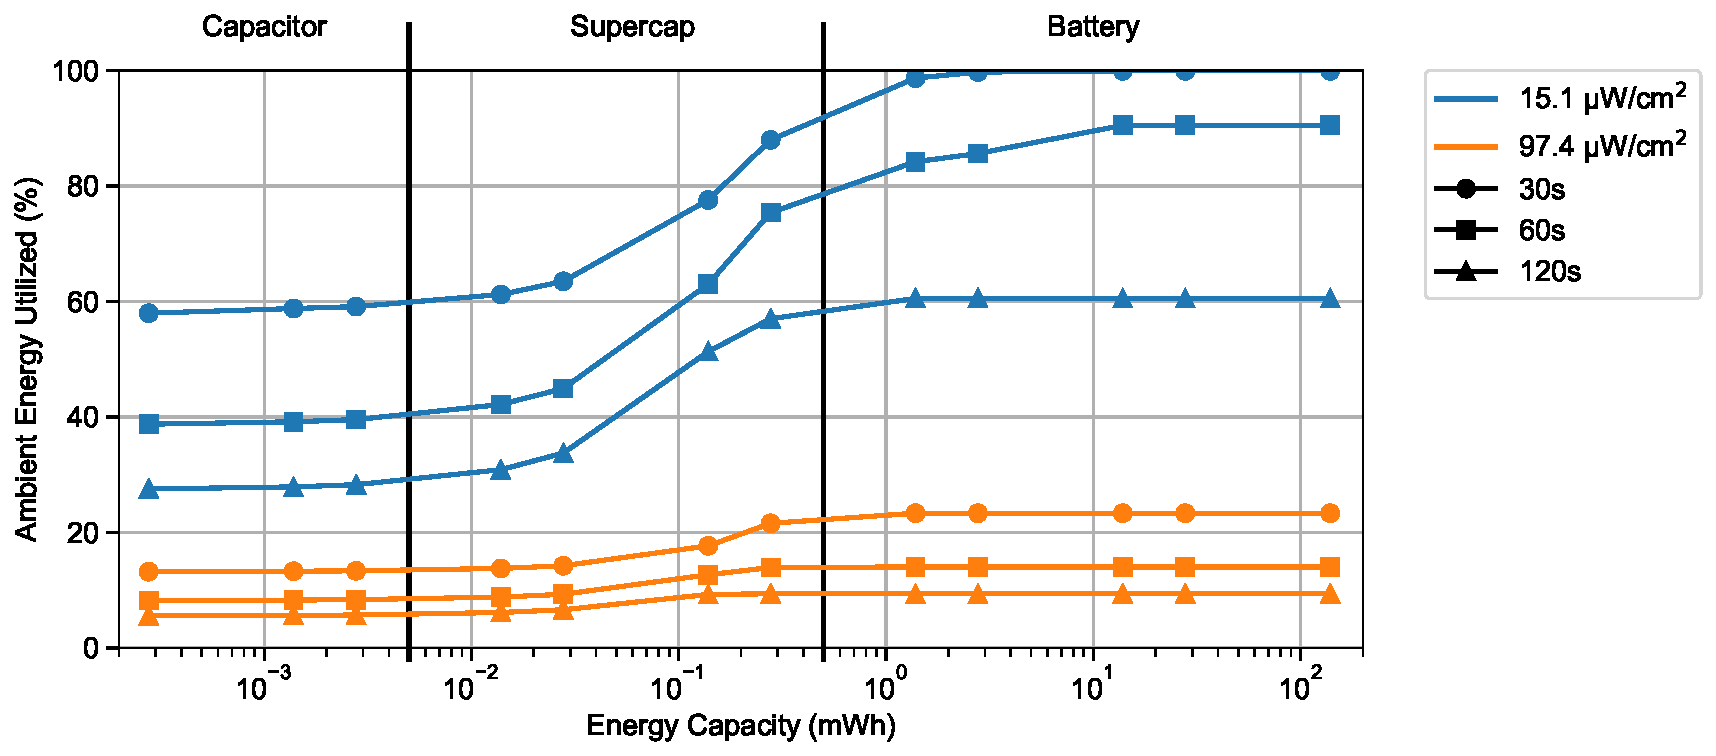
\includegraphics[width=\linewidth]{figs/capacity/sense_and_send/usage_reliability_v_secondary_capacity/usage_vs_secondary_size.pdf}
    \caption{Periodic application}
    \label{fig:usage:sensesec}
  \end{subfigure}
  \begin{subfigure}{\columnwidth}
    \centering
    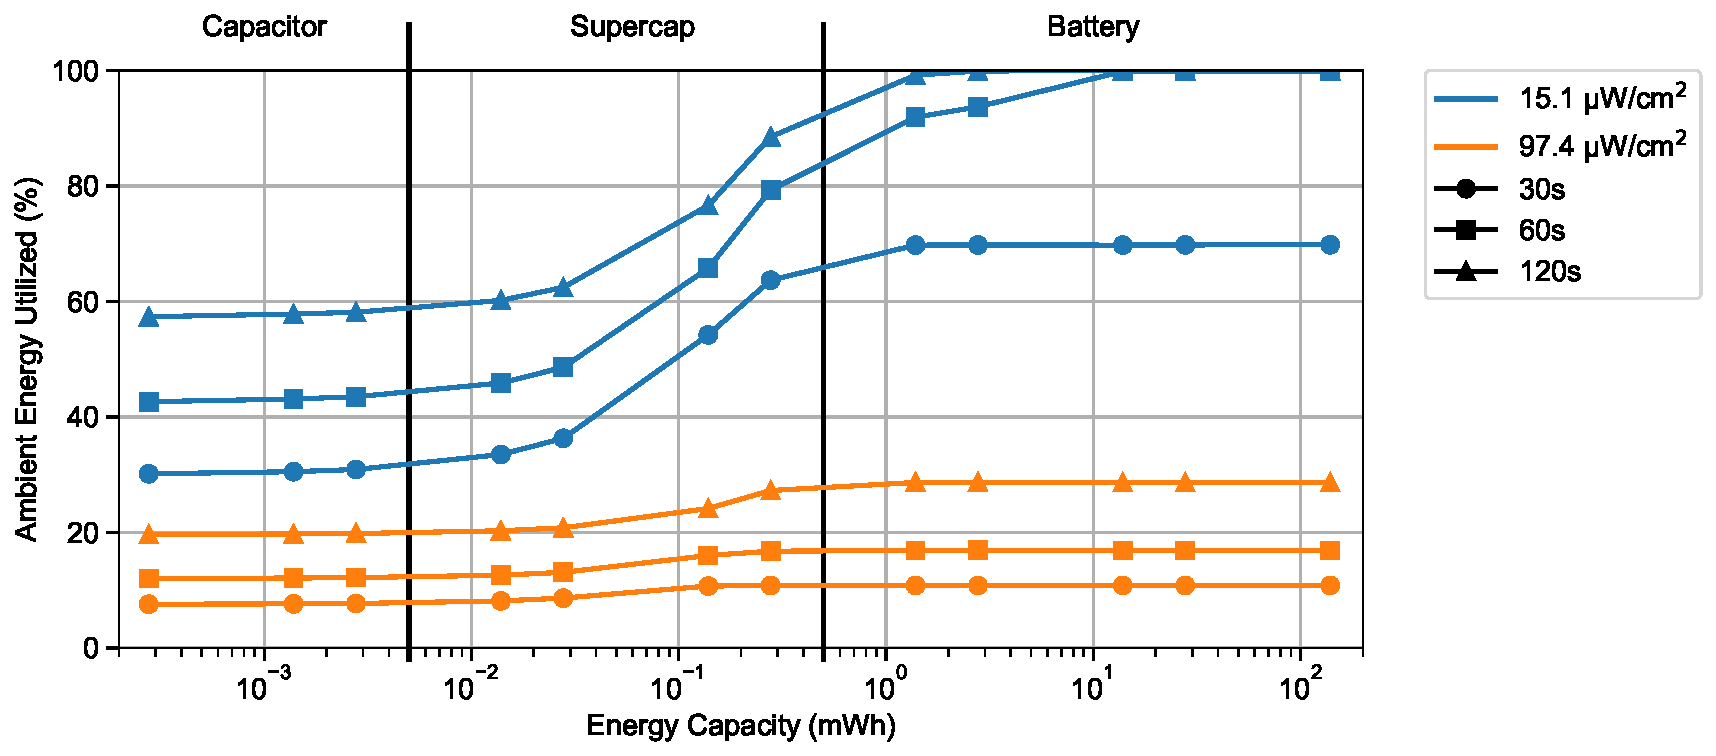
\includegraphics[width=\linewidth]{figs/capacity/door_occupancy/usage_vs_secondary_size}
    \caption{Reactive application}
    \label{fig:usage:eventsec}
  \end{subfigure}
  \caption{\normalfont Ambient energy utilization
    as a function of idealized secondary storage capacity for different
    harvesting scenarios and workloads. The harvesting scenarios and workloads
    are described in \cref{tab:capacity:rep}.
    \Cref{fig:usage:sensesec} represents the energy utilized by a periodic sense and send application, while \cref{fig:usage:eventsec} is the energy utilized by a event-driven application.
    Despite these two workloads exhibiting different event distributions and variance, the overall energy utilization follows the same trend with energy capacity. 
    As energy storage increases, the harvestable energy used in
    the application also increases. %implying
    %increased application performance.  
    Some scenarios, such as the periodic
    30\,s, 15.1\,\uW/cm\textsuperscript{2} case, reach 100\% utilization at
    sufficient secondary capacities indicating that all of the available energy is captured and may not
    be enough to meet the application's requirements.
    Generally, for both workloads and irradiance traces, from
    the smallest to largest capacity simulated, we see a 1.4-2.3x increase in
    utilized energy.
    }
\end{definefigure*}

\begin{definefigure*}{fig:capacity:availability}
  \centering
  \begin{subfigure}{\columnwidth}
    \centering
    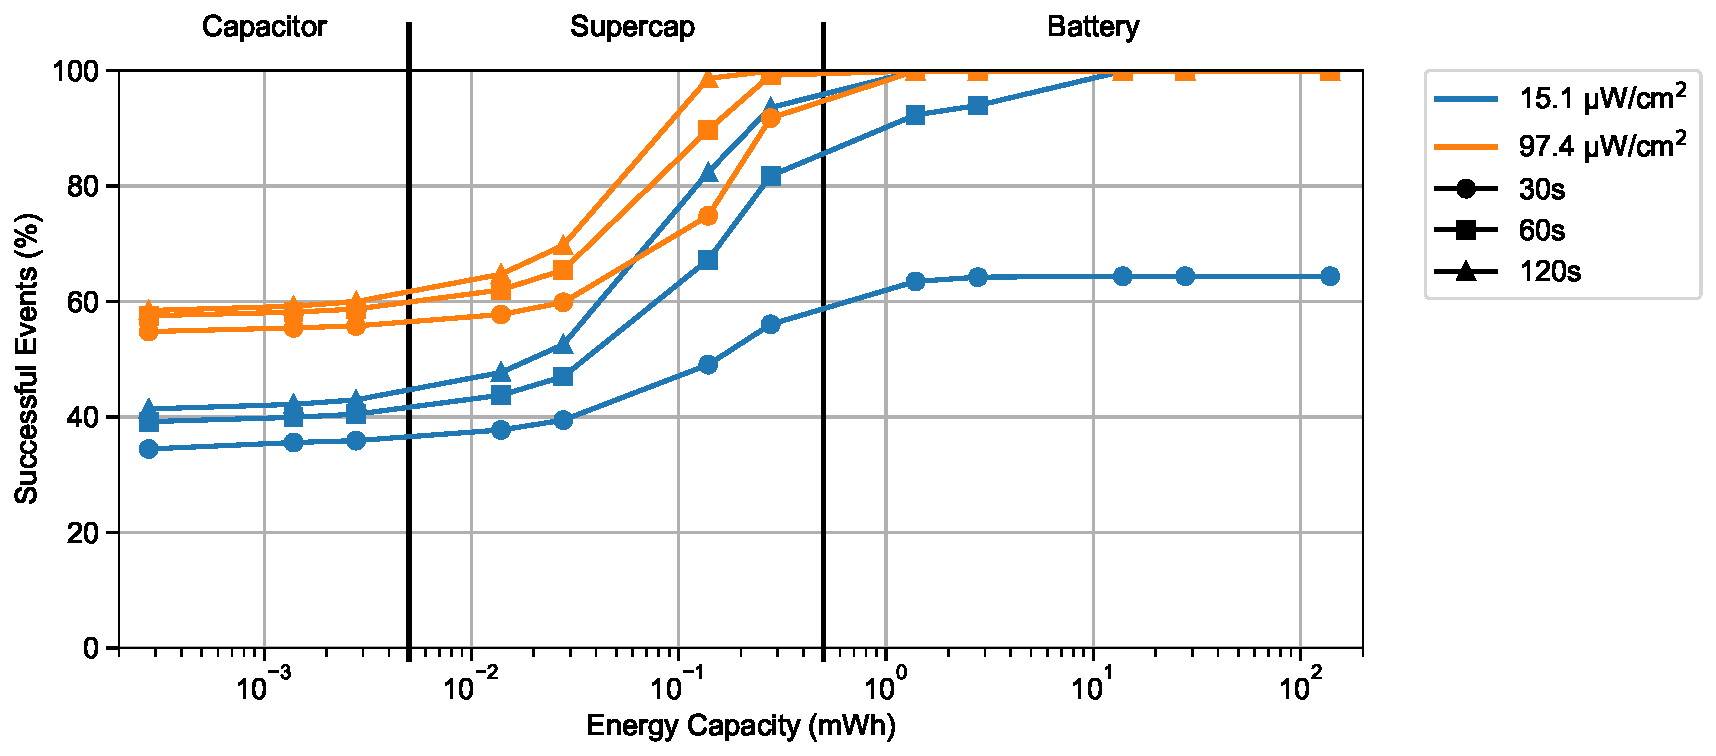
\includegraphics[width=\linewidth]{figs/capacity/sense_and_send/usage_reliability_v_secondary_capacity/events_vs_secondary_size.pdf}
      \caption{Periodic application}
    \label{fig:capacity:availability:sensesec}
  \end{subfigure}
  \begin{subfigure}{\columnwidth}
    \centering
    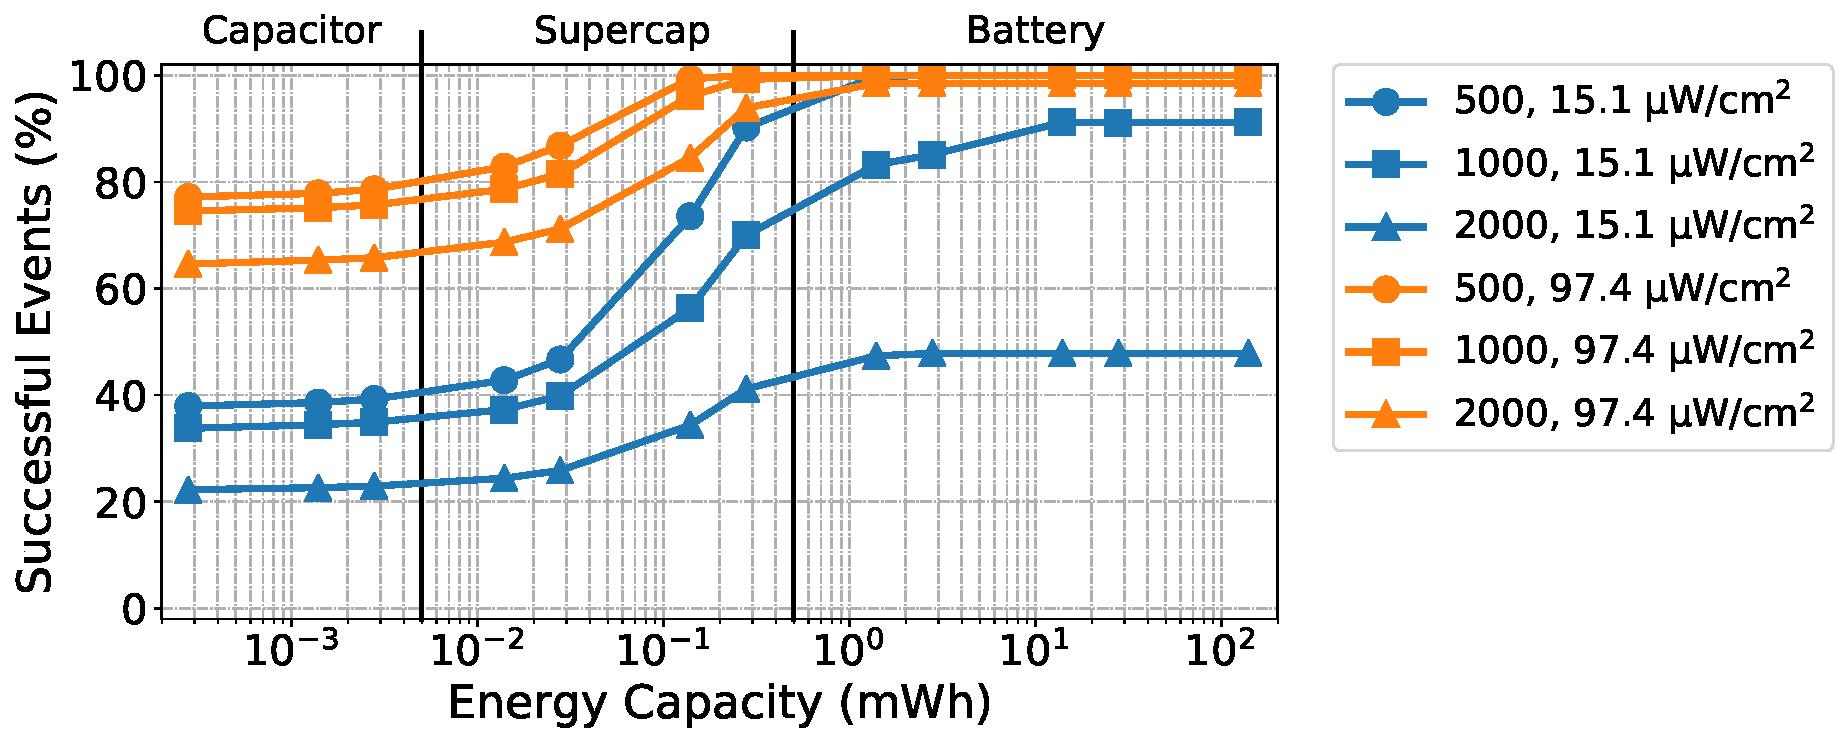
\includegraphics[width=\linewidth]{figs/capacity/door_occupancy/events_vs_secondary_size}
    \caption{Reactive application}
    \label{fig:capacity:availability:eventsec}
  \end{subfigure}
  \caption{
    \normalfont
    Workload availability
    for different harvesting scenarios, workloads, and idealized secondary storage sizes.
    We define availability as the percentage of successfully completed events. If a periodic or random event occurs and the sensor does not have sufficient energy to complete the event, that event is not completed and is considered missed.
    As expected, workload availability follows a similar 
    trend as energy utilization, improving with increased secondary energy
    storage and energy capture. 
    For both periodic and reactive workloads, from the smallest to
    largest capacity simulated, we see a 1.4-2.7x improvement in availability.
    In cases where average harvester power is sufficient to power the workload completely, the sensor achieves 100\% availability on the workload when configured with sufficient capacity.
    }
\end{definefigure*}

\begin{definefigure}{fig:capacity:period}
      \centering
      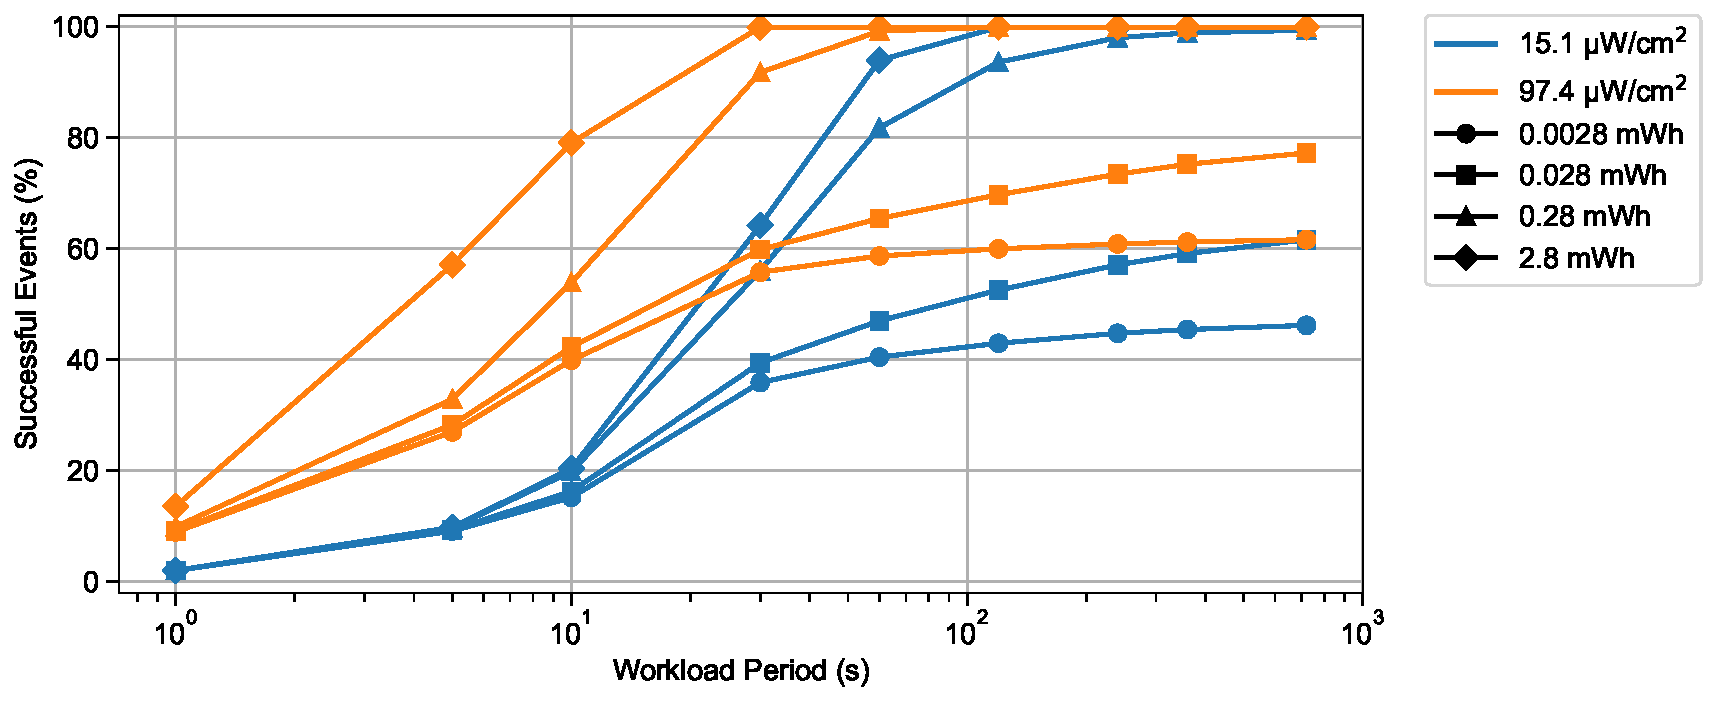
\includegraphics[width=\linewidth]{figs/capacity/sense_and_send/usage_reliability_v_period/events_vs_period.pdf}
    \caption{
    The performance of workloads with different periodicity with four decades of energy capacity.
    We investigate the period at which different secondary storage sizes
    meet a specific availability, showing that even with infrequent periodic
    workloads, small amounts of secondary storage have low availability while
    larger secondary stores approach 100\% availability. 
    } 
\end{definefigure}
    
\begin{definefigure}{fig:capacity:ttc}
      \centering
      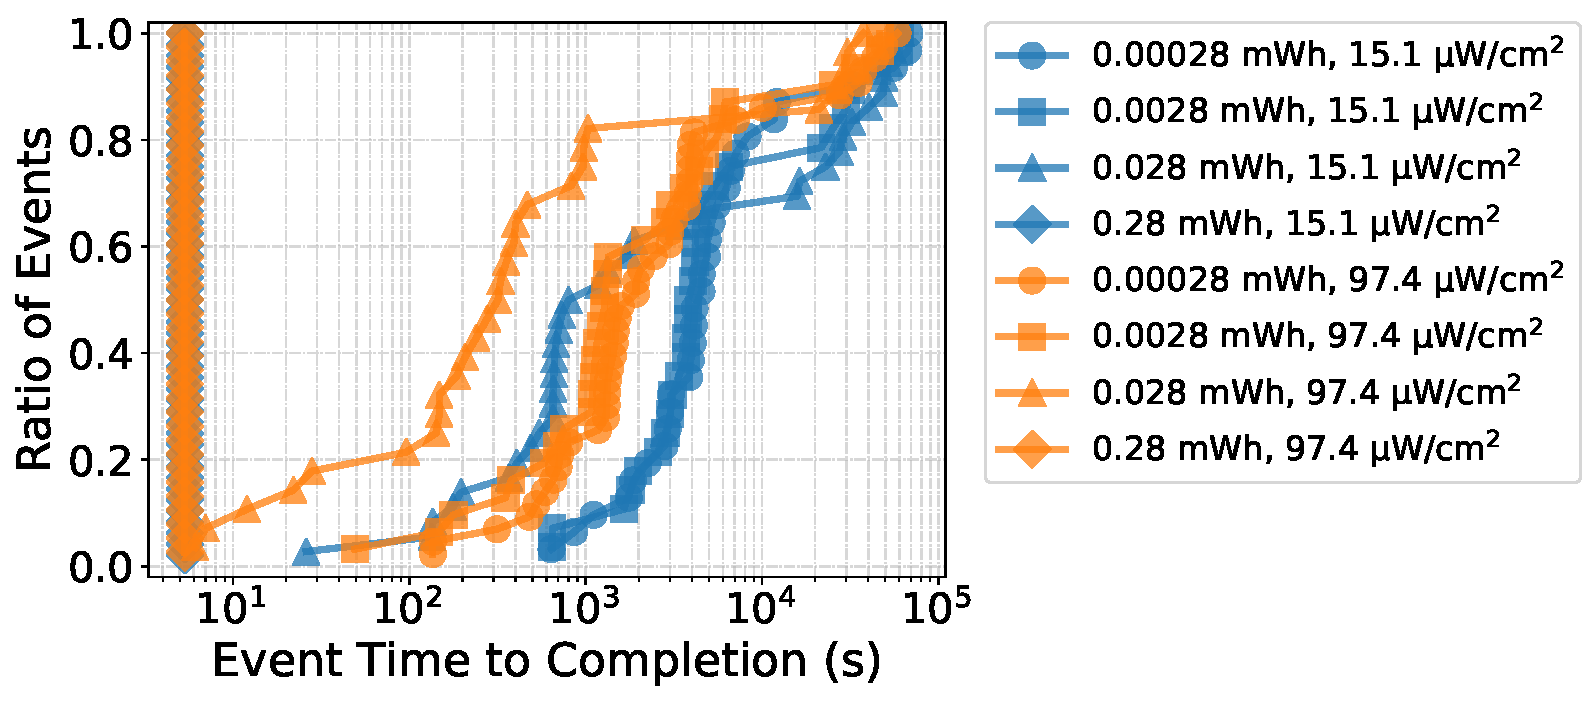
\includegraphics[width=\linewidth]{figs/capacity/ota_update/ttc_ota}
      \caption{
      A CDF of time to completion of a long-running, high energy event.
        In this
        workload, events are not atomic, and can be paused and resumed based on
        available energy. With secondary capacities that are large relative to the
        workload (which takes 93\,mJ) we see immediate completion.
        However, performing the event on smaller secondary capacities can take
        between three hours and a day to complete even for scenarios with large
        amounts of harvestable ambient energy.
      }
\end{definefigure}

\begin{definetable}{tab:capacity:rep}
    \begin{threeparttable}
    \centering
    \begin{subtable}{\columnwidth}
            \begin{tabularx}{\columnwidth}{@{\extracolsep{\fill}} l | c | c | c | c }
                Irradiance Trace  & Total Days & \thead{\\ Average Power\\(\textmu W/cm\textsuperscript{2})} & \thead{90\textsuperscript{th} Percentile\\Daily Power \\(\textmu W/cm\textsuperscript{2})} & \thead{10\textsuperscript{th} Percentile\\Daily Power \\(\textmu W/cm\textsuperscript{2})} \\\hline
                EnHANTs A   & 394  & 15.1     & 25.0      & 5.2\\
                EnHANTs D   & 311  & 97.4     & 256.5     & 24.8\\
                %Enhants C   & 327  & 745.4    & 1610.0    & 176.1\\
            \end{tabularx}
            \caption{Indoor photovoltaic irradiance traces}
            \label{tab:capacity:rep_trace}
        \end{subtable}\\
        \vspace{1em}
        \begin{subtable}{\columnwidth}
            \centering
            \begin{tabularx}{\columnwidth}{@{\extracolsep{\fill}} l | c | c | c }
                Workload Class & Energy per Event (uJ) & Average Period & Average Power (\textmu W)\,\tnote{a}\\\hline
            \multirow{4}{*}{Periodic}   & \multirow{4}{*}{586}  & 10\,s                 &  58.6     \\
                                        &                       & 30\,s                 &  24.5     \\
                                        &                       & 60\,s                 &  14.7     \\
                                        &                       & 120\,s                &  9.8      \\\hline
            \multirow{3}{*}{Reactive}   & \multirow{3}{*}{86}   & 3.4\,s\,\tnote{b}     &  25.3     \\
                                        &                       & 6.8\,s\,\tnote{b}     &  17.6     \\
                                        &                       & 13.6\,s\,\tnote{b}    &  11.3     \\\hline
                 Long-Running           & 93,300                 & 2\,weeks\,\tnote{c}  &  5.1      \\
            \end{tabularx}
            \caption{Representative workloads}
            \label{tab:capacity:rep_work}
        \end{subtable}
        \vspace{1em}
    \end{threeparttable}
    \small
    \begin{tablenotes}[para]
    \item[a] Average power includes an average 5\,\textmu W idle power, measured in \cref{sec:impl:permamote}.\\
    \item[b] Event times are based on a Poisson distribution for each hour of the day and drawn every second. The distribution is parameterized by collected entryway data then scaled.\\
    \item[c] Event time is based on a uniform distribution and drawn every second.
    \end{tablenotes}
    \caption{\normalfont Representative harvesting conditions and workloads.
    To evaluate different energy harvesting storage techniques, we define a set of energy harvesting
    conditions and workloads that are representative of common sensing applications. We choose two
    real irradiance traces with different magnitudes and distributions of available energy.
    These traces are summarized in \cref{tab:capacity:rep_trace}.
    We define three
    workloads: periodic, reactive, and long-running, and we characterize those workloads
    for different event frequencies. The energy used for each event is measured
    on our reference hardware described in \cref{sec:impl:permamote}.
    Statistics for the three workloads are described in \cref{tab:capacity:rep_work}.
    }
\end{definetable}

\begin{definetable}{tab:capacity:parameters}
    \centering
    \begin{tabularx}{\columnwidth}{@{\extracolsep{\fill}} lll}
\hline
\textbf{Config Type}& \multicolumn{1}{l}{\textbf{Parameter}}                   & \multicolumn{1}{l}{\textbf{Description}} \\ \hline
\textbf{Device}     & \texttt{operating\_voltage}                              & Output voltage of the power subsystem    \\
                    & \texttt{boost\_efficiency}                               & Efficiency of the boost converter        \\
                    & \texttt{frontend\_efficiency}                            & Efficiency of the harvesting frontend    \\ \hline
\textbf{Secondary}  & \texttt{capacity}                                        & Capacity of secondary in joules or mAh   \\
                    & \texttt{esr}                                             & Equivalent series resistance in ohms     \\
                    & \texttt{leakage\_constant}                               & Factor for capacity dependent leakage    \\
                    & \texttt{\string{max, min\string}\_hyst}                  & Secondary capacity upper/lower hysteresis\\ \hline
\textbf{Primary}    & \texttt{capacity}                                        & Capacity of primary in mAh               \\
                    & \texttt{leakage\_percent}                                & Percent capacity leakage per year        \\ \hline
        \textbf{Harvester}  & \texttt{area}                                    & Area of solar harvester in cm\textsuperscript{2}\\
\textbf{(Solar)}    & \texttt{efficiency}                                      & Efficiency of solar panel                \\ \hline
%\textbf{Workload}   & \texttt{type}                                            & Periodic or Reactive                     \\
%                    & \texttt{period/scale}                                    & Period, or scale for average \# of events \\
%                    & \texttt{opportunistic}                                   & Ignore period, and perform events ASAP   \\
%                    & \texttt{sleep\_current}                                  & Current draw of system in low power mode \\
%                    & \texttt{startup\_\string{energy, period\string}}         & Energy, time required for startup        \\
%                    & \texttt{event\_\string{energy, period\string}}           & Total energy, time required for work event \\
%                    & \texttt{atomic}                                          & Workload is atomic, or intermittent      \\
%                    & \texttt{event\_period\_min}                              & If not atomic, minimum splitable period  \\ \hline

    \end{tabularx}
    \caption{\normalfont Simulation configuration parameters.
      A subset of available configuration options for the sensor energy simulation. 
      Simulated sensors can be configured to use 
      secondary storage and an energy harvester, a
      primary-cell, or both. A secondary-cell can be configured with a
      hysteresis, with a lower bound set to \texttt{min\_hyst}
      and an upper bound of \texttt{max\_hyst}.
      %This upper bound must represent
      %the minimum amount of
      %energy to do useful work.
      %Therefore, the upper bound of charging
      %hysteresis is set to \texttt{secondary\_max\_hyst}.
      %Workloads are
      %configured to be either periodic or reactive, and workload intensity is
      %determined by period, or a scaling factor determining the average number
      %of events picked from a random distribution.
      }
\end{definetable}
\begin{definefigure}{fig:capacity:statemachine}
    \centering
    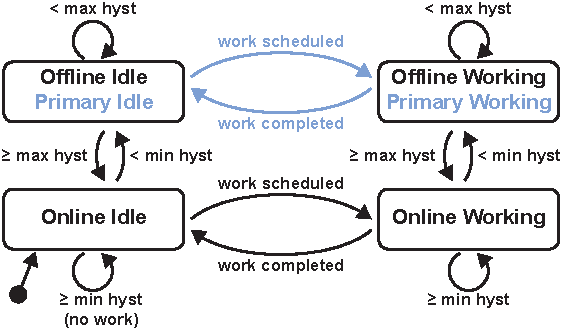
\includegraphics[width=\columnwidth]{figs/capacity/model_state_machine}
    \caption{\normalfont Model state machine.
    A modeled device can be in one of four states: \textsf{Offline Idle},
    \textsf{Online Idle}, \textsf{Online Working}, and \textsf{Offline
    Working}. When a device is \textsf{Offline Idle}, it has run out of energy
    and is off. If a device is \textsf{Online
    Idle}, it is on and in deep sleep, ready to perform work if triggered. If
    triggered, a device moves to \textsf{Online Working}, where it performs a
    portion of a work event.  If a workload is atomic, workload events
    \textit{must} be completed in one \textsf{Online Working} step, without any
    transitions to an offline state.  \textsf{Offline Working} means that while
    working on a non-atomic task, the device ran out of energy, checkpointed,
    and is waiting to harvest more and resume its task.  For devices
    configured with a primary-cell, \textsf{Offline Idle} and \textsf{Offline
    Working} become \textsf{\textcolor{primary-blue}{Primary Idle}} and
    \textsf{\textcolor{primary-blue}{Primary Working}} respectively.  In these
    states, outgoing energy is charged against the primary-cell and the device
    remains online and able to perform work for the life of the primary-cell.
    %State transitions are determined by incoming energy, the state of charge of
    %the secondary storage, and the generated work schedule from workload
    %parameters.
    }
\end{definefigure}

\begin{definetable}{tab:capacity:components}
    \begin{threeparttable}
    \centering
        \begin{tabularx}{\columnwidth}{@{\extracolsep{\fill}} l | l | c | c}
            Component                           &  Function                     & Active Power          & Idle Power \\\hline
            \multirow{2}{*}{Nordic NRF52840}    & Processor                     & 56\,\uA/MHz           & 940\,nA\,\tnote{a}  \\
                                                & Radio                         & 5.2\,mA @ 0\,dbm      & \textemdash\,\tnote{a}\\
            Ambiq AB1815-T3                     & Real time clock               & 55\,nA                & N/A\,\tnote{b}  \\
            ST Micro LIS2DW12                   & Accelerometer                 & 1\,uA @ 12.5\,Hz      & 50\,nA  \\
            Maxim MAX44009                      & Light sensor                  & 650\,nA               & N/A\,\tnote{b}  \\
            Intersil ISL29125                   & Color sensor                  & 56\,\uA               & 500\,nA  \\
            Silicon Labs SI7021                 & Humidty sensor& 1.5\,\uA @ 1\,Hz      & 60\,nA  \\
            TE Connectivity MS5637              & Pressure sensor               & 0.6 - 5\,\uA @ 1\,Hz  & 10\,nA  \\
            Panasonic EKMB11011                 & PIR Occupancy                 & 100\,\uA              & 1\,uA  \\
        \end{tabularx}
    \end{threeparttable}
    \begin{tablenotes}[para]
    \item[a] Sleep current for both processor and radio.
    \item[b] No shutdown or idle mode.
    \end{tablenotes}
    \caption{
    The components used by our representative hardware. Benchmarks of the processor, radio, and sensors presented here are used to establish our representative workloads used by our wireless sensor energy simulation.
    These components are among the lowest power options available, and
    are even 2-4x lower power than those used on relatively recent
    systems~\cite{hesterFlicker17,andersen2017hamilton,colinReconfigurable18}. 
    }
    %Technology
    %scaling for embedded sensors, processors, and radios
    %has driven down the average power of a sensor node much closer to the
    %harvestable solar energy available in indoor lighting conditions. This allows
    %more systems to subsist or achieve extended lifetimes through energy harvesting.
\end{definetable}


\chapter{A Quantitative Evaluation of Energy Storage}
\label{chap:battery}

From the previous two chapters, we have identified the value of properly sizing energy capacity in an energy harvesting design to increase energy capture and system availability. 
Many batteryless sensor designs have chosen to utilize capacitors in their designs, which severely limit energy capacity and the performance of the system. 
Many modern applications are attempting to push the energy bounds of sensing, computation and networking, and batteryless systems have begun incorporating supercapacitors to provide the necessary energy capacity to make certain applications feasible~\cite{nardello2019camaroptera}.
%Due to an increased need for energy storage to enable more advanced sensing and processing, the majority of modern batteryless research energy harvesting platforms utilize supercapacitors instead of tantalum or ceramic capacitors due to their superior energy density.
These designers have eschewed batteries as an option, despite their vastly superior energy density, dismissing them qualitatively as 
bulky~\cite{yervaGrafting12, hester2017future, hesterTragedy15, luciaIntermittent17, hesterFlicker17, hesterTimely17, colinReconfigurable18, yildirim2018ink, nardello2019camaroptera, geissdoerfer2019shepherd, majid2020continuous, shukla2019skinnypower},
inefficient~\cite{yervaGrafting12, luciaIntermittent17, nardello2019camaroptera, shukla2019skinnypower},
expensive~\cite{hester2017future, hesterTragedy15, hesterFlicker17, hesterTimely17, yildirim2018ink, majid2020continuous},
short-lived~\cite{hester2017future, hesterFlicker17, hesterTimely17, colinReconfigurable18, luciaIntermittent17, yervaGrafting12, shukla2019skinnypower, geissdoerfer2019shepherd, nardello2019camaroptera, fraternali2020ember, majid2020continuous}.
%high-maintenance~\cite{hesterNew17, hesterTragedy15, hesterFlicker17, hesterTimely17, colinReconfigurable18, luciaIntermittent17},
temperature-sensitive~\cite{hester2017future, hesterFlicker17, hesterTimely17, luciaIntermittent17, colinReconfigurable18},
%difficult to monitor~\cite{hesterNew17, hesterTragedy15, hesterFlicker17, hesterTimely17, colinReconfigurable18, luciaIntermittent17},
%fragile~\cite{hesterNew17, hesterTragedy15, hesterFlicker17, hesterTimely17},
and dangerous~\cite{hester2017future, hesterFlicker17, hesterTimely17,  yildirim2018ink, geissdoerfer2019shepherd, majid2020continuous}. 
%These qualitative claims against batteries were valid when considering some of the first available rechargeable batteries. 

In this chapter, we reexamine each of these arguments with respect to modern capacitor, supercapacitor, and battery technology. 
While the early battery design of one or two decades ago were certainly guilty of many of the complaints against them, new 
battery electrode materials and improved lithium-ion manufacturing processes have produced appealing options for miniature energy storage 
that do not possess the same negative qualities as older battery technology. 
%These new batteries still possess orders of magnitude more energy density than capacitors and supercapacitors.
New battery technology paired with newly available low power energy harvesting and battery management ICs~\cite{bq25505,adp5091} enables the design of high-capacity energy harvesting systems.
Despite improvements, batteries still underperform in some metrics compared to supercapacitors, but these deficiencies are likely inconsequential for the majority of wireless sensor applications, and the substantial increase in energy capacity outweighs any detracting trade-offs.\\

\begin{landscape}
\placefigure{tab:battery:cost}
\end{landscape}

\section{Energy Storage Technology}
\label{sec:battery-new}

We summarize the notable characteristics of various examples of capacitors, supercapacitors, and batteries in \cref{tab:battery:cost}. Many of the capacitors and supercapacitors in this table were chosen based on their inclusion in some contemporary batteryless platforms, including the Solar Monjolo~\cite{campbellEnergy14}, Flicker~\cite{hesterFlicker17}, Capybara~\cite{colinReconfigurable18}, and Camaroptera~\cite{nardello2019camaroptera}.
The selected batteries represent some of the smallest lithium-based cells that are commercially available. 
This section serves to explain the characteristics of various possible energy storage technologies for low power energy harvesting applications, as a prelude to deeper dives on particular aspects and comparisons.

\subsection{Ceramic and Tantalum Capacitors}
Along with chip resistors, the multilayer ceramic capacitor (MLCC) is the most widely used passive component in modern electronics. MLCCs are essentially a parallel connection of many cearamic plate capacitors, packaged in a small form factor~\cite{pan2010brief}. Traditionally, MLCCs are used for two applications: resonant circuits and filters and power supply bypass and decoupling~\cite{pan2010brief}. With sufficient capacitance, MLCC capacitors meant for power supply decoupling can act as the sole energy storage in a system~\cite{hesterFlicker17,yervaGrafting12,campbellEnergy14}. However, the energy storage and density of MLCC components is limited, and is often only enough to support a single small operation, like operating a sensor and transmitting the results over a radio. Similarly, tantalum capacitors are often used for power supply bypass and decoupling. Tantalum capacitors consist of a tantalum metal anode and a solid electrolyte as a cathode, separated by a solid dielectric~\cite{gill1994basic}. They generally provide more capacitance per volume than MLCCs, but are polar and have worse efficiency.
Tantalum capacitors also do not exhibit any aging effects, whereas MLCCs experience slight capacitance change over long periods of time~\cite{kemetUpdate}.
Compared to batteries and supercapacitors, MLCC and tantalum capacitors provide infinitely longer lifetimes and higher power density, but are severely limited in energy capacity and density.

\subsection{Supercapacitors}
Electrochemical double layer capacitors (EDLC) are the most common type of supercapacitor, and are utilized in many batteryless platforms~\cite{colinReconfigurable18,libich2018supercapacitors,nardello2019camaroptera}.
Supercapacitors generally consist of electrodes separated by a liquid electrolyte, like batteries, however energy accumulation is through electrostatic interaction instead of chemical reactions~\cite{libich2018supercapacitors,vangari2013supercapacitors}.
EDLCs achieve significantly higher energy density than MLCC and tantalum capacitors due to their large effective surface area and very small charge separation distances. Supercapacitors are also durable and long-lived, capable of millions of cycles~\cite{libich2018supercapacitors}. 
supercapacitors excel in high power, high cycling applications, where large amounts of charge must be stored and provided quickly, at a high frequency.
However, they offer lower power densities due to higher internal resistance compared to MLCC and tantalum capacitors~\cite{vangari2013supercapacitors}. 

\subsection{Li-ion}
Lithium-ion batteries encompass all batteries that utilize lithium ions for charge transfer. These batteries are well known for their superior energy density, and are used in small wireless and portable consumer electronics as well as in large multi-cell configurations in electric vehicles.
Like all batteries, Li-ion batteries consist of two oppositely charged electrodes separated by an electrolyte. The electrodes consist of a negatively charged anode and positively charged cathode. During discharge, Li\textsuperscript{-} ions move from the anode through the electrolyte to the cathode, and during charge they move from the cathode to the anode.
Lithium polymer (Lipo) batteries, most commonly used in consumer electronics, utilize a dry or gel electrolyte, while coin cells or cylindrical Li-ion cells utilize a liquid electrolyte. 

There are many different types of li-ion batteries, utilizing different anode, cathode, and electrolyte materials. Most modern Li-ion cells primarily utilize graphite as an anode material, and lithium nickel manganese cobalt oxide
(LiNi\textsubscript{0.33}Mn\textsubscript{0.33}Co\textsubscript{0.33}O\textsubscript{2} or NMC for short) as a cathode material~\cite{nitta2015li}.
These cells offer a nominal voltage of 3.7\ssi{\volt}, high energy density, and long lifetimes. 
The choice of NMC provides several benefits over earlier designs that utilize 
LiCoO\textsubscript{2} (LCO) or LiMn\textsubscript{2}O\textsubscript{4} (LMO) for cathode materials.
LCO lithium batteries are notorious for their thermal instability and fast capacity fade at high current rates or deep cycling~\cite{nitta2015li}. 
Cobalt is also a toxic and expensive metal to produce. 
LMO lithium batteries are cheaper, have higher power density, and have significantly better thermal stability than LCO cells, but have lower energy density and still have poor cycling stability, especially at higher temperatures~\cite{nitta2015li}.
The combination of nickel, manganese, and cobalt in NMC cathodes results in higher structural stability, longer lifetimes, and less reliance on expensive transition metals~\cite{nitta2015li}. 

Batteries that utilize LCO cathodes have the propensity to ignite or explode due to thermal runaway when stressed thermally, mechanically, or electrically~\cite{doughty2012general}. This is primarily due to the cathodes releasing oxygen at high temperatures, which start an exothermic reaction with the organic parts of the cell~\cite{doughty2012general, nitta2015li}. Like LCO, the newer NMC cathode material is still susceptible to thermal runaway with abuse, however the peak magnitude of self-heating on runaway is an order of magnitude less than that of LCO, and onset is delayed and begins at a higher temperature~\cite{doughty2012general}.
Batteries with LMO cathodes are safer than both LCO and NMC, but have poor cycle cycling lifetime which has limited the technology's commercialization. 

\subsection{Lithium Iron Phosphate}
Lithium iron phosphate  (LiFePO\textsubscript{4}, or LFP), is a more recently commercialized cathode material and stands to offer similar safety and power capability to LMO while offering long lifetimes similar to NMC~\cite{preger2020degradation, nitta2015li}.
Batteries that utilize LFP as a cathode material possess a lower nominal voltage (3.2\ssi{\volt}), and lower energy density than LCO and NMC batteries. However, LFP 
cathodes offer higher cycle stability and lifetime, have lower thermal sensitivity, and are cheaper to produce than cobalt and manganese-based cathodes~\cite{doughty2012general,nitta2015li,preger2020degradation}. LFP cells are also very safe compared to NMC and LCO cells. The only thermal runaway experienced by LFP batteries is dominated by reactions between the electrolyte and graphite anode, which decomposes at high temperatures~\cite{doughty2012general}. 

\subsection{Lithium Titanate Oxide}
Perhaps the most promising replacement for graphite anodes is lithium titanate oxide (Li\textsubscript{4}Ti\textsubscript{5}O\textsubscript{4}).
Lithium titanate oxide, abbreviated LTO, is usually paired with an LMO cathode, and sometimes an NMC cathode~\cite{nitta2015li, belharouakElectrochemistry11, sandhya2014lithium}. LTO offers superior thermal stability, high discharge/charge rates, and longer lifetimes compared to graphite. These improvements come at a cost of the more expensive titanium compound, and a lower energy density and nominal voltage (2.4\ssi{\volt})~\cite{nitta2015li,sandhya2014lithium}. Cells that incorporate LTO anodes are also extremely safe compared to those that use graphite~\cite{nitta2015li, belharouakElectrochemistry11, sandhya2014lithium}. Unlike graphite, LTO anodes do not produce Li dendrites after considerable cycling~\cite{nitta2015li}. This reduces the risk of inadvertent internal shorts and thermal runaway. LTO anodes also remain stable and do not break down at high temperatures~\cite{belharouakElectrochemistry11}.

\subsection{Solid-state}
All cylindrical or pouch Li-ion batteries employ a liquid or gel electrolyte of lithium salts dissolved in an organic, non-aqueous solvent~\cite{doughty2012general}. Liquid electrolyte requires specific packaging to prevent leakage, and an internal separator to prevent shorts between the electrodes. This limits the miniaturization of Li-ion batteries, as this packaging is increasingly difficult to manufacture at smaller sizes. This results in smaller batteries that have uncharacteristically high internal resistance and lower energy density compared to larger cells with the same chemistry.
The organic solvent used in liquid and gel electrolytes also can react exothermically with any oxygen released upon the breakdown of electrode material and cause thermal runaway. In addition to developing new anode and cathode materials to mitigate this, researchers and companies have also begun experimenting with replacing the non-solid electrolyte non-reactive alternatives. Solid-state batteries are safer, due to the use of non-reactive solid electrolytes, come in smaller packages, offer longer lifetimes, and have very low self-discharge~\cite{kim2015review}. However, solid-state batteries generally have limited energy and power density and high internal resistance compared to aqueous Li-ion cells. Solid-state batteries are also currently expensive to manufacture, and their commercial viability has been limited~\cite{kim2015review}.

\subsection{Summary}
Capacitors possess superior power density and have functionally infinite lifetimes, but can only store minute amounts of energy. Supercapacitors provide one to two orders of magnitude more energy density than MLCC and tantalum capacitors, at the cost of reduced power density, and more limited lifetimes. By contrast, batteries offer one to two orders of magnitude more energy density than supercapacitors. However, batteries do have limited lifetimes based on cycle counts, are more temperature sensitive, and some can be dangerous if mishandled. 

In the rest of this chapter, we seek to compare these technologies in more depth. The following sections directly analyze each of the high-level qualitative arguments that "batteryless" platform designers have leveled against batteries. Namely, that they are bulky, inefficient, expensive, short-lived, temperature-sensitive, and dangerous. 


\section{Volume and Density}
\label{sec:battery:density}
Arguments that deride batteries as bulky are likely directly comparing the size of a small battery to that of single tantalum or ceramic capacitor, without considering energy and power density. Modern, commercially available miniature batteries are comparable in volume to many supercapacitors, and even a banked combination of ceramic and tantalum capacitors, while offering substantially more energy density and an acceptable power density. In this section, we explore the "bulkiness" of capacitors, supercapacitors, and batteries in the context of energy and power density. Here, we are considering volumetric density (\ssi[per-mode=symbol]{\Wh\per\liter}  and  \ssi[per-mode=symbol]{\watt\per\liter}) instead of specific energy and power (\ssi[per-mode=symbol]{\Wh\per\kilo\gram} and  \ssi[per-mode=symbol]{\watt\per\kilo\gram}, respectively) to better compare the volume of these energy storage options. The energy density and power density of various capacitors, supercapacitors, and batteries are directly compared in \cref{fig:battery:ragone}.

\placefigure{fig:battery:ragone}

\subsection{Energy Density}
Energy density should be the primary consideration for energy harvesting power supply design to maximize energy capacity while simultaneously minimizing volume. 
The energy stored in a capacitor is calculated in one of two ways, illustrated by \cref{eqn:battery:cap_total,eqn:battery:cap_eff}.

\begin{equation}\label{eqn:battery:cap_total}
E_{total_{cap}} = \frac{1}{2} C V^2
\end{equation}
\begin{equation}\label{eqn:battery:cap_eff}
E_{eff_{cap}} = \frac{1}{2} C (V^2 - V_{min}^2)
\end{equation}

\noindent Where $E_{total}$ and $E_{eff}$ are the total and effective energy stored in a capacitor, respectively. These amounts are defined by the capacitor's capacitance $C$, and the applied voltage $V$, and the minimum voltage $V_{min}$. Usually $V_{min}$ represents the minimum supply voltage for a system. 
Often this is the minimum open circuit voltage to cold start a boost regulator, between 400\ssi{\milli\volt} to 600\ssi{\milli\volt}~\cite{adp5091,bq25505,max17222}. 
For simplicity, we use $E_{total}$ to determine energy capacity and density. For most capacitors, the unusable energy represented by $E_{eff_{cap}}$ is negligible compared to the total energy. 

The energy stored in a battery can not be directly calculated, and depends on many variables. It can be estimated by considering the charge capacity $Q$, often denoted in terms of \si{\Ah}, and the nominal voltage of the cell $V_{nom}$
This estimation is described by \cref{eqn:battery:bat_energy}.

\begin{equation} \label{eqn:battery:bat_energy}
E_{bat} \approx Q V_{nom}
\end{equation}

\noindent Nominal voltage represents an average of the battery's voltage curve over the course of a charge/discharge cycle. The nominal voltage and capacity of a battery are provided by the manufacturer and are commonly included in a datasheet.


A selection of capacitor, supercapacitor, and battery energy capacities and densities are summarized in \cref{tab:battery:cost}, and their energy density is compared in \cref{fig:battery:ragone}. Among this selection, small batteries are 50-1000x more energy dense than supercapacitors and three to five orders of magnitude more dense than ceramic and tantalum capacitors. Li-ion and LiPo batteries are the most energy dense among all options. Solid-state batteries are an order of magnitude less energy dense than those with aqueous electrolytes, but still an order of magnitude more dense than supercapacitors. 

Several of these capacitors, supercapacitors and batteries are shown visually in \cref{fig:battery:sizes}.
The capacitor and supercapacitor configurations are based on examples from batteryless platform designs described in the literature~\cite{hesterFlicker17, campbellEnergy14,colinReconfigurable18}.
The batteries shown in \cref{fig:battery:sizes} are
as small as 88\ssi{\milli\meter\cubed}, and resemble small through-hole
capacitors and coin cells. Battery \textbf{(b)} is smaller in volume than many of the capacitor
configurations presented in the literature, only outdone by systems like Flicker \textbf{(a)} which utilizes only a few ceramic capacitors~\cite{hesterFlicker17}.
This small LTO battery offers 3.7x 
more energy storage and 50x more energy density than the largest supercapacitor presented (\textbf{h}). When considering the size of other components in the system, most notably the harvester (solar panel, thermocouple, or piezoelectric device), the combination of ICs, and large sensors like a PIR motion sensor, the size of small rechargeable batteries is inconsequential. 
To our knowledge, the Michigan Micro Mote is the smallest energy harvesting system, occupying a volume on the order of a single ceramic capacitor~\cite{lee2013modular}. Despite its small size, it utilizes a thin film solid-state lithium battery for energy storage due to its superior energy density over any capacitor or supercapacitor option.
When one considers energy density instead of purely volume, capacitors and supercapacitors are significantly more bulky than batteries.

\placefigure{fig:battery:sizes}

\subsection{Power Density}
In addition to energy density, power density is also an important metric to consider for a design. 
Common wireless sensor workloads are characterized by very low sleep currents punctuated by infrequent pulses of high current, usually a radio transmission. Energy storage must provide sufficient peak power to drive these short pulses, but largely, these applications require low continuous power. The maximum peak power is largely dependent on equivalent series resistance (ESR) of the storage device, represented by an internal series resistance to the capacitor or battery cell. 
Internal resistance for both supercapacitors and batteries is temperature and age dependent. Both storage elements experience increased ESR at temperature extremes, and experience increased ESR as they age.
The internal resistance of capacitors and supercapacitors is also frequency dependent, and usually reported for 1\ssi{\kilo\hertz}. This value is generally related inversely with frequency for frequencies below the capacitor's self-resonance~\cite{murataESRArticle}. For the relatively low frequency of charge/discharge cycles characteristic of energy harvesting devices, actual ESR is likely higher than reported for supercapacitors.

Internal capacitor, supercapacitor, and battery resistance incurs a voltage drop over this resistance which is especially noticeable and detrimental during high  current loads.
Ceramic and tantalum capacitors have negligible ESR and incomparably high power density, so we focus on comparing the power density of supercapacitors and batteries.
There are two different metrics for quantifying power output of supercapacitors and batteries. The first is effective power $P_{eff}$, and represents the maximum sustainable continuous power that can be provided. The second is peak power $P_{max}$ and represents the maximum possible current that can be provided in short pulses. These metrics are defined differently for supercapacitors and batteries. For a supercapacitor, power output is defined as follows~\cite{IEC62391}:

$$P_{eff_{sc}} = \frac{1}{8} \frac{V^2}{R_i}$$
$$P_{max_{sc}} = \frac{1}{4} \frac{V^2}{R_i}$$

\noindent Where $V$ is the voltage applied to the capacitor, and $R_i$ is the internal resistance, or ESR. For batteries, these metrics are defined as follows:

$$P_{eff_{bat}} = I_{cont} V_{nom}$$
$$P_{max_{bat}} = I_{max} V_{nom}$$

\noindent Where $I_{cont}$ and $I_{max}$ are the battery's rated continuous and peak pulsed current respectively. These metrics are provided by the battery manufacturer and often included in the battery datasheet. The continuous and peak currents are often defined in terms of the C-rate, or a proportion of the rated capacity (in units of \ssi{\Ah}). For example, the 1C rate of a 100\ssi{\milli\Ah} battery is 100\ssi{\milli\ampere}, and the 2C rate is 200\ssi{\milli\ampere}. 
Continuously charging and discharging a battery beyond its normal rate will result in cycles that deliver less energy than rated, and eventually damage to the cell resulting in capacity fading. 
For sake of comparison, we use $P_{eff}$ in \cref{tab:battery:cost} for batteries and supercapacitors, as it is a more conservative measure of the energy storage power capability. 

Among the supercapacitors and batteries featured in \cref{tab:battery:cost}, supercapacitors provide 10-400x higher power density over batteries. 
However, one supercapacitor outlier provides the least power density of all options. Like energy density, power density is also directly compared in \cref{fig:battery:ragone}.
Despite their superior power density, most applications do not require the higher power density afforded by supercapacitors. 
It is hard to imagine a \textit{low power} energy harvesting application that must source more than a few to a few hundred \ssi{\milli\ampere} at 3\ssi{\volt} infrequently, never mind continuously. 
Solid-state batteries are more power limited than other battery types. Despite their low energy capacity they are able to supply high C-rates, between 15-50C. This corresponds to currents on the order of 10\ssi{\milli\ampere}.
Conventional Li-ion and LiPo cells can generally source 1C continuously. The smallest Li-ion cell listed in \cref{tab:battery:cost} can provide 11\ssi{\milli\ampere} continuously, and the largest can provide 80\ssi{\milli\ampere}. The LiPo cell presented can supply 40\ssi{\milli\ampere} continuously. 
Small LTO and LFP cells are capable of very high C-rates, often between 20-40C for LTOs, and 10-20C for LFP~\cite{lifepo4Datasheet,LTODatasheet,LTODatasheet2}.
The smaller LTO battery listed in \cref{tab:battery:cost} is able to source 18\ssi{\milli\ampere}, while the larger LTO and LFP cells can source between 400-700\ssi{\milli\ampere} continuously. 
This power capability is more than sufficient for the majority of applications, either indoors with PANs, or outdoors, with cellular or LPWANs~\cite{nrf52840,ghena2019challenge}.

Another consideration for power capability and ESR is the effect of voltage drops during high power loads. If a voltage drop is sufficiently large, it can drop the supply to a level unusable by a voltage regulator or CMOS logic. This could effectively render part of the power storage unusable in an unpredictable manner. This effect is particularly detrimental for supercapacitors. While ESR is comparable between batteries and supercapacitors, the stability of provided voltage is not. Batteries provide a stable voltage curve centered around their nominal voltage, and voltage drops due to ESR can still result in a usable voltage even when almost empty. Supercapacitors, on the other hand, experience a (approximately) linear decrease in voltage with current until empty. This means that, depending on the load (in intensity and frequency), a large load and subsequent voltage drop could occur that causes a system brown-out, potentially corrupting state, or an unexpected reset. 


\section{Efficiency}
\label{sec:supercapvbattery}
At a high level, the efficiency of an energy storage element can be defined as the actual proportion of stored energy that is used to perform a desired task or application. Batteries have been derided as "inefficient" by batteryless platform designers, however
both supercapacitor and battery technology exhibit the same two phenomena that causes inefficiency, and generally to the same extent. 
The first phenomena is power dissipation over the internal resistance of the device. The second is self-discharge or leakage, which is represented by an internal parallel resistance to the capacitor or battery.
This section seeks to quantitatively compare these two sources of inefficiency for supercapacitors and batteries.

\subsection{Internal Resistance}
The power dissipated over the internal resistance, or ESR, of an energy storage element can be calculated as follows:

$$P_{i} = R_{i} I^2$$

\noindent Due to the squared relationship of power to current, high current loads, such as a radio transmission or long computation, are the primary cause of ESR power losses. The total power required to drive a load, including losses over internal resistance, can be defined as:

$$P_{total} = P_{l} + P_{i}$$
$$P_{total} =  I V + R_{i} I^2$$

\noindent Where $P_l$, $I$ and $V$ are the power, current, and voltage required to drive an intended load. Power inefficiency due to ESR can be very costly when considering high current loads.

With a subset of the capacitors and batteries mentioned in \cref{tab:battery:cost}, an 8\ssi{\milli\ampere} BLE
transmission from a steady 3\,V would incur less
than 0.03\% in resistive loss from a tantalum capacitor, a 2.1\% loss from the 1.8\ssi{\milli\Ah} LTO battery, and 6.3\% loss from the 7.5\ssi{\milli\farad} supercapacitor. A 130\ssi{\milli\ampere} LoRa transmission would incur a 0.43\%, 25\%, and 52\% overhead, respectively~\cite{ghena2019challenge}. These selections represent some of the worst performing examples in terms of ESR. 
For most supercapacitor and battery product lines, as they get smaller, capacitance and capacity decreases while ESR increases. When the surface area between cell electrodes decreases, this limits the flux of ions traveling between electrodes. This is manifested as an increased internal resistance.
This has traditionally been an issue for small Li-ion batteries. However, the recent commercialization of new manufacturing processes and new cathode and anode materials that increase electrode surface area has led to small form factors with lower ESR, on the order of 1-2\ssi{\ohm}~\cite{millibatNimbus}. Current solid-state battery technology still struggles with ESR, with values at or above 100\ssi{\ohm}~\cite{stEnfilm,tdkCeraCharge}.
In \cref{tab:battery:cost}, there are several batteries and supercapacitors that exhibit much lower ESR, on the order of 1\ssi{\ohm} or less, and are thus more efficient with high current loads. 
The 20\ssi{\milli\Ah} LTO battery is in the same product line as the 1.8\ssi{\milli\Ah} cell, but has 15x less ESR. This cell would only incur a 0.15\% and 2.3\% loss on the respective BLE and LoRa transmissions.
%For high current loads, it is very important to not only pick a storage element that can support the load, but one that also has a low internal resistance to energy wasted over the internal resistance. 
Generally, there are options for both supercapacitors and batteries that offer comparable ESR efficiency. %In this respect, batteries \textit{are not} inefficient.


\subsection{Self-Discharge}
In addition to an internal series resistance, capacitors and batteries both feature a non-ideal parallel resistance that causes a continuous self-discharge.
The self-discharge of supercapacitors and batteries is generally dependent on their size and temperature. Larger capacity/capacitance batteries and capacitors from the same product line will exhibit more self discharge than smaller ones. 

The batteries selected in \cref{tab:battery:cost} typically exhibit less than 500\ssi{\nano\ampere} self-discharge in standard environmental conditions. Solid-state batteries exhibit even less self discharge, at similar rates to capacitors. Notably, many types of Li-ion and LiPo batteries also require additional protection circuitry to prevent deep discharges and charging/discharging at high currents. This additional circuitry incurs additional self-discharge. However, extremely efficient options exist to manage small batteries~\cite{ltc4071Datasheet,bq25505,adp5091}. The LTC4017 requires only 550\ssi{\nano\ampere} when in operation, and features a very low disconnect current (<1\ssi{\nano\ampere}) to extend shelf-life~\cite{ltc4071Datasheet}.
This amount of self-discharge is negligible when considering the average sleep currents of common sensors and MCU options. Generally, sleep currents will still be dominated by memory retention and low frequency clock operation, on the order of a few \ssi{\micro\ampere}. 

While the self discharge of capacitors and supercapacitors appears lower than batteries, this is partially due to how it is measured and rated. However, the self discharge of supercapacitors is actually is comparable to that of batteries when considering short term post-charge behavior.
Supercapacitors exhibit a pronounced, non-ideal phenomena known as dielectric absorption~\cite{kundert2008modeling}. Dielectric absorption represents a decreasing exponential decay of the supercapacitor voltage immediately after charging. After hours or days, self-discharge is dominated by a linear leakage current. The magnitude of the decay depends on the initial voltage, temperature, and duration of the charge~\cite{kowal2011detailed}. Datasheets generally specify supercapacitor leakage after a subsequent 24 hour constant voltage charge and 1 hour open circuit period. This is sufficient time for the contribution of dielectric absorption to be rendered negligible. After this time, only the internal parallel leakage resistance is a factor.

In the short term, however, the discharge due to dialectric absorption dominates. For example, after an hour of constant voltage charging, the 33\ssi{\milli\farad} BestCap supercapacitor listed in \cref{tab:battery:cost} experiences an average of 300\ssi{\nano\ampere} self-discharge over a 3 hour window. Considering the common use case of supercapacitors in batteryless systems, where any captured energy is immediately used whenever it is available. This short term cycle use case means that energy is never stored for an extended period of time, and dialectric absorption is a primary factor in self-discharge for batteryless systems. While we have not characterized the self-discharge of each individual supercapacitor listed in \cref{tab:battery:cost}, this phenomena is inherent to electrochemical capacitor technology.

%In addition to additional leakage due to absorption effects, some batteryless sensor designs employ a bank of multiple parallel capacitors and supercapacitors to build up enough energy storage to support their workload~\cite{colinReconfigurable18}. Since these capacitors are in parallel, their internal resistances are summed. 

Generally, one can expect the short-term self-discharge of supercapacitors to be comparable with batteries. In either case, self-discharge is not sufficient to warrant discounting either option for a low power design. When considering the impact of self-discharge with that of ESR loss, there are suitable options from both technologies that would provide satisfactory performance.

\placefigure{fig:battery:eperd}

\section{Expense}
\label{sec:battery:cost}
Like the bulkiness argument, the claim that batteries are "expensive" is only valid when directly comparing the cost of a battery to that of single ceramic or tantalum capacitor. This view is reductionist, and this section seeks to explore this argument in more detail.

Most batteries are actually comparatively cheap when considering energy capacity and density. 
A single battery provides significantly more energy storage per dollar than any capacitor, supercapacitor, or banked configuration.
\Cref{fig:battery:eperd} illustrates this by comparing the energy per dollar one can expect from capacitors, supercapacitors, and batteries. 
Solid-state batteries are still costly, as they are a newly commercialized technology and their manufacture is still expensive. 
Despite this, solid-state batteries offer a similar magnitude of energy capacity per dollar to supercapacitors.
Other battery types offer several orders of magnitude more energy capacity per dollar than capacitors and supercapacitors.

The expensiveness of capacitors is accentuated when considering that some designs require multiple parallel capacitors or supecapacitors to build up enough energy capacity to enable required atomic operations. For example, the Capybara design is configured with 14 of the 7.5\ssi{\milli\farad} Seiko supercapacitors, each costing ~\$2.42 USD, for a total of \$33.88~\cite{colinReconfigurable18}. The small 1.8 \ssi{\milli\Ah} battery offers 4.4x the energy capacity of the combined 14 parallel supercapacitors, for only \$1.25.
It would require 61 of the Seiko supercapacitors to provide the same amount of energy capacity as the 1.8\ssi{\milli\Ah} battery. Those 61 supercapacitors would cost \$148.

Besides the Seiko supercapacitor, several of the selected supercapacitors in \cref{tab:battery:cost} are as expensive or more expensive than the selected batteries~\cite{murataCap,kemetCap,seikoCap,bestCap}.
Small, 2-50~mAh LTO batteries can be purchased for
\$6.75 USD each from US distributors and \$1.25 USD each from Chinese manufacturers, even in small quantities~\cite{LTODatasheet, LTODatasheet2}. 

%and the
%cost of other key components in an energy harvesting system, like the
Also, when considering the cost of other components in a wireless energy harvesting system, like
an SoC~\cite{nrf52840}, harvester~\cite{sanyoSolarCell} and sensors~\cite{si7021},
which each cost around \$5 USD each in low quantities, a battery will not constitute
the driving cost. Batteries are by far the most cost effective option for providing energy capacity. The argument that they are too expensive for a sensor design does not consider the comparable cost of supercapacitors, and entirely ignores the benefits of the superior energy density of batteries. 


\section{Lifetime}
\label{sec:battery:life}
Batteries are often considered "short-lived" due to their limited cycle lifetimes, especially when compared to ceramic and tantalum capacitors. 
Ceramic and tantalum capacitors lifetimes are estimated to be thousands to millions of years with proper voltage derating and when used at room temperature~\cite{kemetLife}. 
The lifetime of capacitors, supercapacitors, and batteries generally refers to the lifetime before the device experiences parametric failure. Parametric failure is when the device is no longer within specification, usually when rated capacitance/capacity is lower than 20\% its original value, or when ESR or other parasitics are sufficiently higher than rated.
This section serves as an effort to quantify and compare battery lifetime with capacitors and supercapacitors, and to investigate methods for elongating their cycle lifetimes.
While modern battery technology will never compete with the longevity of capacitors, for low power energy harvesting, cycle lifetime is unlikely to be the limiting factor on the lifetime of a battery, never mind the system as a whole. 

%Perhaps the primary reason for the excitement around batteryless platform is the claim of infinite lifetimes of their power supplies. And this claim has merit when considering ceramic and tantalum capacitors, 
While ceramic and tantalum capacitors can potentially last a million years, these lifetime estimates do not hold for supercapacitors, which are often rated in thousands of hours at a specified voltage and temperature (often 65-85\ssi{\celsius})~\cite{bestCap,murataCap}. This lifetime is further influenced by the cycling characteristic and intensity of the workload~\cite{kreczanik2013study}. For low power wireless sensors in room temperatures, with the sporadic cycling rate of an intermittent system, one can still expect lifetimes of a hundred thousand to one million hours~\cite{kreczanik2013study}. While this is a long lifetime, it is by no means infinite.

Conversely, the cycle lifetime of a battery is generally the number of full cycles at a rated continuous discharge/charge current (usually 0.5C or 1C) before the battery's capacity diminishes to 80\% of its original rated capacity.
Generally, NMC lithium batteries offer a cycle lifetime between 3000 and 5000 cycles~\cite{richter2017measurements,preger2020degradation}, compared to 300-700 cycles for LCO and LMO batteries.
For small form factor batteries, this cycle lifetime is less, and for those in \cref{tab:battery:cost}, they offer only 300-500 cycles~\cite{lipoDatasheet, millibatNimbus} at a 0.5~C charge/discharge rate.
However, new battery chemestries like LTO and LFP batteries offer between 2000 and 7000 cycles at 0.5~C~\cite{hallExperimental18, LTODatasheet, LTODatasheet2,omarLithium14, sarasketaCycle15, wangCycle11,lifepo4Datasheet, preger2020degradation}. Solid-state batteries also offer long cycle lifetimes, between 1000 and 4000 cycles for commercially available cells~\cite{stEnfilm,tdkCeraCharge}.

These rated cycle lifetimes represent the cycle life at 100\% depth-of-discharge (DoD), however battery cycle lifetime is heavily influenced by the rate of discharge, as well as the depth of discharge.
The reduction of battery DoD to 10\%
exponentially reduces cycle capacity loss, resulting in potential
lifetimes of greater than 10,000 cycles before reaching 20\% capacity degradation with LFP cells~\cite{omarLithium14, wangCycle11}. Similarly, LTO cells are estimated to sustain approximately 15,000 cycles before reaching 20\% capacity degradation~\cite{stroe2018accelerated}.
These cycle estimations for LTO cells hold true even for relatively high temperatures (50-60\textdegree
C)~\cite{wangCycle11, stroe2018accelerated}.
LTO chemistries can be expected to survive one thousand
cycles at 100\% DoD at 55\textdegree C~\cite{han2014cycle}.
Life cycle
expectations for both 100\% and 10\% DoD are summarized in
\cref{tab:battery:cost}.

On its face, several thousand cycles does not seem like a lot compared to the lifetime estimates of capacitors and supercapacitors. However, for batteries, this cycle lifetime amounts to a significant amount energy. This energy also represents a significant amount of time when considering the energy capacity of batteries, and the expected charge/discharge behavior of energy harvesting wireless sensors.
The comparatively vast energy capacity of batteries means that each cycle represents a significant amount of energy. This amount of energy can drive a low power workload for an extended period of time. For example, the representative periodic workload described in \cref{tab:capacity:rep} requires an average power of 58.6\ssi{\micro\watt}. For the smallest 1.8\ssi{\milli\Ah} battery, a single discharge cycle represents just over 3 days of continuous operation. The rated 7000 cycle lifetime of this cell represents 117 years, assuming an identical charge/discharge cycle. 

For wireless sensor workloads, battery cycle lifetime is not going to constitute the main source of failure in designs that incorporate them. Instead, limited shelf-life and poor battery management are likely to be the driving forces behind usable battery lifetimes. 
Shelf-life represents the amount of time a battery can sit uncharged before depleting itself and experiencing capacity degradation. Batteries must also be properly charged and discharged within rated current limits, and should not be overvolted or undervolted. 
It is conceivable that energy harvesting systems may be deployed in areas with little available harvestable energy, and be unable to charge their batteries for long periods of time. 
The shelf-life for lithium-based batteries is approximately one decade, however, LTO chemistries have been shown to exhibit no long-term cell
damage when undervolted, even to zero volts~\cite{brunell2016effect}.
This is a significant improvement over traditional technologies like LCO, LMO, and NMC which suffer capacity degradation if undervolted due to long storage and absence of charging. 
Regardless of the type of battery, designs should utilize the myriad of small battery charger and management ICs that exist to properly manage battery state and minimize the effects of shelf-life~\cite{ltc4071Datasheet,bq25505,adp5091}.

The lifetime of an energy harvesting system is also not solely dependent on the lifetime of its power supply.
Most notably, some components exhibit significant long-term calibration drift. For example, each year a humidity sensor~\cite{si7021} expects a quarter of a percent relative humidity drift, while an oscillator~\cite{txc-oscillator} expects 3~ppm drift.
There is also the question of relevancy in the face of decades of future
progress in networking, processor efficiency, and MEMS sensors. At some point, the wireless sensor platforms built today
will be obsolete and less useful, regardless of their theoretical lifetimes. Sensors do not need to last indefinitely, they need to last long enough and provide enough
benefit to justify their original deployment. Replacement and renovation is inevitable.
Conservatively, rechargeable batteries have the capability to last between 10 and 20 years when managed properly. While not cycle limited, supercapacitors have similar lifetime estimates on the order of ecades. 
When considering this reality, only systems that employ ceramic and tantalum capacitors can claim to support indefinite lifetimes. 
%It is unclear that supercapacitor-based batteryless systems are any better off in terms of lifetime than battery-based systems.

\section{Temperature Sensitivity}
In addition to lifetime considerations, batteries are also notorious for their temperature sensitivity. As mentioned previously, in temperature extremes, batteries exhibit higher ESR, self discharge, and have accelerated capacity degradation. Out of the many arguments against batteries, temperature sensitivity is the most coherent. This section seeks to quantify and compare the temperature sensitivity of capacitors, supercapacitors, and batteries and identify the applications for which it has a significant impact.

Ceramic and tantalum capacitors are very temperature resistant. Of the few selected in \cref{tab:battery:cost}, both types are rated for -55 to +125\ssi{\celsius}~\cite{ceramicDatasheet,ceramicDatasheet2,tantalumDatasheet}. The ceramic and tantalum capacitors both exhibit approximately 10\% capacitance difference at -55 and 85\ssi{\celsius}. Extreme temperatures can reduce operational lifetimes, however. High temperatures can reduce expected lifetimes from 4000 years at 45\ssi{\celsius} to just 14 years at 85\ssi{\celsius} for tantalum capacitors~\cite{kemetLife}.

Supercapacitors are also rated for extreme temperatures, and those listed in \cref{tab:battery:cost} can withstand temperatures between -40 to -20\ssi{\celsius} on the low end to up to 70\ssi{\celsius}. Supercapacitors generally experience increased ESR with lower temperatures, and lifetime limits with higher temperatures~\cite{murataCap,bestCap,kreczanik2013study,murataTech}. Capacitance is generally affected by low and high temperatures. For the 33\ssi{\milli\farad} BestCap, at -40\ssi{\celsius}, ESR can increase to 20x its rated value. Similarly for the 470\ssi{\milli\farad} Murata capacitor, it can experience 8x its rated ESR at the same temperature. All supercapacitors have a rated lifetime in terms of hours at a specific temperature. The BestCap can withstand 1000 hours at 70\ssi{\celsius}, and the Murata cell is rated for 1000 hours at 85\ssi{\celsius} before experiencing a capacitance degradation of 20\%. For supercapacitors, the effects of extreme temperatures is actually quite severe. At cold temperatures, supercapacitors will be unable to supply current at a sufficient voltage, and at high temperatures their rated lifetime can decrease from hundreds of thousands of hours to just 1000, or from approximately 11 years to 40 days. Even a moderately high temperature of 45\ssi{\celsius} can reduce some supercapacitor operational lifetimes to 3 years from 14 years at room temperature~\cite{kreczanik2013study}.

Like supercapacitors, batteries experience adverse effects at extreme temperatures. At low temperatures, lithium-based batteries exhibit a reduced energy capacity, support lower charge and discharge rates, exhibit higher ESR, and can experience accelerated shelf-life and cycle aging~\cite{jaguemont2015lithium}. For a LFP battery at -20\ssi{\celsius}, its capacity is reduced to approximately 60\% of its original value. When this battery is stored at -20\ssi{\celsius} for 17 days, it experiences a further 10\% capacity degradation to 50\%, and a 16x increase in ESR to 8\ssi{\milli\ohm} from 0.5\ssi{\milli\ohm}~\cite{jaguemont2015lithium}.
If charging rates are exceeded at cold temperatures, or the battery is simply cycled at low temperatures, additional battery capacity degradation can occur. The same LFP battery as above experiences a 12\% degradation after only 12 cycles at -20\ssi{\celsius}~\cite{jaguemont2015lithium}.
Likewise, at higher temperatures, lithium batteries also experience accelerated aging and increased internal resistance~\cite{leng2015effect}. At extreme temperatures, some types of lithium batteries can experience thermal runaway and cause explosions or fires. These effects are rarely described and quantified in battery datasheets. Instead, manufacturers simply provide a range of operational temperatures.

Li-ion and LiPo batteries are particularly sensitive to temperature. Of those listed in \cref{tab:battery:cost}, they are generally only rated for 0-40\ssi{\celsius} for charging, and -20-60\ssi{\celsius} for discharging. We would expect them to perform worse than the metrics listed previously for the LiFeMnPO\textsubscript{4} battery.
Generally, LTO and LFP batteries perform better in extreme temperatures than traditional Li-ion and LiPo cells.
Some 
datasheets and authors report operating LTO batteries successfully as low as -30\,\textdegree C
and as high as 75\,\textdegree C~\cite{LTODatasheet2, lifepo4Datasheet, chenEvaluation15}. From their datasheet, the selected LTO cells in \cref{tab:battery:cost} exhibit a 10\% capacity degradation at -20\ssi{\celsius}, and a 20\% degradation at -30\ssi{\celsius}. At high temperatures, these cells only experience a 2\% degradation at 75\ssi{\celsius}, and less than 1\% at 60\ssi{\celsius}. LFP cells perform worse than LTO cells at lower temperatures. According to the datasheet of the cells in \cref{tab:battery:cost}, they experience 40\% capacity degradation at -20\ssi{\celsius}, which is in agreement with the previous section~\cite{lifepo4Datasheet, jaguemont2015lithium}. Solid-state batteries also perform relatively well in extreme temperatures due to their solid electrolyte, and there are commercial options rated for -20 to 80\ssi{\celsius}. However, at -20\ssi{\celsius}, effective capacity is reduced to just 20\% of original. For this solid-state battery, effective capacity actually increases at 80\ssi{\celsius} to 120\%~\cite{tdkCeraCharge}.
No information is given on temperature's effect on ESR and long-term cycle lifetime for these cells, but related work indicates these metrics would still be severely impacted by extreme temperatures.
~\cite{wangCycle11, swierczynskiInvestigation14}.

Regardless of type, lithium batteries should be kept as close to room temperature as possible, and in extreme environments like high altitudes, deserts, or even in space or close to the earth's mantle, batteries will require active heating or cooling to maintain an operational lifetime. For example, the Mars Curiosity and Perseverance rovers utilize a Radioisotope Thermoelectric Generator (RTG) to both provide heating and constant thermocouple harvesting to charge a bank of two Li-ion batteries~\cite{nasaPerseverance}. Battery packs with included (non-RTG) heaters are also commercially available for cubesat applications~\cite{nanopowerbpx}.

Batteries are not as robust as capacitors and supercapacitors when used in extreme temperatures, and will require temperature control. However, 
supercapacitors also require active temperature management to maintain long lifetimes at high temperatures. When considering common use cases for wireless sensors, the efficient and operational range of both batteries and supercapacitors encompasses all applications located in spaces that humans occupy, and likely will handle most of the range of temperatures outdoors in many locations.

\section{Safety} 
Besides temperature sensitivity, many types of lithium metal batteries are also notorious for their propensity to burn and explode under mechanical, electrical, and thermal stress.
Capacitors and supercapacitors do not exhibit same caliber of danger, and at most will "pop" if exposed to electrical stress like overcharge or a large inverted charge. 
For both batteries and supercapacitors, electrical stress is rare for low power energy harvesting applications, especially if using a battery protection and voltage management circuit. However, in some extreme environments, mechanical and thermal stress can be an issue. If left uncharged for a long period, battery undervoltage will occur. 

Batteries with LCO and NMC cathodes and graphite anodes are prone to fiery explosions if mishandled. However, 
batteries that use other electrode materials, like LFP cathodes or LTO anodes, are considered much safer~\cite{doughty2012general,nitta2015li,belharouakElectrochemistry11,larssonAbuse14}.
Compared to LCO and NMC, LFP has enhanced safety and stability~\cite{larssonAbuse14}. The structure of the LFP cathode is more thermally and chemically stable.  
The LFP cathode material has been shown to not release oxygen during thermal runaway, even when fully decomposed at high temperatures. 
The P-O bond within the PO\textsubscript{4}\textsuperscript{3-} ion is stronger than that of the Co-O bond in the CoO\textsubscript{2}\textsuperscript{-}, so that when abused, oxygen is released slowly or not at all~\cite{nitta2015li}.
This results in a significantly safer cell, where any thermal runaway is dominated by anode and electrolyte reactions at extreme temperatures~\cite{doughty2012general}.

LTO anodes provide similar benefits over graphite anodes. Graphite is prone to expansion and contraction during charging and discharging, respectively, which causes internal damage to the cell, resulting in capacity fading and in rare cases, short circuit conditions~\cite{sandhya2014lithium}. This effect is further exacerbated at extreme temperatures. 
LTO is considered a zero-strain material, meaning it experiences very little change in its chemical structure during charging, discharging, or temperature changes, unlike graphite. When heated to high temperatures, graphite can break down and react exothermically with the electrolyte, releasing flammable hydrocarbons. By contrast, at the same high temperatures, LTO anodes do not produce heat or release any gasses~\cite{belharouakElectrochemistry11}. Beyond the anode chemical stability, the high potential of LTO anodes prevents lithium dendrites from forming upon deep cycling or after many cycles~\cite{nitta2015li}. Lithium dendrites are the main cause for internal shorts in batteries with graphite anodes. These features of LTO anodes greatly lower the risk of internal short circuits, thermal runaway, and explosions.
The solid electrolyte in solid-state batteries also substantially improves safety. A solid electrolyte is not flammable, and since it is solid, it is chemically unable to interact explosively with a decaying cathode or anode~\cite{kim2015review}.

While there is still slight potential for danger under abuse conditions for LTO, LFP, and solid-state batteries, the danger is substantially less than traditional graphite and cobalt-based lithium batteries. For LTO batteries, the danger of thermal runaway and explosion should be equivalent with that of a supercapacitor. Solid-state batteries should be even safer than supercapacitors, as EDLC supercapacitors employ an aqueous electrolyte.
The battery manufacturer for the LTO and LFP cells listed in \cref{tab:battery:cost} states in the datasheet that no battery protection circuit is necessary to ensure safety~\cite{LTODatasheet,LTODatasheet2}. 
These cells also feature a capacitor-like notched cap that fails first in the case of internal pressure and gas release.
Despite their safety, battery management is still important to limit damage to any battery and maintain capacity and performance. 
Not all lithium batteries are equivalent, and the claim that \textit{all} batteries are dangerous disregards the many safety improvements made with newer electrode and electrolyte materials.

%\section{Environmental Impact}
%\hl{todo}

\section{Summary}
Among the various arguments that "batteryless" platforms have levied against batteries, very few are relevant in the face of improved battery technology. Out of all addressed here, temperature sensitivity is the only real limitation of batteries. This complicates their usage in extreme environments, but by no means discounts them. Batteries can not compete against some supercapacitors in terms of power density and cycling performance, but for low power applications, these metrics are inconsequential. 
In reality, batteries are by far the most energy dense rechargeable storage device available and they provide many orders of magnitude more energy capacity per dollar than any capacitor or supercapacitor. New battery technology provides comparable efficiency, lifetime, and safety to many modern supercapacitors. 

The qualitative arguments made by batteryless proponents are the same made in the early 2000s, when miniature battery technology was poorly suited for long-lived, low power applications. Two decades later, these arguments have not been revisited, and are instead used ad nauseam to further justify batteryless design decisions.
%made to enable theoretically indefinite lifetimes. 
%It has resulted in a lazy or intentionally obtuse view of energy harvesting system design research, where no thought is given to properly sizing components to optimally enable an application. 
%Instead, the decision to use a supercapacitor is the default, chosen to make an application work, but not work well. Research in this area has pivoted from trying to solve interesting and hard problems with wireless sensor networks, to creating complex and overbearing software solutions to shoehorn supercapacitors into applications they are poorly suited for. The real problem is in reality a hardware one: these platforms do not have enough energy capacity. There is also very simple hardware solution: \textbf{use a battery}. 
The choice to use a (super)capacitor has become the default, often selected to provide just enough energy storage to allow an application to function, but nowhere near enough to function well, as we have illustrated in \cref{chap:intuition,chap:capacity}. This lack of energy capacity has forced researchers to develop complex software and hardware solutions and shoehorn capacitors and supercapacitors into applications they are poorly suited for. There is a far superior and simpler solution for the majority of energy-harvesting sensing applications: \textbf{use a battery}.

\begin{definetable*}{tab:battery:cost}
    \begin{adjustbox}{width=1.3\textheight}
    \begin{threeparttable}
    \begin{tabular}{l | l | S[table-format=1.9,table-align-text-post = false] | c | S[table-format=3.3,table-align-text-post = false] | S[table-format=7.3,table-align-text-post = false] | S[table-format=3.3,table-align-text-post = false] | c | r | c | c | c | c | c}
     \multirow{2}{*}{Technology}  & {Capacitance / } &  {Energy Capacity} & {Voltage} & {Volume} & {Energy Density} & {Power Density\tnote{b}} & Temperature & ESR &  Self-Discharge &  \multicolumn{2}{c|}{Cycle Life (Cycles)\,\tnote{j}} & \multicolumn{2}{c}{Cost (USD)}\\\cline{11-14}

     & {Capacity} & {(\ssi{\Wh})} & {(\ssi{\volt})} &  {(\ssi{\mm\cubed})} & {(\ssi[per-mode=symbol]{\Wh\per\liter})} & {(\ssi[per-mode=symbol]{\watt\per\liter})} & (Charge/Discharge\,\textdegree C) & (\ssi{\ohm}) & (\ssi{\nano\ampere}) &  100\% DoD & 10\% DoD & US\,\tnote{m}  & China  \\
      \hline
      
\multirow{2}{*}[0.6em]{MLCC}
    & 47\ssi{\micro\farad}~\cite{ceramicDatasheet2}  
    & 0.000000259\,\tnote{a}
    & 6.3
    & 8.19 
    & 0.032
    & 6060000\,\tnote{c}
    & -55 - 125
    & 0.001-0.1\,\tnote{f}
    & <10\,\tnote{h}
    & $\infty$\,\tnote{k}
    & $\infty$\,\tnote{k}
    & 0.16
    & 0.03  \\
    
    & 100\ssi{\micro\farad}~\cite{ceramicDatasheet}
    & 0.00000139\,\tnote{a}
    & 10
    & 20.0
    & 0.069
    & 6250000\,\tnote{c}
    & -55 - 125
    & 0.001-0.1\,\tnote{f}
    & <10\,\tnote{h}
    & $\infty$\,\tnote{k}
    & $\infty$\,\tnote{k}
    & 0.31
    & 0.04  \\
                                
\multirow{2}{*}[0.6em]{Tantalum}    
    & 100\ssi{\micro\farad}~\cite{tantalumDatasheet}
    & 0.000000551\,\tnote{a}
    & 6.3
    & 18.6
    & 0.030 
    & 2670000\,\tnote{c}
    & -55 - 125 
    & 0.2\,\tnote{f} 
    & <10\,\tnote{h}                        
    & $\infty$\,\tnote{k}         
    & $\infty$\,\tnote{k}   
    & 0.28          
    & 0.17  \\
                                    
    & 220\ssi{\micro\farad}~\cite{tantalumDatasheet}
    &0.00000306\,\tnote{a}
    & 10
    & 91.0
    & 0.034
    & 1370000\,\tnote{c}
    & -55 - 125      
    & 0.07\,\tnote{f}                    
    & <10\,\tnote{h}                        
    & $\infty$\,\tnote{k}         
    & $\infty$\,\tnote{k}   
    & 0.37          
    & 0.16  \\\hline

\multirow{2}{*}[0.6em]{Supercapacitor}        
    & 7.5\ssi{\milli\farad}~\cite{seikoCap}   
    & 0.0000704\,\tnote{a}
    & 2.6
    & 7.2               
    & 0.980   
    & 4690
    & -30 - 70\,\tnote{d}               
    &    25\,\tnote{f}                  
    & <10\,\tnote{i}                        
    & >10000                  
    & \textemdash       
    & 2.42
    & {\textemdash}     \\
                                    
    & 33\ssi{\milli\farad}~\cite{bestCap}
    & 0.000139\,\tnote{a}
    & 5.5
    & 870
    & 0.159
    & 17400
    & -20 - 70\,\tnote{d}               
    & 0.25\,\tnote{f}
    & <5\,\tnote{i}
    & \textemdash             
    & \textemdash
    & 8.65
    & {\textemdash} \\
                                    
    & 100\ssi{\milli\farad}~\cite{kemetCap}
    & 0.000420\,\tnote{a}
    & 5.5 
    & 1130
    & 0.372
    & 33.5
    & -25 - 70\,\tnote{d}               
    & 100\,\tnote{f} 
    & <10\,\tnote{i}                        
    & \textemdash             
    & \textemdash       
    & 1.10
    & {\textemdash}     \\
                                   
    & 470\ssi{\milli\farad}~\cite{murataCap}  
    & 0.00115\,\tnote{a}
    & 4.2
    & 1029 
    & 1.17
    & 16500
    & -40 - 70\,\tnote{d}  
    & 0.13\,\tnote{f}
    & <1000
    & 100000+/4\,yr~\cite{murataTech}\,\tnote{l} 
    & \textemdash\,\tnote{l}   
    & 5.06 
    & 1.00  \\\hline
    
\multirow{2}{*}[0.6em]{Li-ion}        

    & 11\ssi{\milli\Ah}~\cite{millibatNimbus}
    & 0.0407
    & 3.7
    & 191
    & 213
    & 96.9
    & 0 - 40/-20 - 60\,\tnote{f}
    & 1\,\tnote{g}
    & \hl{XX}
    & 500
    & 10000+~\cite{guenaDepth06, millnerModeling10}
    & 4.00
    & \textemdash \\
    
    & 40\ssi{\milli\Ah}~\cite{40mahliion}
    & 0.148
    & 3.7
    & 1010
    & 147 
    & 44.4
    & 0 - 40/-20 - 60\,\tnote{f}
    & 3
    & 120-400~\cite{zimmermanSelf04}
    & 500
    & 10000+~\cite{guenaDepth06, millnerModeling10}
    & 1.62
    & \textemdash \\
    
    & 80\ssi{\milli\Ah}~\cite{millibatNimbus}
    & 0.296
    & 3.7
    & 1010
    & 295
    & 147
    & 0 - 40/-20 - 60\,\tnote{f}
    & 2\,\tnote{g}
    & \hl{XX}
    & 500
    & 10000+~\cite{guenaDepth06, millnerModeling10}
    & 7.00
    & \textemdash \\\hline
    
\multirow{2}{*}[0.6em]{LiPo}        
    & 40\ssi{\milli\Ah}~\cite{lipoDatasheet}
    & 0.148
    & 3.7
    & 660
    & 224
    & 224
    & 0 - 40/-20 - 60\,\tnote{f}
    & 1.5
    & 120-400~\cite{zimmermanSelf04}
    & 300
    & 10000+~\cite{guenaDepth06, millnerModeling10}
    & 4.50
    & 0.51  \\\hline
    
\multirow{2}{*}[0.6em]{LTO}

    & 1.8\ssi{\milli\Ah}~\cite{LTODatasheet2}
    & 0.0043
    & 2.4
    & 88.0
    & 48.9
    & 489
    & -35 - 70\,\tnote{f}
    & 8  
    & <300\,\tnote{g} 
    & 7000      
    & 10000+~\cite{hallExperimental18}
    &  {\textemdash}& 1.58  \\
    
    & 5\ssi{\milli\Ah}~\cite{LTODatasheet2}
    & 0.012
    & 2.4
    & 200
    & 60.0
    & 600
    & -35 - 70\,\tnote{f}
    & 2
    & \hl{todo}
    & 7000      
    & 10000+~\cite{hallExperimental18}
    &  {\textemdash}& 1.58  \\
    
    & 15\ssi{\milli\Ah}~\cite{LTODatasheet2}
    & 0.036
    & 2.4
    & 496
    & 72.6
    & 726
    & -35 - 70\,\tnote{f}
    & 0.6
    & \hl{todo}
    & 7000      
    & 10000+~\cite{hallExperimental18}
    &  {\textemdash}& 1.58  \\
    
    & 20\ssi{\milli\Ah}~\cite{LTODatasheet,LTODatasheet2}
    & 0.0480
    & 2.4
    & 682
    & 70.4
    & 1410 
    & -35 - 70\,\tnote{f}
    & 0.55\,\tnote{g}
    &  <300\,\tnote{g}
    & 7000
    & 10000+~\cite{hallExperimental18}
    & 6.75
    & 1.38  \\
    
    & 125\ssi{\milli\Ah}~\cite{LTODatasheet2}
    & 0.300
    & 2.4
    & 2360
    & 127
    & 1270
    & -35 - 70\,\tnote{f}
    & 0.18
    & \hl{todo}
    & 7000      
    & 10000+~\cite{hallExperimental18}
    &  {\textemdash}& 1.58 \\\hline
    
LFP
    & 70\ssi{\milli\Ah}~\cite{lifepo4Datasheet}
    & 0.224
    & 3.2
    & 1570 
    & 143
    & 1430 
    & -20 - 75\,\tnote{f}
    & 0.53 
    & \hl{160}~\cite{swierczynskiInvestigation14}
    & 2000
    & 30000+~\cite{wangCycle11,sarasketaCycle15,omarLithium14}
    &  {\textemdash}
    & 1.38 \\
    
    & 100\ssi{\milli\Ah}~\cite{lifepo4Datasheet}
    & 0.320
    & 3.2
    & 1960
    & 163
    & 1630
    & -20 - 75\,\tnote{f}
    & 0.33
    & \hl{160}~\cite{swierczynskiInvestigation14}
    & 2000
    & 30000+~\cite{wangCycle11,sarasketaCycle15,omarLithium14}
    &  {\textemdash}
    & 1.38 \\\hline

Solid State
    & 0.7\ssi{\milli\Ah}~\cite{stEnfilm}
    & 0.00273
    & 3.9
    & 145
    & 18.8
    & 134.2
    & -20 - 60\,\tnote{f}
    & 100
    & <3
    & 4000
    & {\textemdash}
    & 30.00 
    & {\textemdash} \\
    
    & 0.1\ssi{\milli\Ah}~\cite{tdkCeraCharge}
    & 0.000150
    & 1.50
    & 14.5
    & 10.3
    & 2.07
    & -20 - 80\,\tnote{f}
    & <200
    & <80
    & 1000
    & {\textemdash}
    & 9.31
    & {\textemdash} \\
    
%\multirow{2}{*}[0.6em]{Li-Primary}  & 720\,mWh~\cite{primary2032}    & 1005\,\tnote{a}  & 716               & -30 - 60\,\tnote{f}               & {N/A\,\tnote{i}}          & 250                                   &N/A                      &  N/A              & 0.20          & 0.10  \\
%                                    & 4500\,mWh~\cite{primarycr123a} & 7830\,\tnote{a}  & 574               & -40 - 70\,\tnote{f}               & {N/A\,\tnote{i}}          & 1400                                  &N/A                      &  N/A              & 0.90          & 0.75  \\
%\multirow{2}{*}[0.6em]{Li-Thin Film}& 3.9\,mWh~\cite{thinDatasheet}  & 119              & 32.7              & -20 - 60\,\tnote{f}               & 80                        & 3.5                                   &4000                     &\textemdash        & 18.24         & {\textemdash}     \\
%                                    & 190\,\textmu Wh~\cite{thinDatasheet2} & 58        & 3.2               & -40 - 70\,\tnote{f}               & 2200                      & 0.2                                   &300                      &  5000             &  {\textemdash}& {\textemdash}     \\
   \end{tabular}
    \begin{tablenotes}[para]
        \item[a] Energy capacity calculated with rated maximum voltage.
        \item[b] Calculated with battery and capacitor effective power. \\
        \item[c] Effective power for capacitors is slightly nebulous. Here the higher end of ESR is assumed.
        \item[d] Supercapacitors experience higher ESR at lower temperatures and higher leakage at higher temperatures~\cite{murataTech}.\\
        \item[e] Lithium batteries experience higher ESR, higher leakage, lower capacity and shorter lifetimes at temperature extremes.
        \item[f] ESR is frequency dependent, supercapacitors are usually rated at 1\ssi{\kilo\hertz}. \\
        \item[g] Empirically tested.
        \item[h] Both tested and calculated from insulation resistance after absorption period.
        \item[i] Specification after 24\,h of charging.
        \item[j] For batteries, measured to 80\% original rated capacity.
        \item[k] Capacitor derating is not considered. With proper design principals these should be nearly infinite.
        \item[l] Supercapacitors are time rather than cycle limited. Assumes 3V, 20\,\textdegree C. No DoD dependence mentioned~\cite{murataTech}. \\
        \item[m] Prices are based on cheapest available equivalent part in quantities of 100.
    \end{tablenotes}
    \end{threeparttable}
    \end{adjustbox}
    \caption{A comparison of miniature energy storage technologies.
    \normalfont
    Data is based on specific components and their datasheets, and
    components are chosen for each category based on their inclusion in platforms described by the literature.
    Some technologies are rapidly evolving, such as supercapacitors and batteries. Other citations point to general characteristics 
    of the storage technologies not specified by their datasheets. For
    most applications, lithium-based batteries provide much higher energy density
    without reasonably impacting sensor lifetime, cost, or function.
    The minority of sensing applications, such as those operating at extreme
    temperatures, may require capacitors or active heating and cooling.}

\end{definetable*}

\begin{definefigure}{fig:battery:sizes}
  \centering
  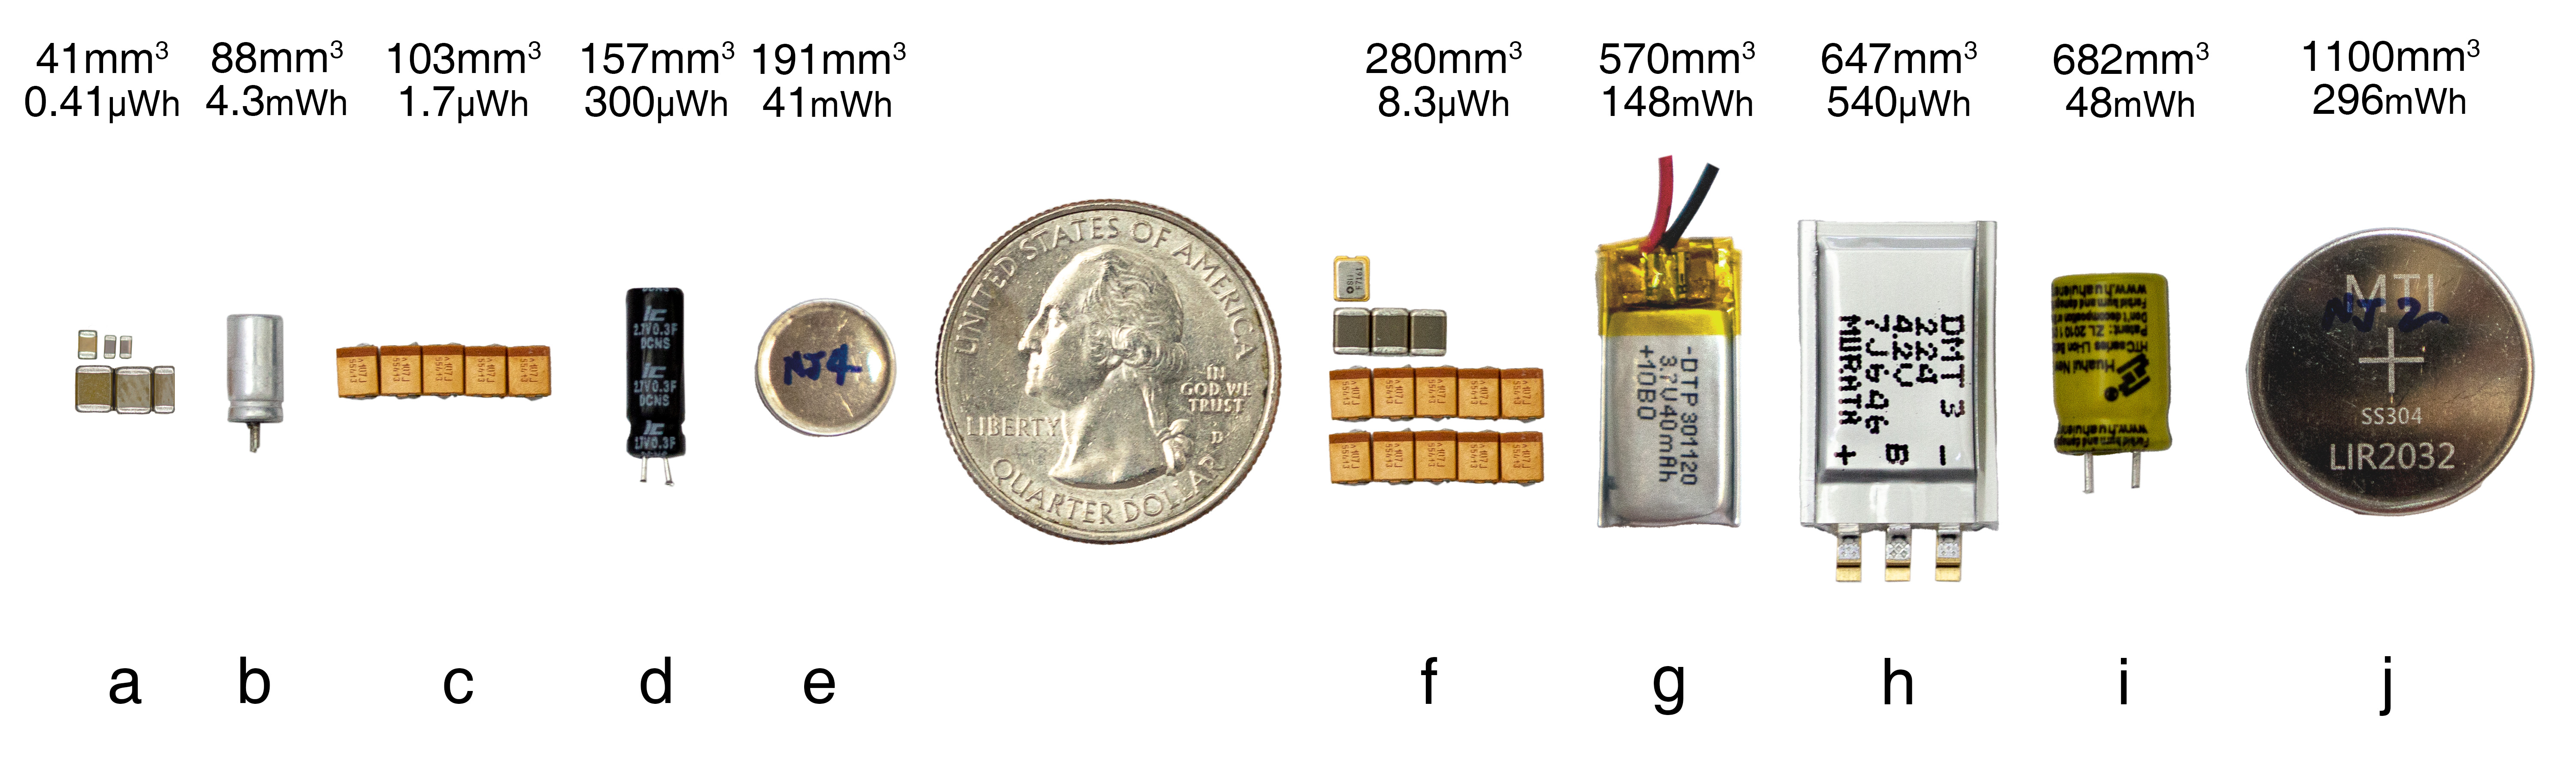
\includegraphics[width=\columnwidth]{figs/batteries/cap_lto_size_compare}
  \caption{
    A size comparison of energy storage methods including capacitors, supercapacitors, and batteries.
    \normalfont
    They are ordered left to right, by their
    (total) volume. Total volumes and energy storage are listed above the respective device.
    Configuration
    \textbf{(a)}, \textbf{(c)} and \textbf{(f)} represent the energy storage configurations used
    in the Flicker platfrom with BLE and several sensors~\cite{hesterFlicker17}, the Solar Monjolo~\cite{campbellEnergy14} and the Capybara temperature
    monitor and alarm~\cite{colinReconfigurable18}, which have total
    capacitances and energy capacities of 119\ssi{\micro\farad} (0.41\ssi{\micro\Wh} at 5~V), 500\ssi{\micro\farad} (1.7\ssi{\micro\Wh} at 5~V)
    and 8.8\ssi{\milli\farad} (8.3\ssi{\micro\Wh} at 2.6~V), respectively. Capacitors
    \textbf{(d)}~\cite{illinoisCap} and \textbf{(h)}~\cite{murataCap} are large
    supercapacitors available on the Capybara platform and have the
    capacitances and energy capacities of 300\ssi{\milli\farad} (300\ssi{\micro\Wh} at 2.7\ssi{\volt}) and 220\ssi{\milli\farad}
    (540\ssi{\micro\Wh} at 4.2\ssi{\volt}) respectively.  Devices \textbf{(b)} and \textbf{(i)} are 
    small LTO battery cells with 1.8\ssi{\milli\Ah} (4.3\ssi{\milli\Wh} at 2.4~V) and 20\ssi{\milli\Ah} (48\ssi{\milli\Wh}
    at 2.4\ssi{\volt}) capacity respectively~\cite{LTODatasheet2}. Devices \textbf{(e)} and \textbf{(j)} are small prototype Li-ion coin cells with 11\ssi{\milli\Ah} (41\ssi{\milli\Wh} at 3.7~V) and 80\ssi{\milli\Ah} (296\ssi{\milli\Wh} at 3.7~V) respectively~\cite{millibatNimbus}. Device \textbf{g} is a traditional Lithium Polymer pouch cell with 40\ssi{\milli\Ah} (148\ssi{\milli\Wh} at 3.7~V)~\cite{sparkfunPouch}.
    The LTO battery \textbf{(b)} and the Li-ion coin cell \textbf{(e)} are among the smallest of all configurations of energy storage
    presented here and also provide one to two orders of magnitude more energy capacity
    compared to \textbf{(f)}, the largest supercapacitor presented.
  }
\end{definefigure}

\begin{definefigure}{fig:battery:ragone}
\centering
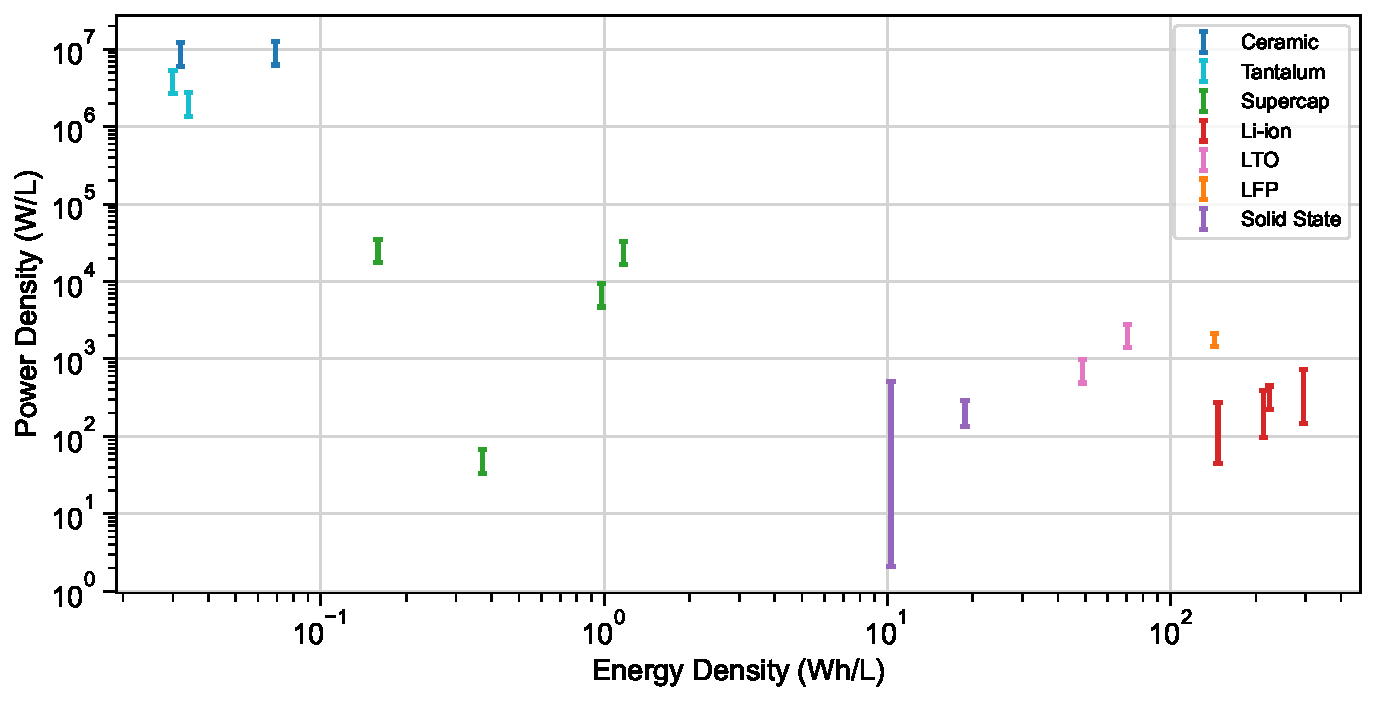
\includegraphics[width=\columnwidth]{figs/ragone}
\caption{Ragone plot for components listed in \cref{tab:battery:cost}, in log-log scale. A ragone plot directly compares power and energy density for different devices. Ceramic and tantalum capacitors are very power dense, but provide abysmal energy density. Batteries provide superior energy density, are less power dense. Supercapacitors exist between these two extremes. Even though batteries do not provide comparable power density to either capacitors or supercapacitors, they can still provide sufficient power for common wireless sensor workloads, like operating a short or long range radio.}
\end{definefigure}

\begin{definefigure}{fig:battery:eperd}
\centering
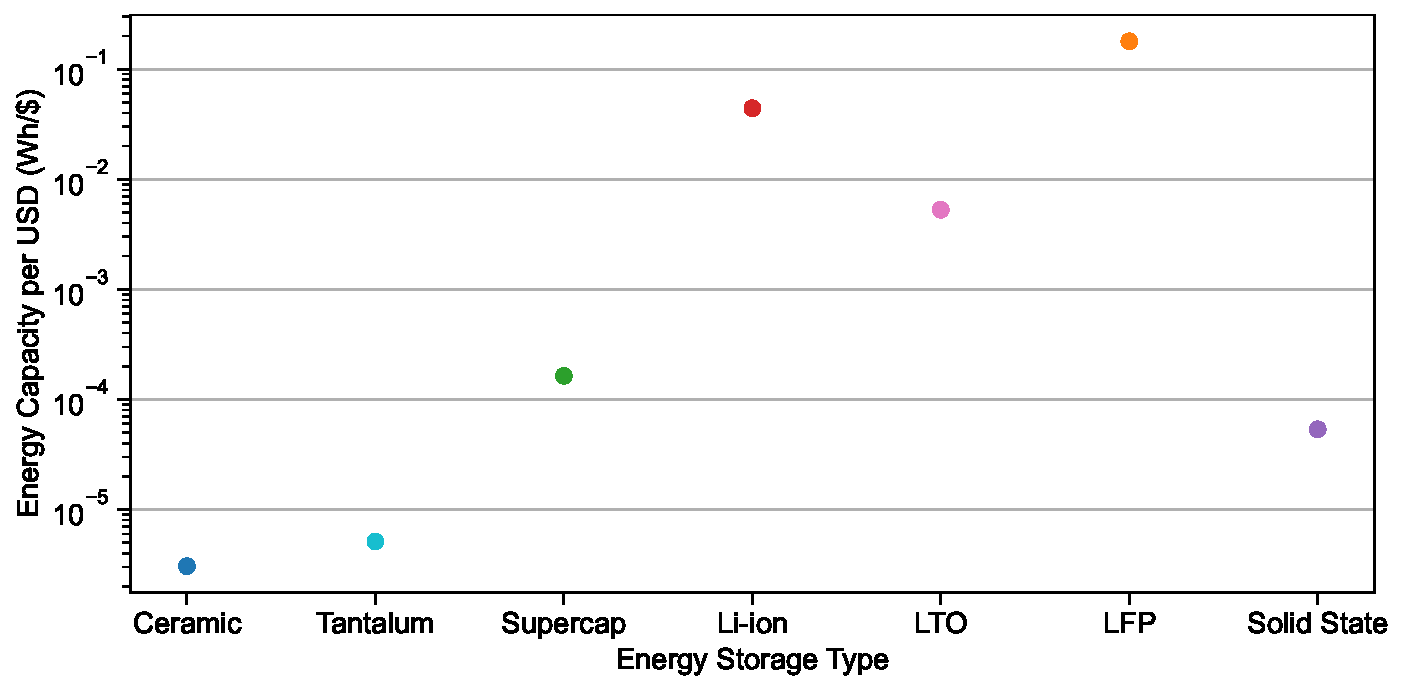
\includegraphics[width=\columnwidth]{figs/energy_per_cost.pdf}
\caption{
    Average energy capacity for various technologies selected in \cref{tab:battery:cost}, normalized by price in USD. Wherever possible, component costs were determined by their price in the United States. In regards to energy capacity, batteries offer 3-5 orders of magnitude more energy capacity per dollar than ceramic and tantalum capacitors. Batteries also offer 2-3 orders of magnitude more capacity than supercapacitors.
}
\end{definefigure}

\chapter{Utilizing Capacity for Untethered Image Sensing}
\label{cha:permacam}

\section{Evaluating an Existing System through Simulation}

\section{Capacity-focused Redesign of an Existing System}


\section{Summary}
\chapter{Utilizing Capacity for Capable Computation and Inference}
\label{cha:capability}

\section{Compute and Communication Energy Tradeoff}

\section{Increasing Compute Capability with an Accelerator}

\section{Summary}

\chapter{Conclusion}
\label{chap:conc}

\section{The Local Compute versus Transmit Trade-Off}

For Camaroptera, the decision to include local inference to filter out non-interesting images was worth it due to cost of transmitting images. This is not necessarily the case with Permacam, where the costs of doing the inference and transmitting images is about equal.
Embedded computing is improving in power efficiency at higher rate than active radios.


\subsection{Power Trends}

Figure: Energy per bit vs \ssi[per-mode=symbol]{\micro\ampere\per\mega\hertz} for radio/processor over time.

\subsection{Computing Trends}
Introduction and improvement of low power embedded accelerators for DSP and neural net inference. What are the trends? How to compare with conventional Cortex M cores and each other?

\subsection{The Constant Need for More Energy}
As computing efficiency increases, sensor data processing complexity will continue to increase, resulting in sensors that do more for the same amount of power. These sensors will require all the energy they can get. 

\section{What Primitives will Future Energy Harvesting Sensors Need?}

A wish list for future sensor design primitives.

\begin{enumerate}
    \item Coulomb counting for energy income and used energy
    \item Separate power domains for state preservation and active operation
    \item More memory and memory protection (virtual memory?) for more sophisticated programs and usability
    \item Parallel interfaces on low power SoCs
\end{enumerate}

\section{Conclusion}


% \appendix
% \chapter{More Monticello Candidates}

\printbibliography
\end{document}
